\documentclass[12pt]{ucsd}
% mathptmx is a Times Roman look-alike (don't use the times package)
% It isn't clear if Times is required. The OGS manual lists several
% "standard fonts" but never says they need to be used.
\usepackage{mathptmx}
\usepackage[NoDate]{currvita}
\usepackage{array}
\usepackage{tabularx}
\usepackage{booktabs}
\usepackage{subfig}
\usepackage{ragged2e}
\usepackage{microtype}
\usepackage[breaklinks=true,pdfborder={0 0 0}]{hyperref}
\usepackage{graphicx}
% ---
\usepackage{color}             % for color and textcolor
\usepackage{xspace}            % for heppennames
\usepackage{pifont}            % for dingbats
\usepackage[export]{adjustbox} % for valign in subfloats
% ---
\AtBeginDocument{%
	\settowidth\cvlabelwidth{\cvlabelfont 0000--0000}%
}
% ---
% Pennames (TDR aliases for particles)
\usepackage{sty/hepparticles}
\usepackage{sty/heppennames2}
% Custom aliases
\usepackage{sty/aliases}
% ---

% OGS recommends increasing the margins slightly.
\increasemargins{.1in}

% These are just for testing/examples, delete them
\usepackage{trace}
%\usepackage{showframe} % This package was just to see page margins
\usepackage[english]{babel}
\usepackage{blindtext}
\overfullrule5pt
% ---
% Reference for quotes
\def\signed #1{{\\ \hspace*{\fill}(#1)}}
% Custom quote environments
\newsavebox\mybox
\newenvironment{aquote}[1]
  {\savebox\mybox{#1}\begin{quote}\itshape}
  {\signed{\usebox\mybox}\end{quote}}
\newenvironment{epiquote}[1]
  {\savebox\mybox{#1}\noindent\ignorespaces\begin{flushright}\itshape}
  {\signed{\usebox\mybox}\vfil\end{flushright}}
% ---

% Required information
\title{Measurements of the Higgs Boson through Vector Boson Scattering and Software and Computing for Exascale Data Science}
\author{Jonathan Kasuke Guiang}
\degree{Physics}{Doctor of Philosophy}
% Each member of the committee should be listed as Professor Foo Bar.
% If Professor is not the correct title for one, then titles should be
% omitted entirely.
\chair{Professor Frank W\"urthwein}
% Your committee members (other than the chairs) must be in alphabetical order
\committee{Professor Sekhar Chivukula}
\committee{Professor Albert Hsiao}
\committee{Professor Arun Kumar}
\committee{Professor Michael Norman}
\committee{Professor Avraham Yagil}
\degreeyear{2024}

% Start the document
\begin{document}
% Begin with frontmatter and so forth
\frontmatter
\maketitle
\makecopyright
\makesignature

% --- Dedication ---
\begin{dedication}
\setsinglespacing
\parindent0pt\parskip\baselineskip
\begin{center}
This dissertation is dedicated to my wife Rosemary and the future we are building together; 
to my parents, Orlando and Cynthia Guiang, and my sister, Christina Guiang; 
to grandpa and grandma, John and Tsuneko Hashiguchi; 
to abuelo and abuela, Rufino and Aurelia Guiang; 
to the thousands of miles traveled, centuries of hardship endured, decades of triumph celebrated, and many wonderous years yet to come. 
I love you all more than words can express.
\end{center}
\end{dedication}


% --- Epigraph ---
\begin{epigraph}
\vskip0pt plus.5fil
\setsinglespacing

\begin{epiquote}{William Blake, Auguries of Innocence, 1863}
    To see a World in a Grain of Sand \\
    And a Heaven in a Wild Flower \\
    Hold Infinity in the palm of your hand \\
    And Eternity in an hour
\end{epiquote}

\begin{epiquote}{James Joyce, interview with Arthur Power, 1921}
    In the particular is contained the universal.
\end{epiquote}

\begin{epiquote}{James Baldwin, The Paris Review, 1984}
    Talent is insignificant. \\
    I know a lot of talented ruins. \\
    Beyond talent lie all \\
    the usual words: discipline, love, luck, \\ 
    but, most of all, endurance.
\end{epiquote}

\end{epigraph}


% --- Table of contents ---
% Next comes the table of contents, list of figures, list of tables,
% etc. If you have code listings, you can use \listoflistings (or
% \lstlistoflistings) to have it be produced here as well. Same with
% \listofalgorithms.
\tableofcontents
\listoffigures
\listoftables

% --- Acknowledgements ---
\begin{acknowledgements}
Recorded in this dissertation, in great detail, are my contributions to a grand scientific enterprise. 
What is not documented, however, are the struggles, doubts, heartache, frustrations, and so much more that lie beyond the histograms, tables, and physics prose. 
Through each of these challenges, I am fortunate to have been surrounded by incredible people who ran beside me in the best of times, and dragged me along in the worst. 
Please find below my best attempt at thanking them, in mere sentences, for making all of this---and all that is to come---possible. 

Foremost, I owe boundless thanks to my incredible family. 
First, to Mom and Dad, thank you for raising me in a home full of love and imagination and for all of your work and sacrifice upon which my life, career, and now this dissertation have been built upon. 
And to Christina, my big sister: thank you for your strength and courage, for all of our memories growing up together (except, perhaps, those that ended with my injury), and for inspiring me to be bold. 
I am also fortunate to have spent a great deal of time with my grandparents, John and Tsuneko Hashiguchi---thank you, grandma and grandpa, for teaching me to be good and honest and for showing me how to persevere. 
Amidst all of my ``found'' family---family by bond, not blood---I must, most of all, thank my uncle, John Sanders: thank you for putting up with your briny nickname, for every phone call, for your humor (even when it is at my expense), and for helping me at every stage of my career. 
Finally, to my wife Rosemary, who has brightened my life in every way: thank you for your kindness and compassion, for everything that you are, I love you more than anything. 
I hope that today and on every day after, I can make you all proud.

I am equally grateful for the many mentors I have had in my relatively short academic career, organized here by the institution at which we met. 
Starting with UCSD, I thank Prof. Frank W\"urthwein, my advisor, who believed in me, guided me through all of my achievements, and flew me around the world---thank you, Frank, for everything. 
And to Prof. Avi Yagil, who served as my co-advisor: thank you for challenging, uplifting, and educating me. 
I also owe many thanks to Prof. Philip Chang who, in many ways, was also my co-advisor. 
For hours of conversation via Zoom and over 130\,000 Skype messages, for even more hours of physics and C++ lessons, and for your nearly endless patience: thank you, Philip. 
Next, from my alma mater, UCSB, I am ever indebted to Prof. Claudio Campagnari for taking me in and completely altering the course of my life. 
Claudio gave me purpose during what was, probably unbeknownst to him, a very difficult time for me personally---thank you, Claudio; without you, this dissertation simply would not exist. 
Also, Claudio's former students and postdocs were my first and most formative mentors. 
Thanks, in particular, to Dr. Nick Amin for teaching me everything I know. 
Thanks also Dr. Bennett Marsh, who mentored me across multiple projects---I am a better leader, person, and scientist thanks to Nick and Bennett. 
And to Prof. Indara Suarez, who welcomed me into particle physics and pushed me to meet my true potential: thank you for the high-octane tour of Boston in your Mustang, your thoughtful mentorship, and your constant support. 

I must also thank all of the members, past and present, of the illustrious ``Surf n' Turf'' (SNT) empire, whose dominion stretches far across the western world. 
It has been a privilege to serve as your Data Librarian, and I am deeply grateful to each of you, though, unfortunately, I do not have space to list all of you. 
Therefore, my thanks are extended, but not limited to the following SNT'ers: Prof. Frank Golf, Dr. Daniel Spitzbart, Dr. Sam May, Aashay Arora, Dr. Slava Krutelyov, and former SNT'er Jerry Ling.

In addition to all of the aforementioned physicists, I have had the privilege of working alongside a number of incredible engineers whom I would like to mention here. 
In particular, I would like to thank Diego D\'{a}vila for patiently teaching some computer science to a budding physicist and for being a great mentor and friend. 
Thanks also to Terrence Martin for keeping our equipment running, teaching me how to deadlift, and for your amazing board game parties! 

With the due date of this dissertation rapidly approaching, I would like to end this section by acknowledging some of my incredible friends. 
To Joey Incandela, my physics brother (and best man): thank you for the many nights of gaming (despite the 3-hour time difference), for keeping me sane, and for your compassion and spirit. 
To Gabe Hernandez, my ex-physics brother (and ex-roommate): thank you for the silly inside jokes, for your constant guidance and encouragement, and for accompanying me to the base of Mt. San Jacinto, where I finished writing this dissertation amidst pizza, cookies, and the pines. 
To Grady Kestler, last but not least, my partner in crime: thank you for Sunday Night Games, for getting me through Stat. Mech., and for your camaraderie and insight. 
And to everyone else who has helped me along my journey: please know that I am sincerely thankful, and that I will endeavor to honor all of you with what I can contribute to the world. 

Through the Sloan Scholar program at UCSD, the Alfred P. Sloan Foundation provided financial and moral support for the work presented in this dissertation. 
To Shana Slebioda, Sinai Cota, and the Sloan Foundation: thank you!

Chapter~\ref{ch:lhc_cms} describes the Large Hadron Collider (LHC) and the CMS Experiment. 
The figures used in this chapter are materials produced by or for CERN and were released by CERN for informational use under CERN copyright. 
The description of the LHC and CMS are derived from publicly available material and the relevant technical design reports. 

Chapter~\ref{ch:vbswh} describes a search for the production of a W and Higgs boson via vector boson scattering, using data recorded by the CMS experiment from 2016 to 2018. 
It is a partial reproduction of the paper ``Study of WH production through vector boson scattering and extraction of the relative sign of the W and Z couplings to the Higgs boson in proton-proton collisions at $\sqrt{s} = 13\TeV$,'' submitted to PLB (arXiv:2405.16566). 
My individual contribution to this work was significant. 
I participated in its ideation by working with Prof. Philip Chang (in secret, at first) to make the initial calculations of the feasibility of the measurement. 
Then, I personally implemented the entire analysis, from basic selections, to the optimization of the signal region, to the background estimation and evaluation of systematic uncertainties.

Chapter~\ref{ch:vbsvvh} describes a search for the production of a Higgs boson and two vector bosons via vector boson scattering, using data recorded by the CMS experiment from 2016 to 2018. 
It is a partial reproduction of a paper being prepared for submission for publication. 
I worked as part of a multi-institutional team that, together, implemented the three main channels of this analysis. 
However, I personally drove the channel that I worked on. 
On top of implementing the analysis itself (from selections to systematic uncertainties), I also implemented the training pipeline for the deep neural network used for the final result in both my work and the other most sensitive channel of the combined analysis.

Chapter~\ref{ch:lst} describes improvements to the Line Segment Tracking algorithm using machine learning. 
It is a partial reproduction of the paper ``Improving tracking algorithms with machine learning: a case for line-segment tracking at the High Luminosity LHC,'' in the proceedings of Connecting the Dots 2023 (arXiv:2403.13166). 
This work is part of a larger effort to produce a highly parallelizable line-segment based tracking (LST) algorithm. 
My personal contribution included the development and training of a machine learning algorithm towards improving track-finding performance, and the eventual integration of it into the LST algorithm.

Chapter~\ref{ch:cyber} describes the development of software-defined networking (SDN) capabilities within the LHC data distribution cyberinfrastructure. 
It is a partial reproduction of the paper ``Managed Network Services for Exascale Data Movement Across Large Global Scientific Collaborations,'' in the proceedings of XLOOP 2022 (doi:10.1109/XLOOP56614.2022.00008). 
I personally developed the first version of the software that implements the interoperation of SDN into the LHC data management software, with guidance from research engineers at the SDSC and ESNet. 
I also configured the testbed of this system and orchestrated some of the first proof-of-concept tests. 
Diego D\'{a}vila, Aashay Arora, Tom Lehman, and Xi Yang were all instrumental in the success and continued progress of this work.

\end{acknowledgements}


% --- Vita ---
% Stupid vita goes next
\begin{vita}
\noindent
\begin{cv}{}
\begin{cvlist}{}
\item[2019] Bachelor of Science, University of California, Santa Barbara
\item[2019--2020] Teaching Assistant, University of California, San Diego
\item[2020--2024] Research Assistant, University of California, San Diego
\item[2023] Master of Science, University of California, San Diego
\item[2024] Doctor of Philosophy, University of California, San Diego
\end{cvlist}
\end{cv}

% This puts in the PUBLICATIONS header. Note that it appears inside
% the vita environment. It is optional.
\publications
\noindent Guiang, J. et al. (2023). 
\textit{Improving tracking algorithms with machine learning: a case for line-segment tracking at the High Luminosity LHC}
In 8th International Connecting The Dots Workshop. arXiv:2207.08207.
\newline
\newline
\noindent Aashay Arora, Jonathan Guiang, Diego Davila, Frank Würthwein, Justas Balcas, \& Harvey Newman (2023). 
\textit{400Gbps benchmark of XRootD HTTP-TPC.}
In 26th International Conference on Computing in High Energy \& Nuclear Physics. arXiv:2312.1258.
\newline
\newline
\noindent W\"urthwein, F., Guiang, J. et al. (2022). 
\textit{Managed Network Services for Exascale Data Movement Across Large Global Scientific Collaborations.}
In 2022 4th Annual Workshop on Extreme-scale Experiment-in-the-Loop Computing (pp. 16-19). IEEE Computer Society.
\newline
\newline
\noindent Guiang, J. et al. (2022). 
\textit{Integrating End-to-End Exascale SDN into the LHC Data Distribution Cyberinfrastructure.}
In Practice and Experience in Advanced Research Computing. Association for Computing Machinery.
\newline
\newline
\noindent Fajardo, E., ..., Guiang, J. et al. (2020). 
\textit{Moving the California distributed CMS XCache from bare metal into containers using Kubernetes.}
In 24th International Conference on Computing in High Energy \& Nuclear Physics. EPJ Web of Conferences.
\newline
\newline
\noindent Ball, A., ..., Guiang, J. et al. (2020). 
\textit{Search for millicharged particles in proton-proton collisions at $\sqrt{s} = 13\TeV$.}
Physical Review D, 102(3).
\end{vita}


% --- Abstract ---
% Put your maximum 350 word abstract here.
\begin{dissertationabstract}
    This dissertation presents the analyses of WH and VVH production through vector boson scattering (VBS). 
    The VBS WH analysis excludes scenarios where the HWW and HZZ couplings have opposite signs beyond 5 standard deviations. 
    The VBS VVH analysis places limits on the HHVV coupling between -0.03 and 2.04 times the Standard Model value. 
    Both analyses are based on proton-proton collision data recorded by the CMS experiment at the CERN LHC from 2016 to 2018 at a center-of-mass energy of 13 TeV, corresponding to an integrated luminosity of 138 fb$^{-1}$. 
    In addition, two projects for the high luminosity LHC upgrade are described: a highly parallelizable track-finding algorithm and managed networking for exabyte-scale data science. 
\end{dissertationabstract}


% --- Chapters ---
\mainmatter
\begin{dissertationintroduction}
\begin{aquote}{Carl Sagan, Cosmos: A Personal Voyage, 1980}
    We are a way for the cosmos to know itself.
\end{aquote}

\section*{Infinity in the palm of your hand}
This dissertation is based entirely on a simple question: what is everything made of? 
For the vast majority of human history, all answers to this question were equally immaterial, yet for millennia, people with enough time on their hands and food in their bellies have wondered about it---from the Greek philosopher Democritus~\cite{Taylor1419554}, to the Hindu scholar Kan\=ada (or, ``atom-eater''), and probably long before them. 
Over time, philosophical musing transformed into scientific inquiry as we linked the question of \textit{what} to \textit{how} and \textit{why}. 
How does water turn to ice? 
Why are metals different? 
How does charcoal and iron form steel? 
Why does the sun shine? 
How did everything come to be? 
And as science progressed, faltered, corrected, and progressed again (and again, and again), patterns began to emerge around these questions, presented here as what David Griffiths calls a ``folk history'' for brevity, with inspiration taken heavily from the first chapter of his revered textbook~\cite{GriffithsParticle}.  

In 1808, the chemist John Dalton published the first\footnotemark{} atomic theory~\cite{Dalton1805, Dalton1808}, but the existence of the atom itself could not be directly verified. 
\footnotetext{
    Dalton's now legendary claim to this was hotly contested by his contemporary, William Higgins, although without much credence~\cite{HigginsClaim}.
}
However, nearly a century later, physicists including Henri Becquerel, Marie Curie, and J.J. Thompson found that certain elements and electronic apparatuses emitted different kinds of invisible radiation~\cite{Becquerel, Curie, RADVANYI2017544, Thompson}. 
In the decades following, they further realized that this radiation consisted of tiny particles\footnotemark{}, and Ernest Rutherford directed rays of these particles at thin sheets of metals, probing the subatomic scale for the first time. 
Based on these seminal experiments, Rutherford made a groundbreaking observation and two key deductions: % citations needed for Rutherford
\footnotetext{
    Namely photons (X-rays or $\gamma$ rays), electrons ($\beta$ rays), and helium ions (He$^{2+}$ or $\alpha$ rays). 
}
\begin{enumerate}
    \item \textit{Observation}: The atom exists\footnotemark{} and has a very small ``nucleus'' of positive charge.
    \item \textit{Deduction}: The nucleus is made of positively charged ``protons.''
    \item \textit{Deduction}: The nucleus is also made of ``neutrons'' which help keep it together.
\end{enumerate}
\footnotetext{
    It should be noted that Jean Perrin separately confirmed the existence of molecules, and thus reality of atoms, by proving experimentally that the random walk of a microscopic object suspended in liquid could only be due to collisions with the molecules of that liquid~\cite{Perrin}---a phenomenon first observed by the great botanist Robert Brown~\cite{Brown} (i.e. Brownian motion) and rigorously explained by Albert Einstein in one of his first papers~\cite{EinsteinBrownian}.
}
Through their work in the lab, Rutherford, Curie, and the other atomic pioneers had unknowingly stumbled upon the surface of an even greater truth than Democritus, Kan\=ada, or anyone else could have imagined. 

Albert Einstein, Max Planck, Niels Bohr, and others had begun writing down corrections to ``classical'' physics at the turn of the 19\ts{th} century in order to better describe unexplained phenomena observed in the lab~\cite{EinsteinPhotoelectric, Planck, Bohr}. 
By the time Rutherford's neutrons had been discovered by James Chadwick in 1932~\cite{Chadwick1932}, a cadre of theorists, including many of the most well-known physicists in history\footnotemark{}, had formed around Quantum Mechanics.
This ``new physics'' extended the early results of Einstein, Planck, and Bohr into a more complete theory describing the subatomic world, then thought to only include protons, neutrons, and electrons. 
\footnotetext{Werner Heisenberg, Erwin Schr\"odinger, and Robert Oppenheimer to name a few.}
Over the next decades, a slew of new particles were discovered: 
anti-matter was produced in the lab; % citation needed
electrons were joined by muons and neutrinos in the ``lepton'' family; % citations needed
an enormous crowd of more massive particles (baryons and mesons which together comprise the families of hadrons) akin to protons and neutrons were observed. % select citations needed
While some of these particles were already thought to exist, experimental results had, momentarily, outpaced theory. 
Theorists were developing new ideas on how to classify or relate different particles, but the ever-growing ``particle zoo'' was otherwise in disarray. 
However, as is a consistent pattern in history, science progressed, faltered, corrected, and progressed again (and again, and again), and patterns began to emerge. 

\section*{A glorious victory parade}
It began with Murray Gell-Mann, who, among others, saw a pattern in the deluge of new particles being discovered. 
He arranged the numerous hadrons in geometric patterns---octagons, triangles, and so forth---according to their properties~\cite{Gell-Mann:1961omu}, and found that his unusual diagrams held predictive power: some of his shapes were missing vertices, which were later found to be particles exactly matching the expectations from Gell-Mann's theory~\cite{PhysRevLett.12.204}. 
With confidence in Gell-Mann's so-called ``Eightfold Way'' established, a natural question arose: what is the significance of these patterns? 
Gell-Mann himself, and, separately, George Zweig, arrived at the answer: hadrons are not themselves fundamental particles; instead, they are composed of truly fundamental particles called ``quarks''~\cite{Lichtenberg:784713}, and the Eightfold Way diagrams corresponded to different configurations of quarks and the properties of those configurations.
Similar to Rutherford's experiments 50 years prior, wherein beams of particles were used to probe the structure of the atom, the reality of quarks could be probed by firing beams of electrons at protons, revealing their inner structure~\cite{PhysRevLett.23.930, PhysRevLett.23.935}. 
Though these experiments showed only that the proton had three constituent ``partons,'' they provided initial evidence for the existence of quarks.
And so the field progressed, with families of particles filling out into neat organizations: 
the quarks became a family of six, divided into three generations (up/down, charm/strange, top/bottom); % select citations needed
the leptons, with the addition of the tau and its neutrino, satisfyingly also totaled six particles divided into three generations ($\Pe/\PGne$, $\PGm/\PGnGm$, $\PGt/\PGnGt$); % citation for tau needed
the photon was joined by the gluon, \PW, \PZ, and Higgs boson~\cite{ATLASdisc, CMSdisc}, forming the family of bosons. % select citations needed
At the same time, a beautiful, yet deeply perplexing, quantum field theory was developing, which describes the interactions between these particles. 
In the words of the great Sydney Coleman~\cite{Coleman}:
\begin{quote}
    This was a great time [1966 to 1979] to be a high-energy theorist, the period of the famous triumph of quantum field theory. 
    And what a triumph it was, in the old sense of the word: a glorious victory parade, full of wonderful things brought back from far places to make the spectator gasp with awe and laugh with joy. 
\end{quote}
So began the Standard Model of particle physics: with groundbreaking discoveries and a scientific ``victory parade,'' which together still represent the largest fraction of Nobel Prizes by field~\cite{ParticleNobels}. 

\section*{There and back again}
The Standard Model has, despite remaining largely unchanged since the 1980s, withstood a tremendous amount of scrutiny across decades of intense study and many billions of dollars of scientific instrumentation. % citation or LHC xsec plot
It supplies, in principle, the answers to those questions posed at the beginning of this chapter: the sun's light, all of matter, and the origins of the universe itself are explained by the existence of, and interactions between, fundamental particles, which, in turn, form atoms, which form the structure of the material world. 
However, we quickly found that this theory of everything is really only a theory of some things, and long-known errors and inconsistencies---reserved for discussion in the next chapter---have been, much to the community's dismay, just as durable as the Standard Model has been otherwise. 
Particle physics has therefore reached a familiar inflection point, where we are left in anticipation of the next measurement that confirms an unusual approach or the next surprising discovery that leads the theory in an entirely new direction. 
Described in this document are the efforts of one graduate student, along with the invaluable support of his many colleagues, to contribute to this extraordinary enterprise. 
Together, we shall recount his journey, taking the perspective of the ``experimentalist.'' 
That is, very few formulas, axioms, and derivations---the language of theorists---are to be found in this dissertation. 
Instead, we will find tables of measurements, histograms, and some statistics. 
We will take general direction from the theory, then construct experiments to realize it in nature. 

This work is based on the proton-proton collision data collected by the Compact Muon Solenoid (CMS), a multi-billion dollar particle detector situated on the beamline of the Large Hadron Collider (LHC)---the most powerful particle collider and the single largest scientific instrument ever built, at the time of writing. 
At the risk of losing the reader who is not committed to reading the many pages that lie beyond this introduction, no new physics is documented here.
Instead, this humble submission, amongst over one thousand publications from the CMS Collaboration alone, represents a small contribution to the rich history documented above, demonstrating the continued success of a theory that dares to describe the entire universe.
\end{dissertationintroduction}

\chapter{A Beautiful Theory}
\begin{aquote}{Murray Gell-Mann, Beauty and truth in physics, 2007}
    What is especially striking and remarkable is that in fundamental physics 
    a beautiful or elegant theory is more likely to be right 
    than a theory that is inelegant.
\end{aquote}

\section{The Standard Model}
Put simply, the Standard Model (Fig.~\ref{fig:standard_model}) attempts to describe, at the most fundamental level, what the universe is made of and how it operates. 
So far, the content of the model is as follows: the universe is made of fermions (quarks and leptons), and it operates through the exchange of bosons (photons, gluons, W, Z, and H). 
That is, matter\footnotemark{} is composed of assemblies of fermions, which are held together, pushed apart, and otherwise interact via the fundamental forces ``transmitted'' by bosons. 
\footnotetext{With the notable exception of ``dark'' matter, which is discussed later in this chapter.}
The first and most familiar of these is the electromagnetic (EM) force because its carrier, the photon, is absorbed by the retinas in our eyes, enabling the fortunate majority of us with the gift of sight. 
Then, there is the weak force, carried by the W and Z bosons, which is responsible for the radioactive decay of certain elements. 
These first two forces are, today, understood to be unified into the ``electroweak'' (EW) force. 
Finally, there is the strong force, which holds the nuclei of atoms together. 
Alongside the forces, there is the Higgs mechanism, carried by the Higgs boson, which is responsible for giving the fundamental particles mass. 
Together, these forces and the Higgs mechanism---and gravity, whose omission here is left as a topic for another time---describe how \textit{everything} came to be and continues to be: from the sight of the sun in the sky, to the fusion reaction causing the sun to shine, to the formation of the sun and all of the other stars in the universe, to the first instance of creation itself. 
The entire universe is, we believe, the emergent motion from an elegant, infinite dance of fundamental particles. 

Of course, a stack of textbooks underlie the text above.
The concepts of fermions and bosons carry deeply insightful mathematical meaning derived originally in statistical mechanics, which was developed to describe the behavior of large ensembles of microscopic objects (like gases). 
Moreover, the particle ``zoo'' has been herded into the confines of the mathematical framework called quantum field theory (QFT), wherein particles are described as excitations of quantum ``fields'' and physical laws are realized as mathematical symmetries. 
Unfortunately, four to five years of attentive instruction and rigorous study across multiple subjects---including quantum mechanics, statistical mechanics, special relativity, and a bevy of mathematical formalism---are required to even begin reading QFT textbooks, and well over a lifetime may be required to fully understand them\footnotemark{}. 
\footnotetext{Even still, paraphrasing the great Prof. Aneesh Manohar, ``all QFT textbooks are wrong.''}
The Standard Model will instead, as promised, be described here from the perspective of an experimentalist: through hastily scrawled cartoons, rough calculations, and a great deal of hand-waving that, together, at least communicate the essential features of the theory. 

\begin{figure}[htb]
    \centering
    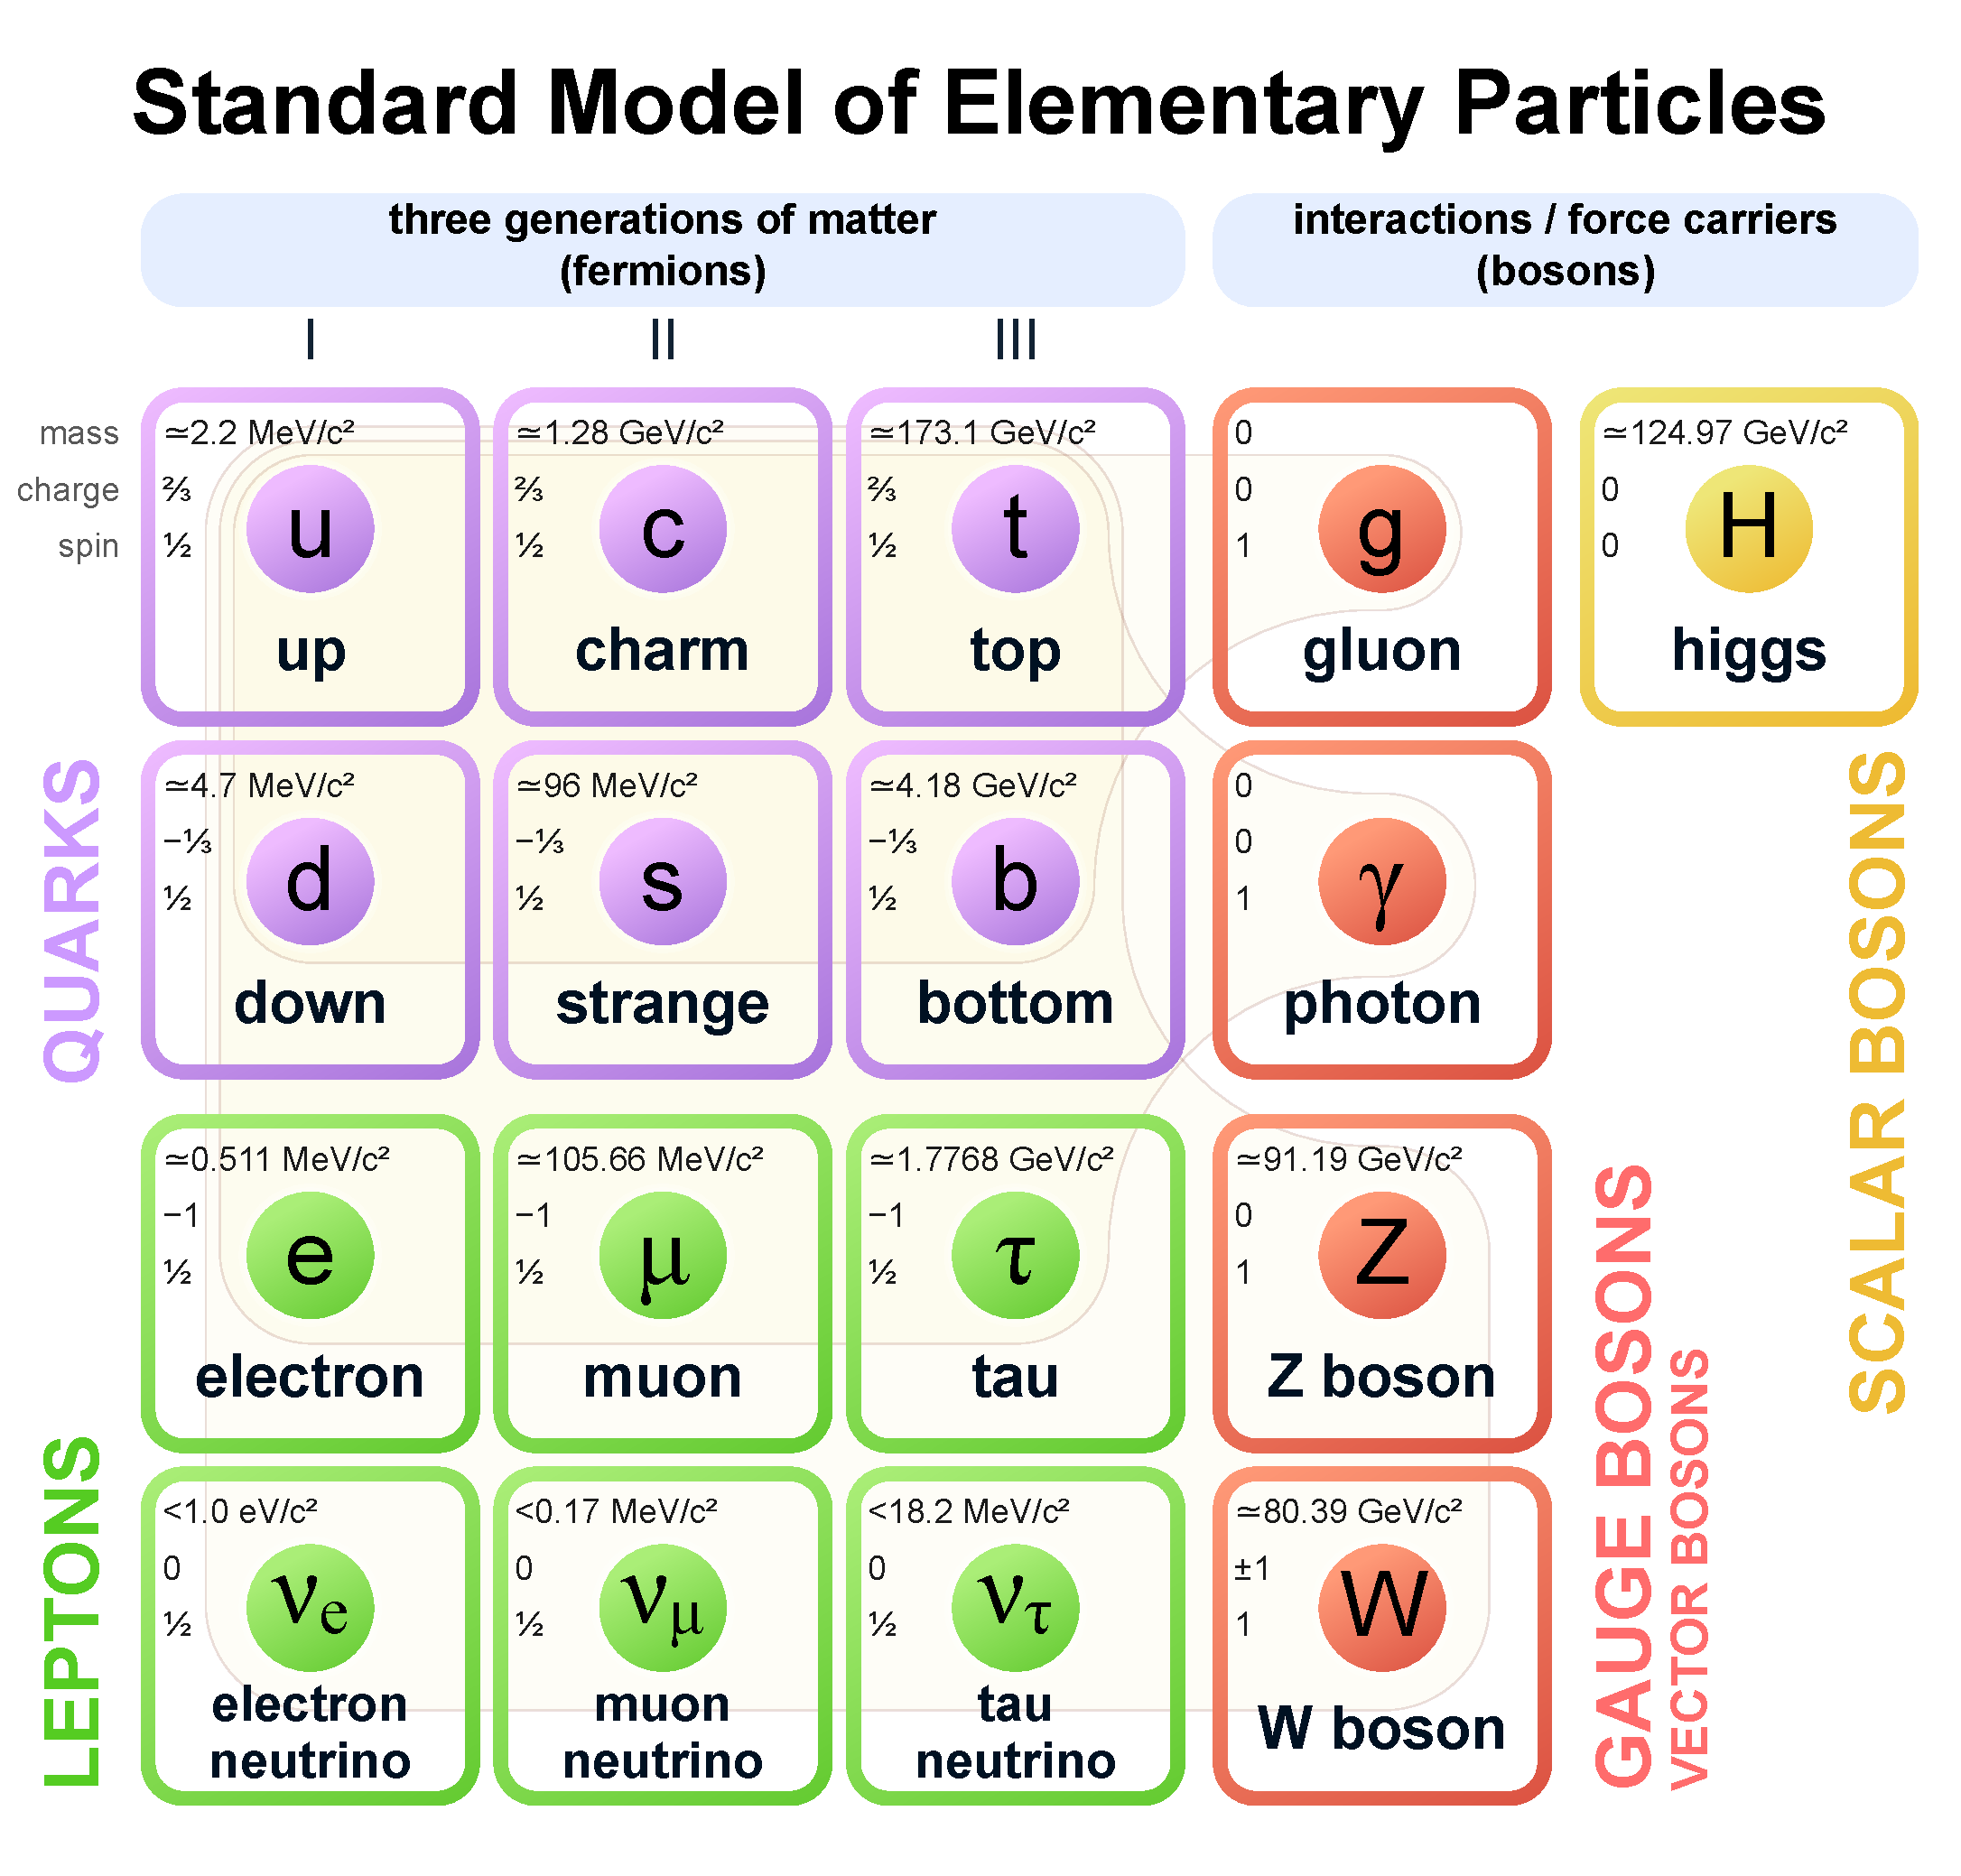
\includegraphics[width=0.9\textwidth]{fig/standard_model.pdf}
    \caption{
        The Standard Model.
    }
    \label{fig:standard_model}
\end{figure}

\subsection{Feynman diagrams}
Fortunately, there is way to encode essential Standard Model calculations in a simple drawing, so-called ``Feynman diagrams,'' which, consequently, help experimentalists keep track of physically allowed processes. 
In these pictures, time flows from left to right, while space is abstractly represented on the vertical axis\footnotemark{}. 
\footnotetext{In some dark corners of the physics community, these axes are switched, but this dissertation will not deviate from the configuration described here.}
The fundamental particles are represented by lines, and the intersections of three or four of these lines (Fig.~\ref{fig:sm_vertices}) represent interactions between the corresponding particles, so at least one of them must be a boson. 
For example, an electron emitting a photon (Fig.~\ref{fig:qed1}) is represented by an electron coming in from the left, the turning into a photon and an electron leaving the picture to the right. 
This same vertex can be rotated clockwise, such that it instead depicts the annihilation of an electron and positron into a photon (Fig.~\ref{fig:ee_to_g})---one of the electrons had to be replaced with its anti-particle (a positron) to conserve charge. 
Rotating it again, we see that it now represents an electron absorbing a photon (Fig.~\ref{fig:eg_to_e}). 
These vertices act as building blocks that can be rotated and fit together according to a set of rules that correspond to real physical laws. 
Thus, any fundamental physical process (e.g. Fig.~\ref{fig:beta_decay}) can be represented with a Feynman diagram. 
Feynman diagrams are not only a visual aid for remembering which processes are allowed, however, for they also encode precise calculations about that process which can, importantly, be verified by experiment.

\begin{figure}[htb]
    \centering
    \subfloat[]{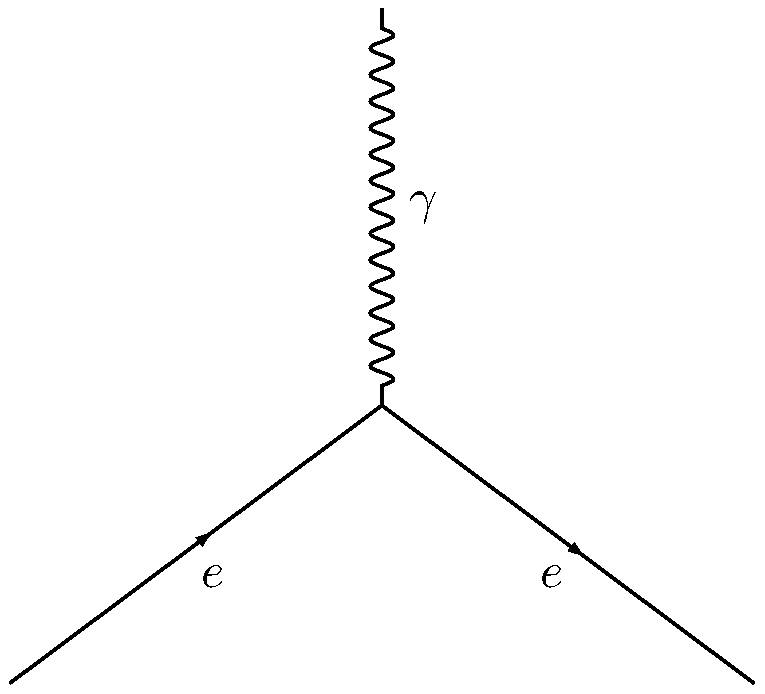
\includegraphics[width=0.25\textwidth]{fig/feynman/forces/qed_vertex.pdf}\label{fig:qed1}}\quad
    \subfloat[]{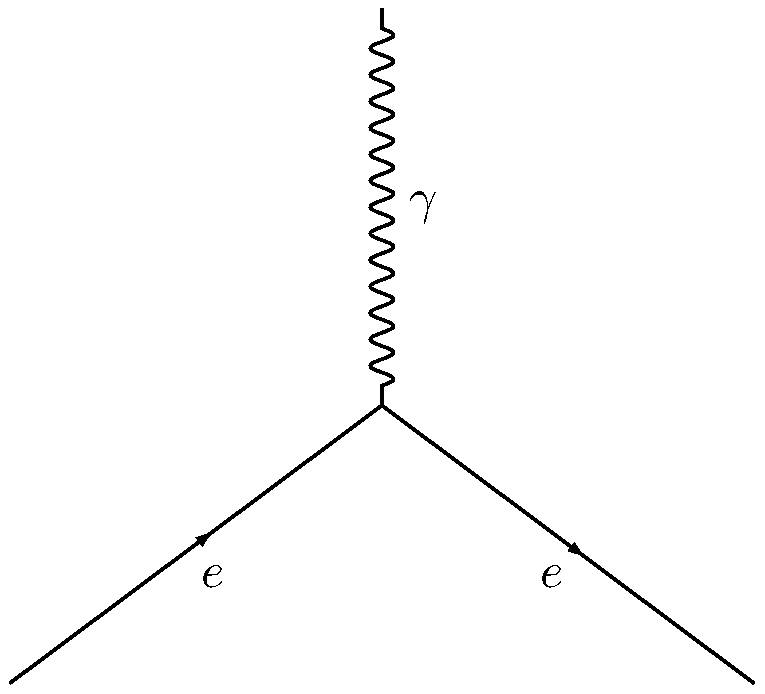
\includegraphics[width=0.25\textwidth]{fig/feynman/forces/qed_vertex.pdf}\label{fig:ewk1}}\quad
    \subfloat[]{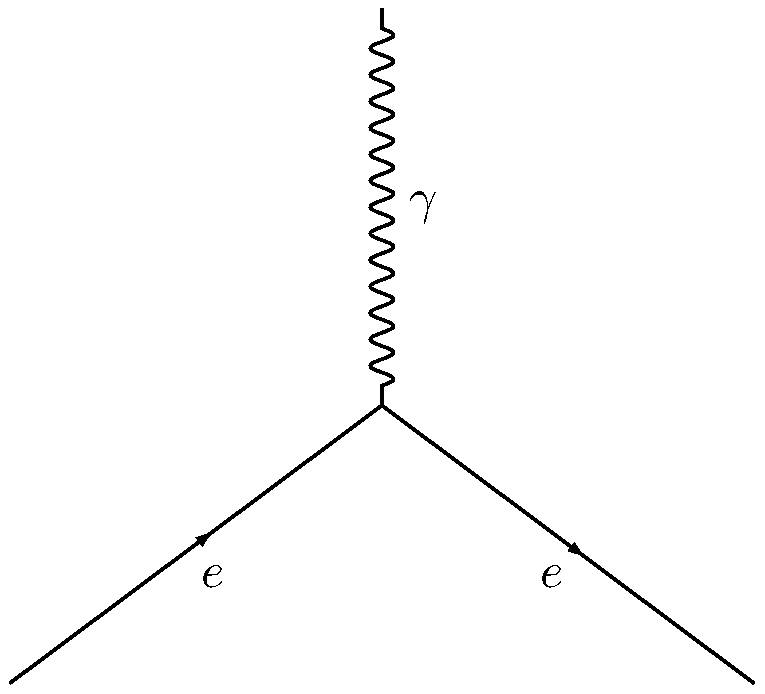
\includegraphics[width=0.25\textwidth]{fig/feynman/forces/qed_vertex.pdf}\label{fig:ewk2}}\\
    \subfloat[]{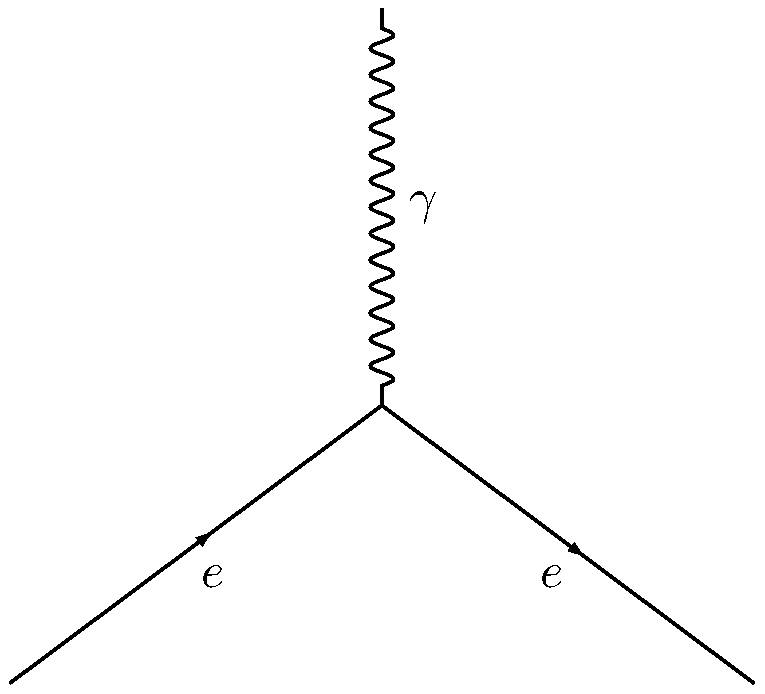
\includegraphics[width=0.25\textwidth]{fig/feynman/forces/qed_vertex.pdf}\label{fig:weak}}\quad
    \subfloat[]{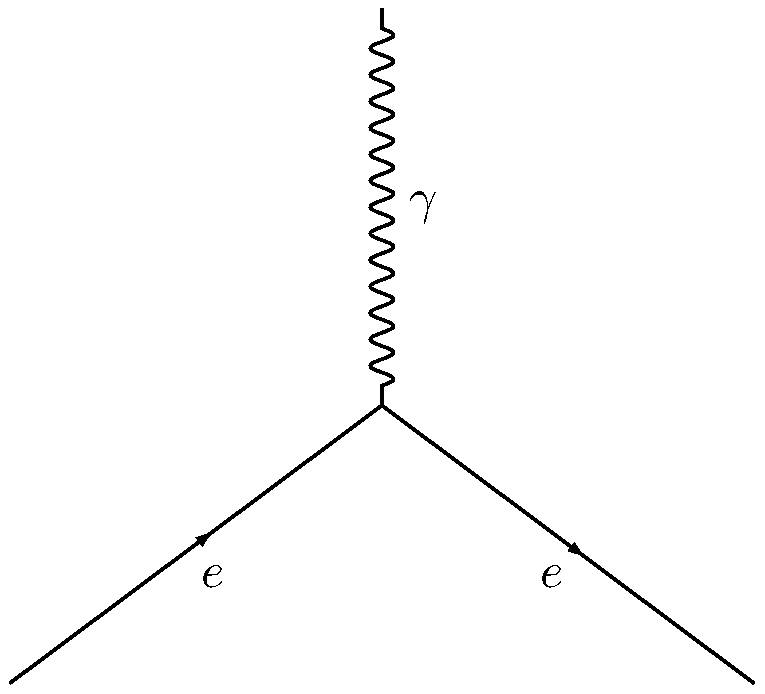
\includegraphics[width=0.25\textwidth]{fig/feynman/forces/qed_vertex.pdf}\label{fig:qcd1}}\quad
    \subfloat[]{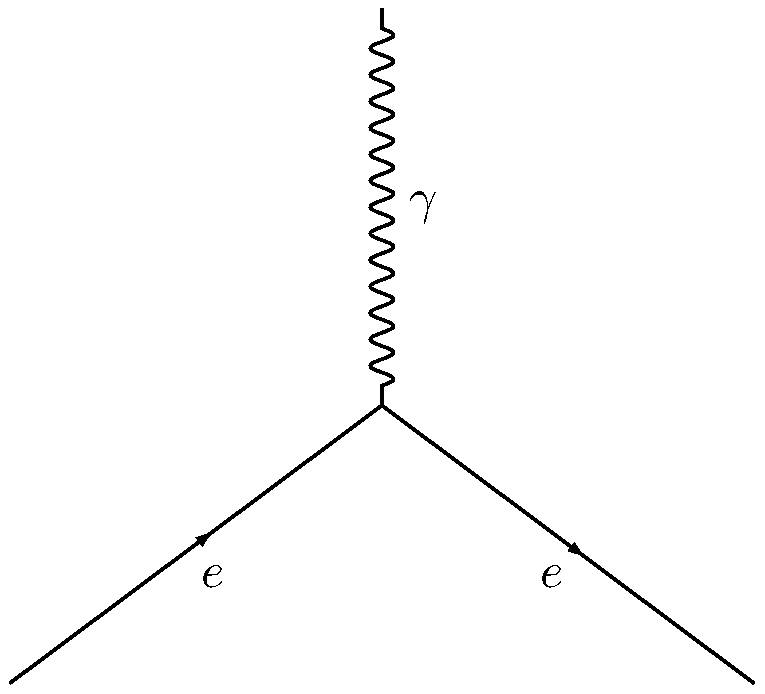
\includegraphics[width=0.25\textwidth]{fig/feynman/forces/qed_vertex.pdf}\label{fig:qcd2}}\\
    \subfloat[]{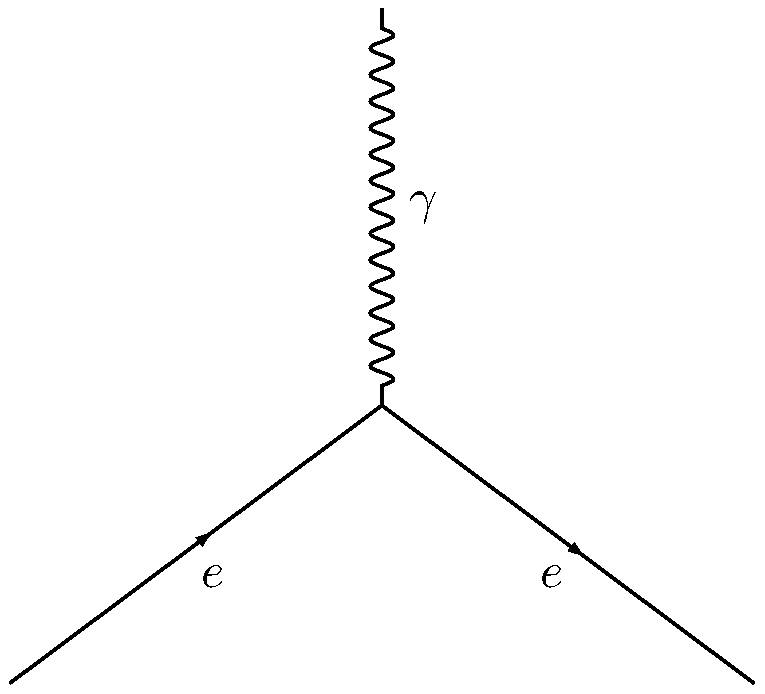
\includegraphics[width=0.25\textwidth]{fig/feynman/forces/qed_vertex.pdf}\label{fig:qcd3}}\quad
    \subfloat[]{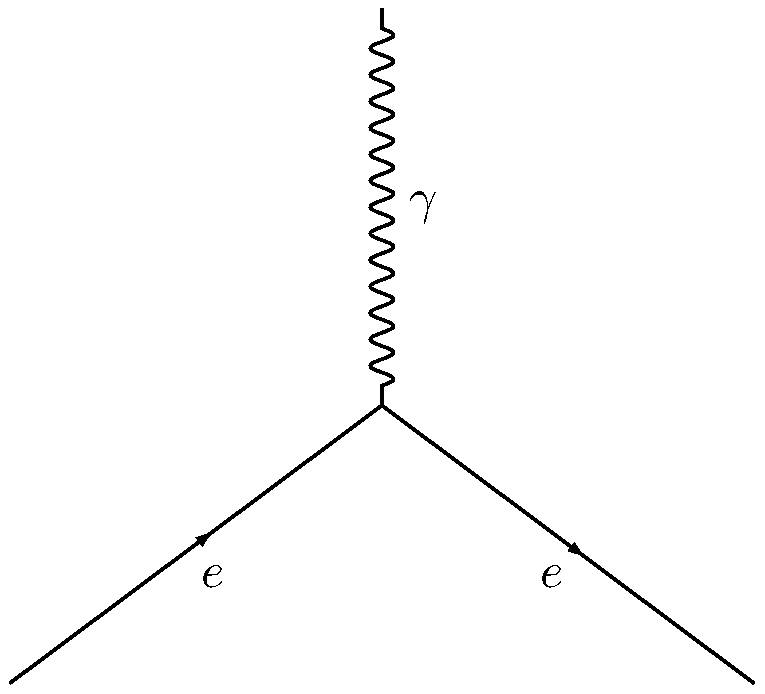
\includegraphics[width=0.25\textwidth]{fig/feynman/forces/qed_vertex.pdf}\label{fig:hig1}}\quad
    \subfloat[]{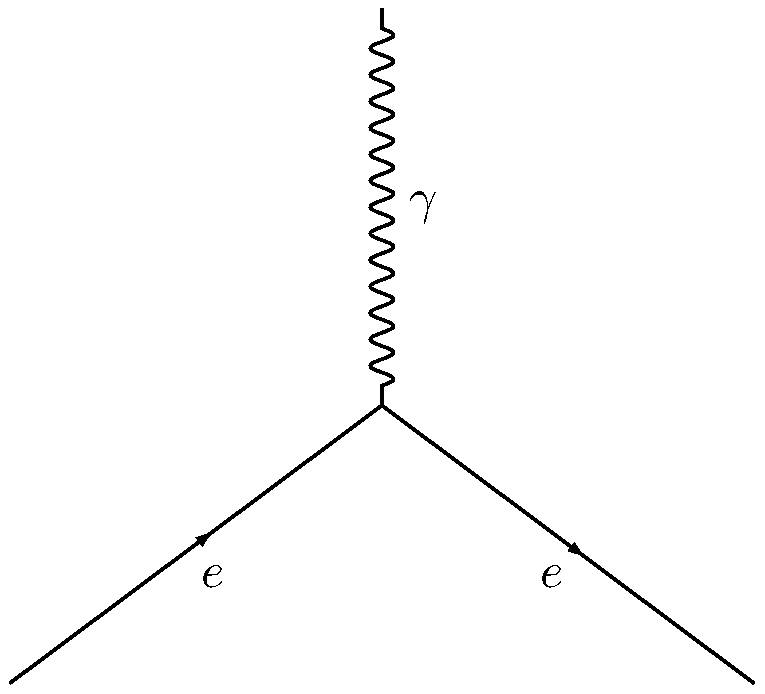
\includegraphics[width=0.25\textwidth]{fig/feynman/forces/qed_vertex.pdf}\label{fig:hig2}}
    \caption{
        The fundamental vertices in the Standard Model. 
        From left to right, top to bottom: 
        (a) electromagnetic; (b), (c) electroweak; (d) weak; (e), (f), (g) strong; (h), (i) Higgs. 
    }
    \label{fig:sm_vertices}
\end{figure}

\begin{figure}[htb]
    \centering
    \subfloat[$\Pem\to\PGg+\Pem$]{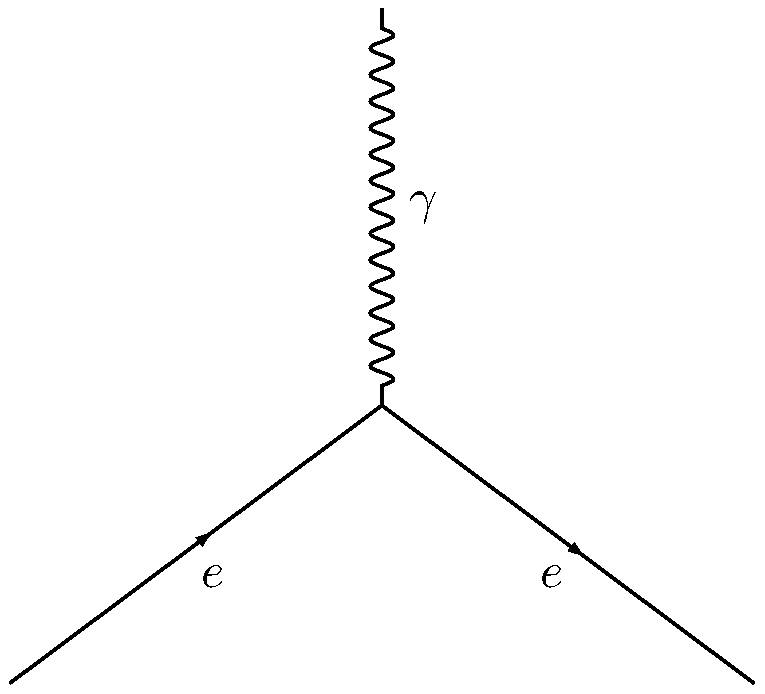
\includegraphics[width=0.25\textwidth]{fig/feynman/forces/qed_vertex.pdf}\label{fig:e_to_ge}}\quad
    \subfloat[$\Pep+\Pem\to\PGg$]{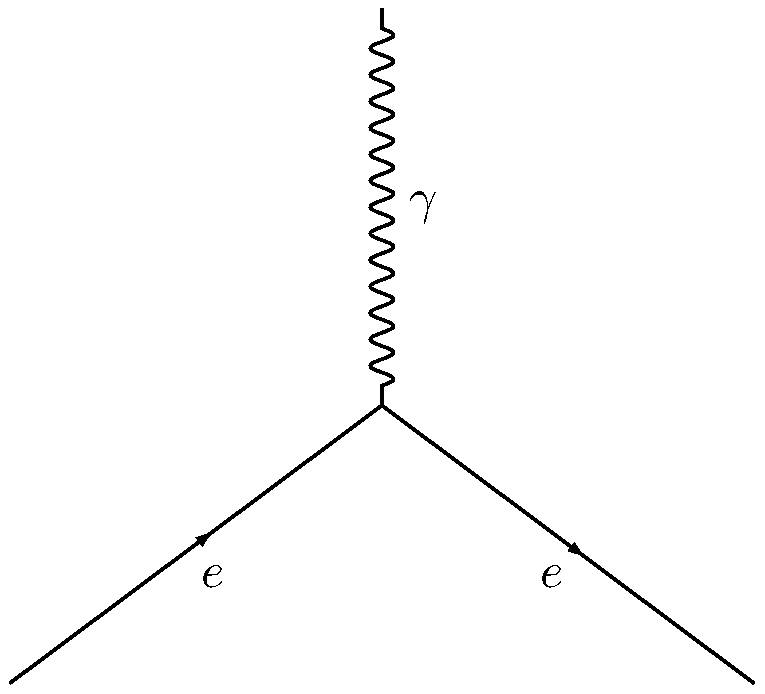
\includegraphics[width=0.25\textwidth]{fig/feynman/forces/qed_vertex.pdf}\label{fig:ee_to_g}}\quad
    \subfloat[$\Pem+\PGg\to\Pem$]{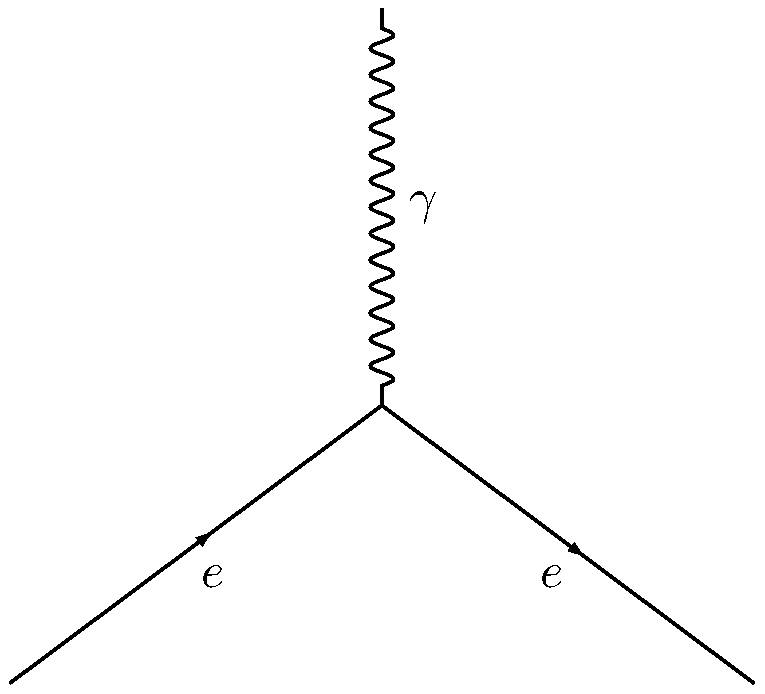
\includegraphics[width=0.25\textwidth]{fig/feynman/forces/qed_vertex.pdf}\label{fig:eg_to_e}}
    \caption{
        Rotations of the QED vertex, showing (a) an electron emitting a photon, (b) an electron and positron annihilating and producing a photon, and (c) an electron absorbing a photon. 
    }
    \label{fig:qed_rotations}
\end{figure}

\begin{figure}[htb]
    \centering
    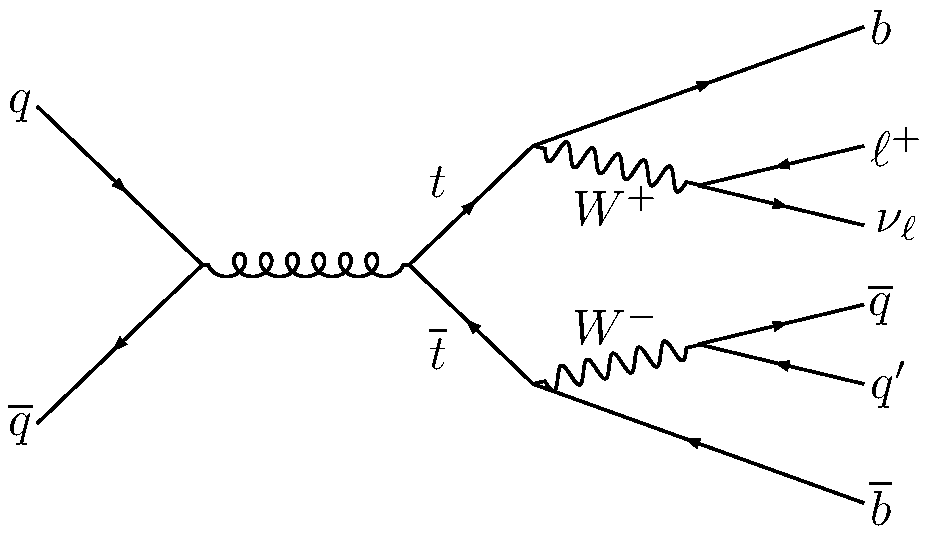
\includegraphics[width=0.6\textwidth]{fig/feynman/ttbar/ttbar_onelep.pdf} % FIXME: missing!!
    \caption{
        Feynman diagram for beta decay, which is mechanism behind the radioactive decay of certain elements. 
    }
    \label{fig:beta_decay}
\end{figure}

\subsection{Cross sections}
Consider two electrons barrelling towards each other with some velocity. 
In the classical picture, the electrons glance off one another and fly off to infinity at some angle to their original trajectories---like two errant ice skaters. 
This can be represented as a Feynman diagram (Fig.~\ref{fig:ee_scattering}) which is assembled from two EM vertices. 
Again, time flows from left to right, showing the two electrons entering, then the exchange of a photon, followed by the two electrons leaving, much like the classical picture. 
Now, suppose we construct two beams of electrons, aim them at each other, then turn them on (preferably after we leave the room). 
In this scenario, we may well want to know the probability that the two electrons will bounce off hach other (``scatter''). 
This probability is called the ``cross section,'' because it is mathematically similar to the classical picture\footnotemark{}, where we would compute the cross-sectional area presented to either of the colliding objects. 
\footnotetext{
    In fact, the answer to this question is expressed in the units of ``barns,'' literally as in ``hitting the broad side of a barn,'' coined by during World War II. % citatin needed
}
Indeed, one of the most important features of QFT is the ability to compute the cross section for scattering two electrons off of each other, as in this case, or any other interactions between particles. 
Feynman diagrams beautifully encode the complex mathematics at work here: each line and every vertex (where three lines meet) correspond a term in the calculation. 
While, again, the mathematical details are beyond the scope of this document, it is important to realize that the Feynman diagram can be directly used to calculate the cross section ($\sigma$):
\begin{equation}
    \sigma = \langle|\mathcal{M}|^2\rangle = \frac{2g_e^4}{(p_1 \cdot p_3)^2(p_1 \cdot p_4)^2[(p_1 \cdot p_2)^4 + (p_1 \cdot p_3)^4 + (p_1 \cdot p_4)^4]}
\end{equation}
where $p_1$ and $p_2$ are the four-momenta of the incoming electrons, $p_3, p_4$ are the four-momenta of the outgoing electrons, and $g_e$ is the EM coupling constant. 
This exercise, and the compact answer above, serves to demonstrate the sheer complexity of QFT calculations. 
Many details were left out beyond the computation itself (which is already a glaring omission), including details surrounding the spin of the electron, the definition of spin, the defition of four-momentum (and special relativity), and so on. 
Those details, and much more, can be found in the illustrious textbook from which this entire example was borrowed~\cite{Griffiths}. 
Moreover, this feature of QFT---the ability to compute cross sections---is absolutely vital because it offers a way of testing the theory with observation: compute the probability that the event is expected to occur, then try to reproduce that event many times in the lab and see how many times it really happens. 

\begin{figure}[htb]
    \centering
    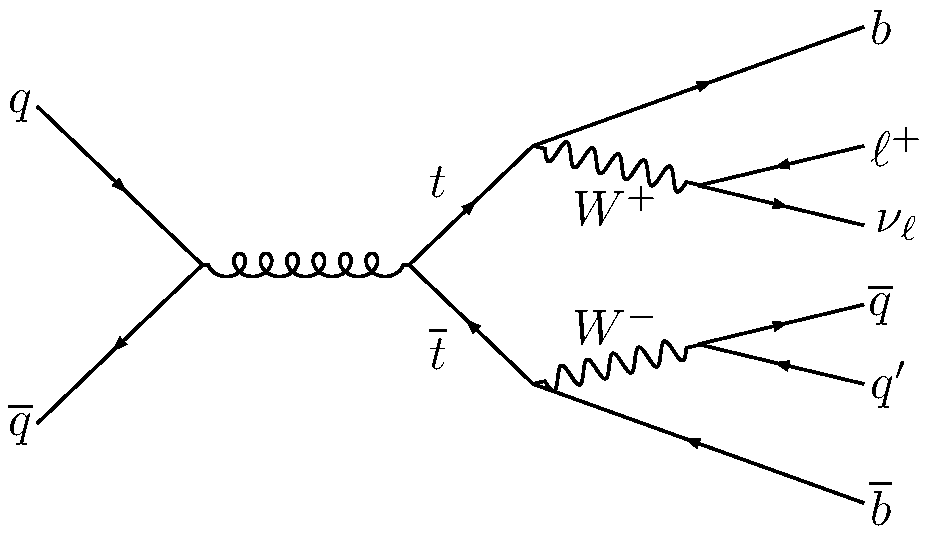
\includegraphics[width=0.6\textwidth]{fig/feynman/ttbar/ttbar_onelep.pdf} % FIXME: missing!!
    \caption{
        Feynman diagram for electron-electron scattering. 
    }
    \label{fig:ee_scattering}
\end{figure}

The validity of any model is a precarious condition: the model must exactly describe reality, else it is not a realization of the truth, but rather only approximately---or worse, accidentally---correct. 
That is, \textit{every} SM cross section value must be accurate for the validity of the model to hold. 
And so generations of physicists have made dilligent, and highly accurate, measurements of a dozens of cross sections---spanning orders of magnitude of rarity. 
Tabulated in grand tables (Fig.~\ref{fig:cms_xsecs} and \ref{fig:atlas_xsecs}), it is evident that the Standard Model has so far withstood every test derived from CMS data and ATLAS data. 
This is an incredible feat: a ``simple'' model seems to describe subatomic physics, which drove the creation of the universe and continues to drive the mechanics of everything, with incredible accuracy. 
Lingering beyond these shining trophies, however, are a number of glaring inconsistencies and enormous missing pieces. 
In other words, we know with certainty that the Standard Model is not complete, and that much more work is needed to complete it. 
We will focus in this dissertation on questions around the Higgs boson, these are detailed in the next section, because these questions motivated the bulk of the work described in the following chapters. 
However, we will also mention some additional open questions to illustrate the magnitude of the problem ahead for future particle physicists. 

\begin{figure}[htb]
    \centering
    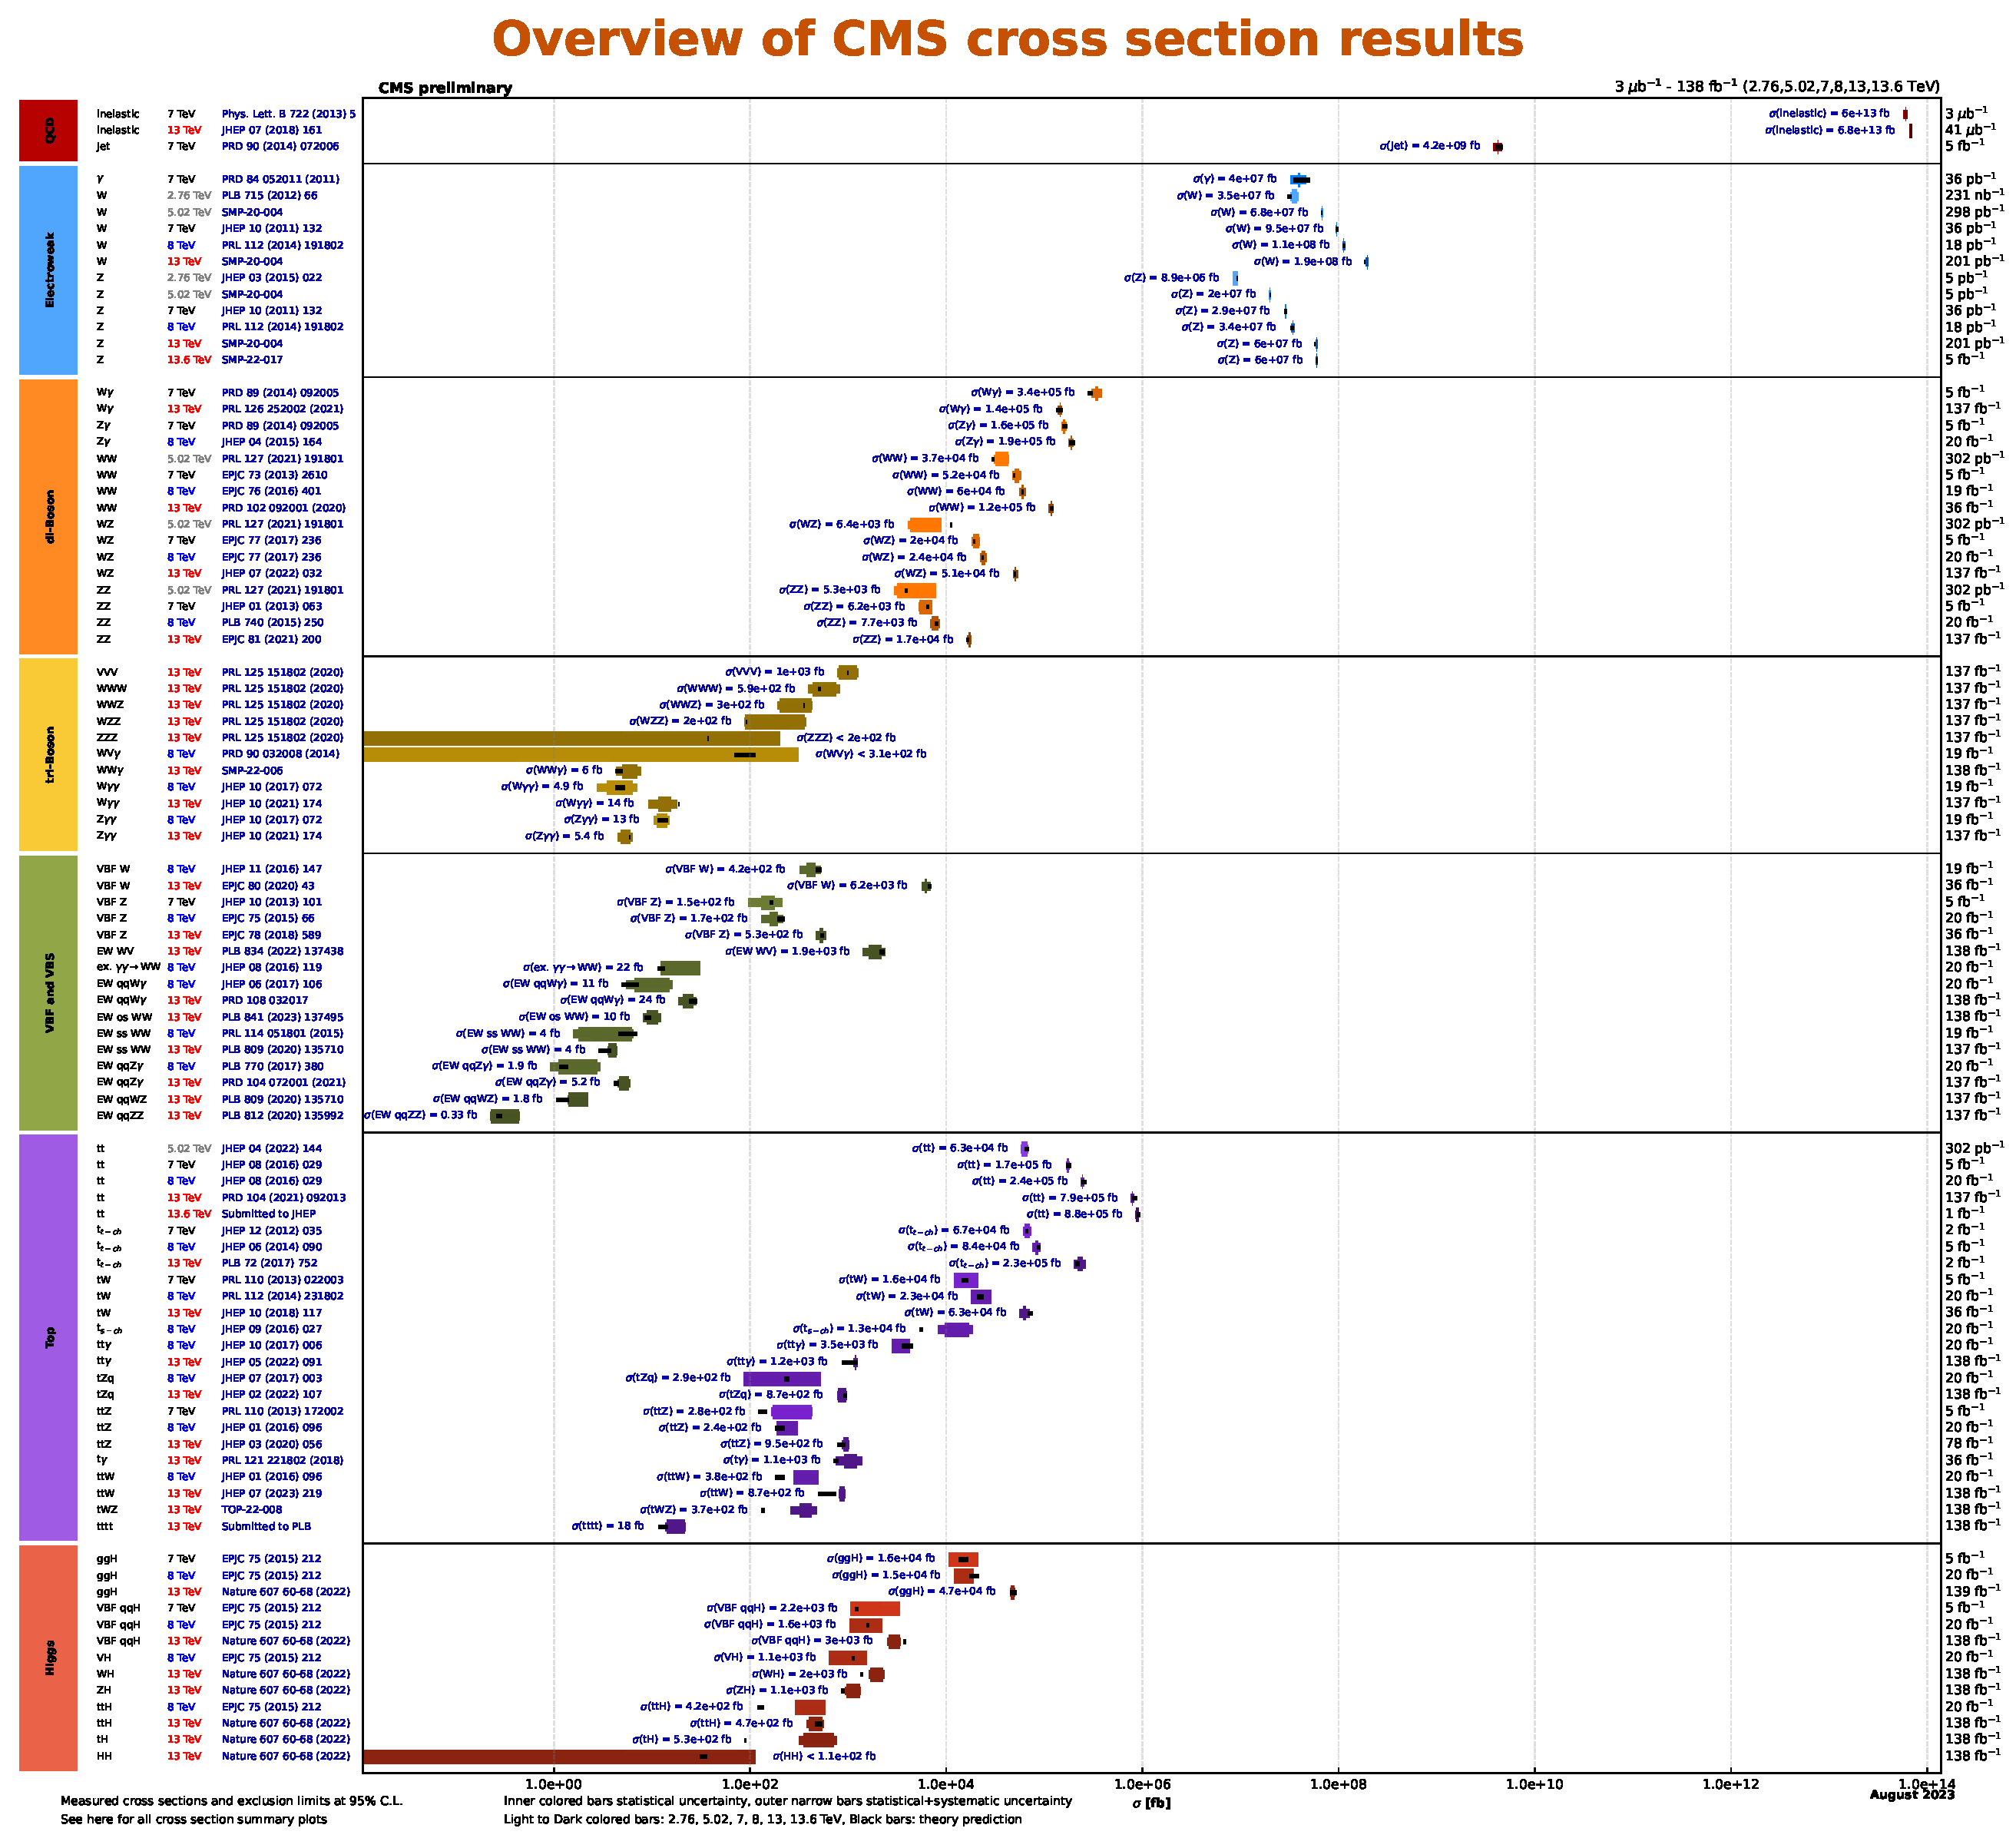
\includegraphics[width=0.9\textwidth]{fig/cms/cms_xsecs_2023.pdf}
    \caption{
        The totality of the cross section measurements performed with data from the CMS Experiment compared to the Standard Model predictions. 
        Precise agreement with the Standard Model can be seen across several orders of magnitude, representing the triumph of the model across decades of experimental scrutiny. 
        Plot taken from Ref.~\cite{CMSXSecs}.
    }
    \label{fig:cms_xsecs}
\end{figure}

\begin{figure}[htb]
    \centering
    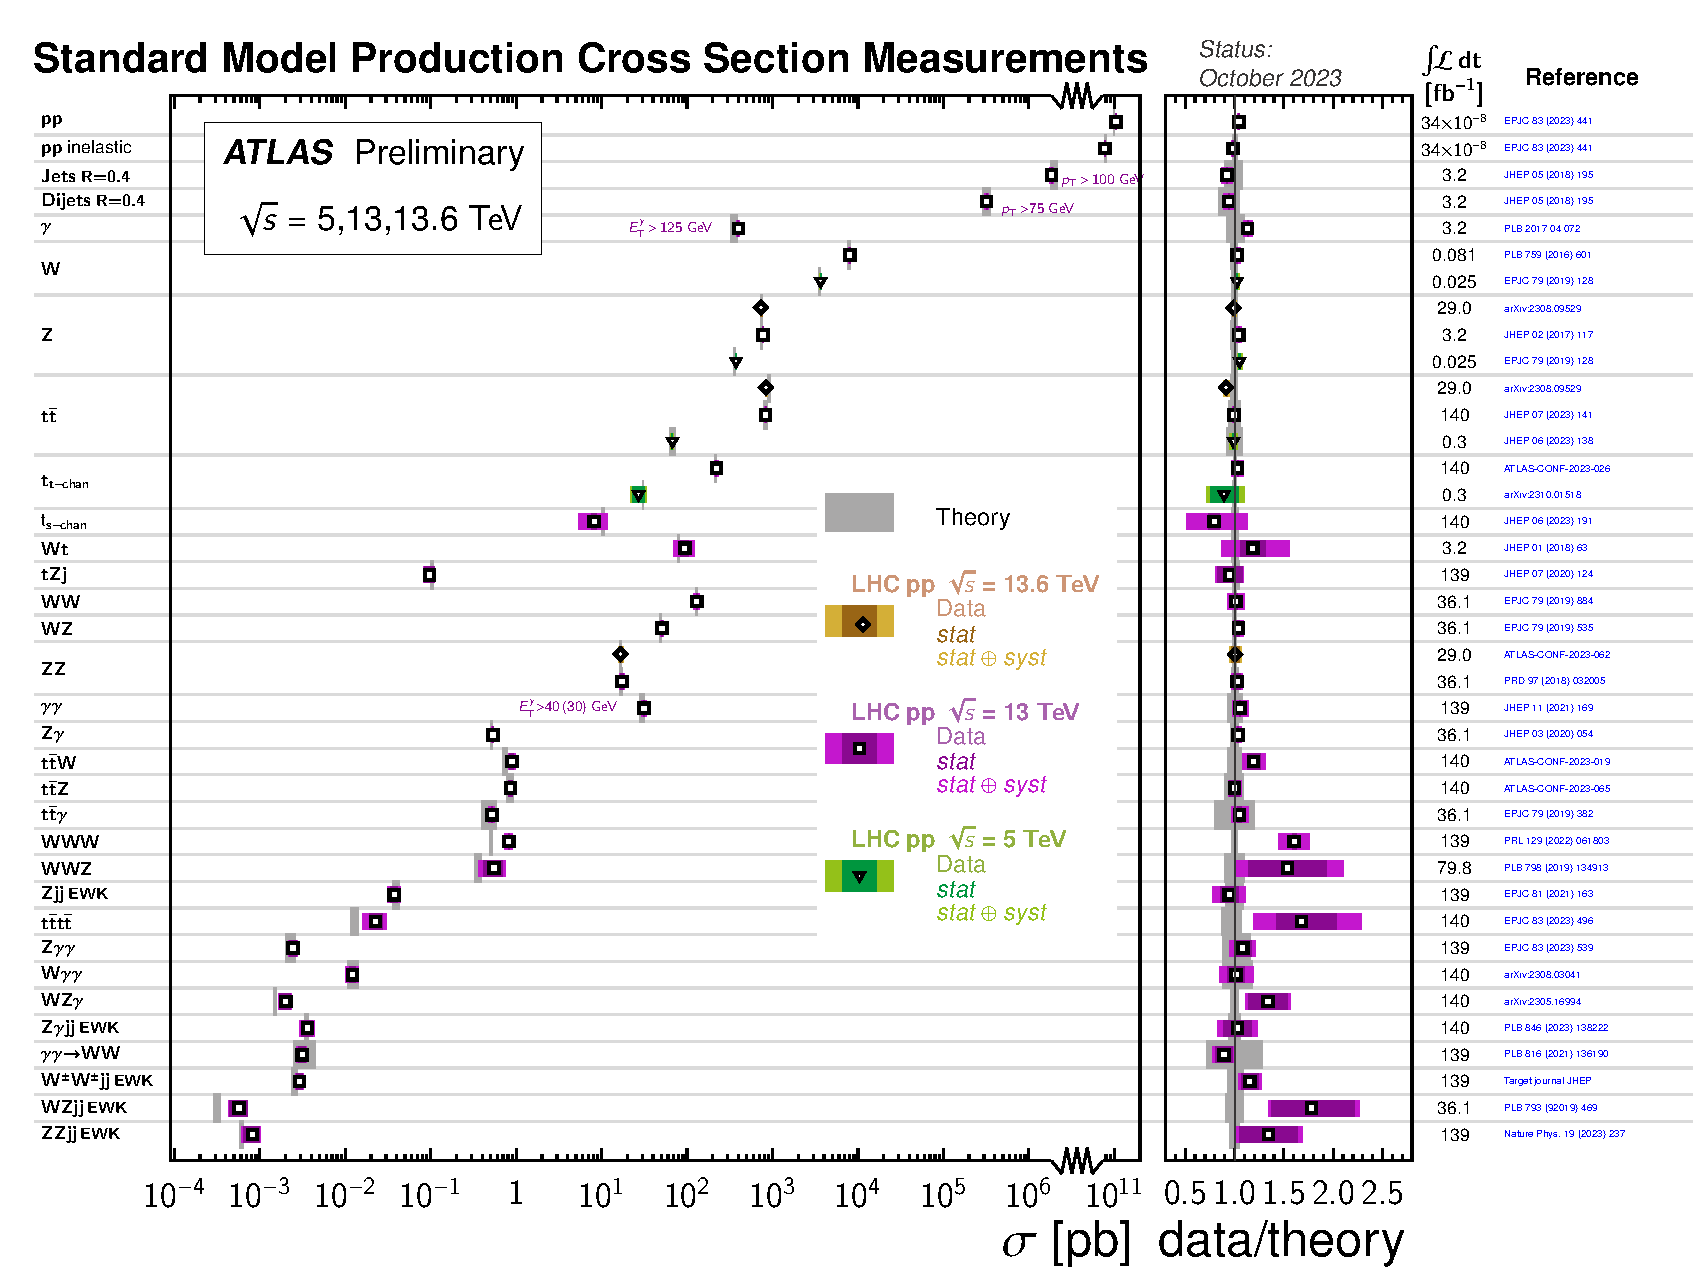
\includegraphics[width=0.9\textwidth]{fig/atlas/atlas_xsecs_2023.pdf}
    \caption{
        A selection of cross section measurements performed with data from the ATLAS Experiment compared to the Standard Model predictions. 
        Precise agreement with the Standard Model can be seen across several orders of magnitude, representing the triumph of the model across decades of experimental scrutiny. 
        Plot taken from Ref.~\cite{ATL-PHYS-PUB-2023-039}.
    }
    \label{fig:atlas_xsecs}
\end{figure}

\subsection{The Higgs boson}
Because we swore to steer away from the details of QFT, we cannot define the Higgs boson and Higgs mechanism completely. 
For this, we are better served by a primer by Griffiths~\cite{Griffiths}, followed by the standard QFT textbooks, and finally the original papers on the subject~\cite{EnglertBroutPRL, HiggsPhysLett, HiggsPRL, GuralnikHagenKibblePRL}. % TODO: add citation for Schroeder, Schredniki, and maybe Schwartz?
Without these prerequisites, it suffices to say that the idea of the Higgs boson is deeply based in Lagrangian mechanics. 
Originally derived for classical systems---an arrow in flight, a planet in motion, a ball on a ramp---an appropriately written ``Lagrangian,'' a mathematical object, together with the Euler-Lagrange equation can reproduce the mathematical description of the dynamics of a given system---the position of the arrow, planets, or ball as a function of time. 
The Lagrangian $L$ is a simple function of the energies in a classical mechanics:
\begin{equation}
    L = \underbrace{\frac{1}{2}m\dot{x}^2}_\text{kinetic energy} - \underbrace{U(x)}_{\substack{\text{potential} \\ \text{energy}}}
\end{equation}
where $x$, really $x(t)$, is the position of some physical object in one direction as a function of time and $\dot{x}$ is shorthand for the derivative of x with respect to time ($\frac{d}{dt}$), or the velocity. 
By plugging $L$ into the Euler-Lagrange equations, we will be able to solve for $x(t)$ with some algebra and calculus: 
\begin{equation}
    \frac{d}{dt}\bigg(\frac{\partial L}{\partial\dot{x}}\bigg) = \frac{\partial L}{\partial x}
\end{equation}

In particle physics, we promote $x(t)$ to a field\footnotemark{} $\phi$, which is a function of space and time $\phi(x, y, z, t)$, and $L$ to $\mathcal{L}$, a Lagrangian \textit{density}.
\footnotetext{Fields are used here in a quantum context, scalar fields in particular, but there are many classical examples: the temperature of a room, the height of the sea, the strength of a magnetic field, these are quantities that may be different at every position in space and may also vary in time.}
Our interest in these abstract fields is well-motivated in QFT, where a field $\phi(x,y,z,t)$ with certain properties corresponds to an observable particle with those same properties. 
For example, the Lagrangian 
\begin{equation}
    \mathcal{L} = \underbrace{\frac{1}{2}(\partial_\mu\phi)(\partial^\mu\phi)}_{\text{kinetic term}} - \underbrace{\frac{1}{2}\big(\frac{mc}{\hbar}\big)^2}_\text{mass term}
\end{equation}
represents a spin-0 particle with mass $m$. 
As in classical machanics, plugging the appropriate Lagrangian density into the Euler-Lagrange equation yields the precise descriptions of the dynamics of fundamental particles. 

The Higgs mechanism arises when we try to write down a Lagrangian density $\mathcal{L}$ that accounts for the existence of the $\PW$ and $\PZ$ bosons. % for some reason, $$ are needed here, else the doc breaks
In doing so, we find that we must demand that $\mathcal{L}$ does not change under certain transformations of the fields $\phi$, which, at face value, equates to demanding that the field is massless---without going into details, this claim must simply be accepted as true. 
This is a problem because the $\PW$ and $\PZ$ bosons are verifiably not massless. % for some reason, $$ are needed here, else the doc breaks
However, by introducing two scalar fields---corresponding to the Higgs boson and Goldstone boson---and massaging the mathematics, a mass term emerges for the $\PW$ and $\PZ$ bosons. % for some reason, $$ are needed here, else the doc breaks
The Goldstone boson does not correspond to a real particle, but instead services the mathematics\footnotemark{} and disappears under a specific transformation. 
\footnotetext{For example, it accounts for the fact that there are three bosons that carry the weak force ($\PW^{+}$, $\PW^{-}$, $\PZ$).} % for some reason, $$ are needed here, else the doc breaks
The Higgs \textit{mechanism} itself refers to the appearance of the $\PW$ and $\PZ$ boson masses, as well as the fermion masses through different interactions~\cite{Weinberg:1967tq, Nambu:1961fr}. % for some reason, $$ are needed here, else the doc breaks

Beyond the blackboard, the Higgs mechanism gives us a picture of how the universe came to be: in the first moments of time, the fundamental particles were endowed with mass by the Higgs mechanism. 
Thus, rather than fly off to infinity at the speed of light, atoms were formed, and the universe as we know it bloomed.  
The Higgs boson is therefore essential to the origin and continued existence of the known universe---in fact, if the Higgs field were to spontaneously dissappear, the entire universe would evaporate in a nanosecond. % citation needed
It is also, however, a key to understanding the universe's distant future~\cite{Bass2021}: will the universe collapse or explode or something else entirely? % citation needed
We shall spare ourselves of existential crisis and instead simply appreciate the specific importance of the Higgs boson. 
While every piece of the Standard Model is important, just as every link in a chain, the Higgs boson is one of the less well-understood particles, and further study of this latest addition to the Standard Model may shed crucial light on the many open questions in particle physics. 

\section{Selected open questions}\label{sec:open_questions}
\subsection{What is dark matter?}
\subsection{What is dark energy?}
\subsection{Is the Higgs boson really a fundamental particle?}
\subsection{Is there only one Higgs boson?}
\subsection{Why is the Higgs boson mass so small?}
% Higgs sector:
%    - naturalness?
%    - other higgses?? Gell-Mann said something like "it would be weird if 
%      there was only one Higgs boson" in 2012 CERN interview
%    - other problems... I guess introduce problem of not yet measuring 
%      higgs couplings well
% More generic:
%    - dark matter

\chapter{A Grand Apparatus}\label{ch:lhc_cms}
\begin{aquote}{Fran\c{c}ois Englert, CMS: The Art of Science, 2016}
    A glance at the ATLAS and CMS detectors at CERN reveals their beauty...
    These detectors are the modern cathedrals of the rational world created by scientists, experimentalists, and theoreticians. 
\end{aquote}

\section{The Large Hadron Collider}
The Large Hadron Collider (LHC) is the largest particle accelerator ever built. 
Its most striking feature is a 27 km ring buried 100 m beneath the Franco-Swiss border (Fig.~\ref{fig:lhc_depth}) in which two beams of protons (or heavy ions like lead), after going through several smaller stages (Fig.~\ref{fig:cern_complex}), are accelerated to 99.9999991\% of the speed of light in opposite directions. 
The beams are steered by thousands of magnets, including 1232 superconducting dipole magnets (Fig.~\ref{fig:lhc_dipole}), placed along the circumference of the ring. 
At various points, the proton beams are directed towards each other, allowing the protons to collide. 
These collision points are surrounded by enormous, multi-layered particle detectors which record snapshots of the collisions. 

\begin{figure}[htb]
    \centering
    \subfloat{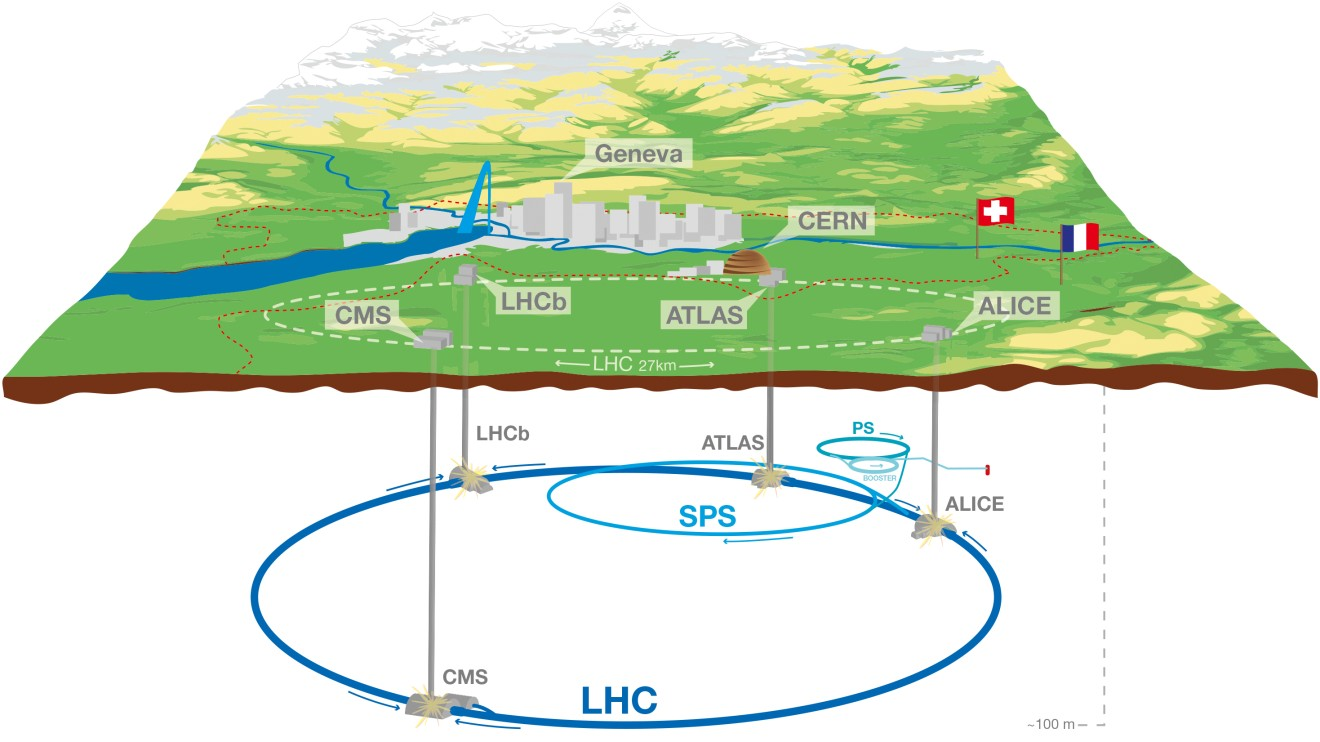
\includegraphics[width=0.45\textwidth,valign=c]{fig/lhc/lhc_depth.jpg}}\quad
    \subfloat{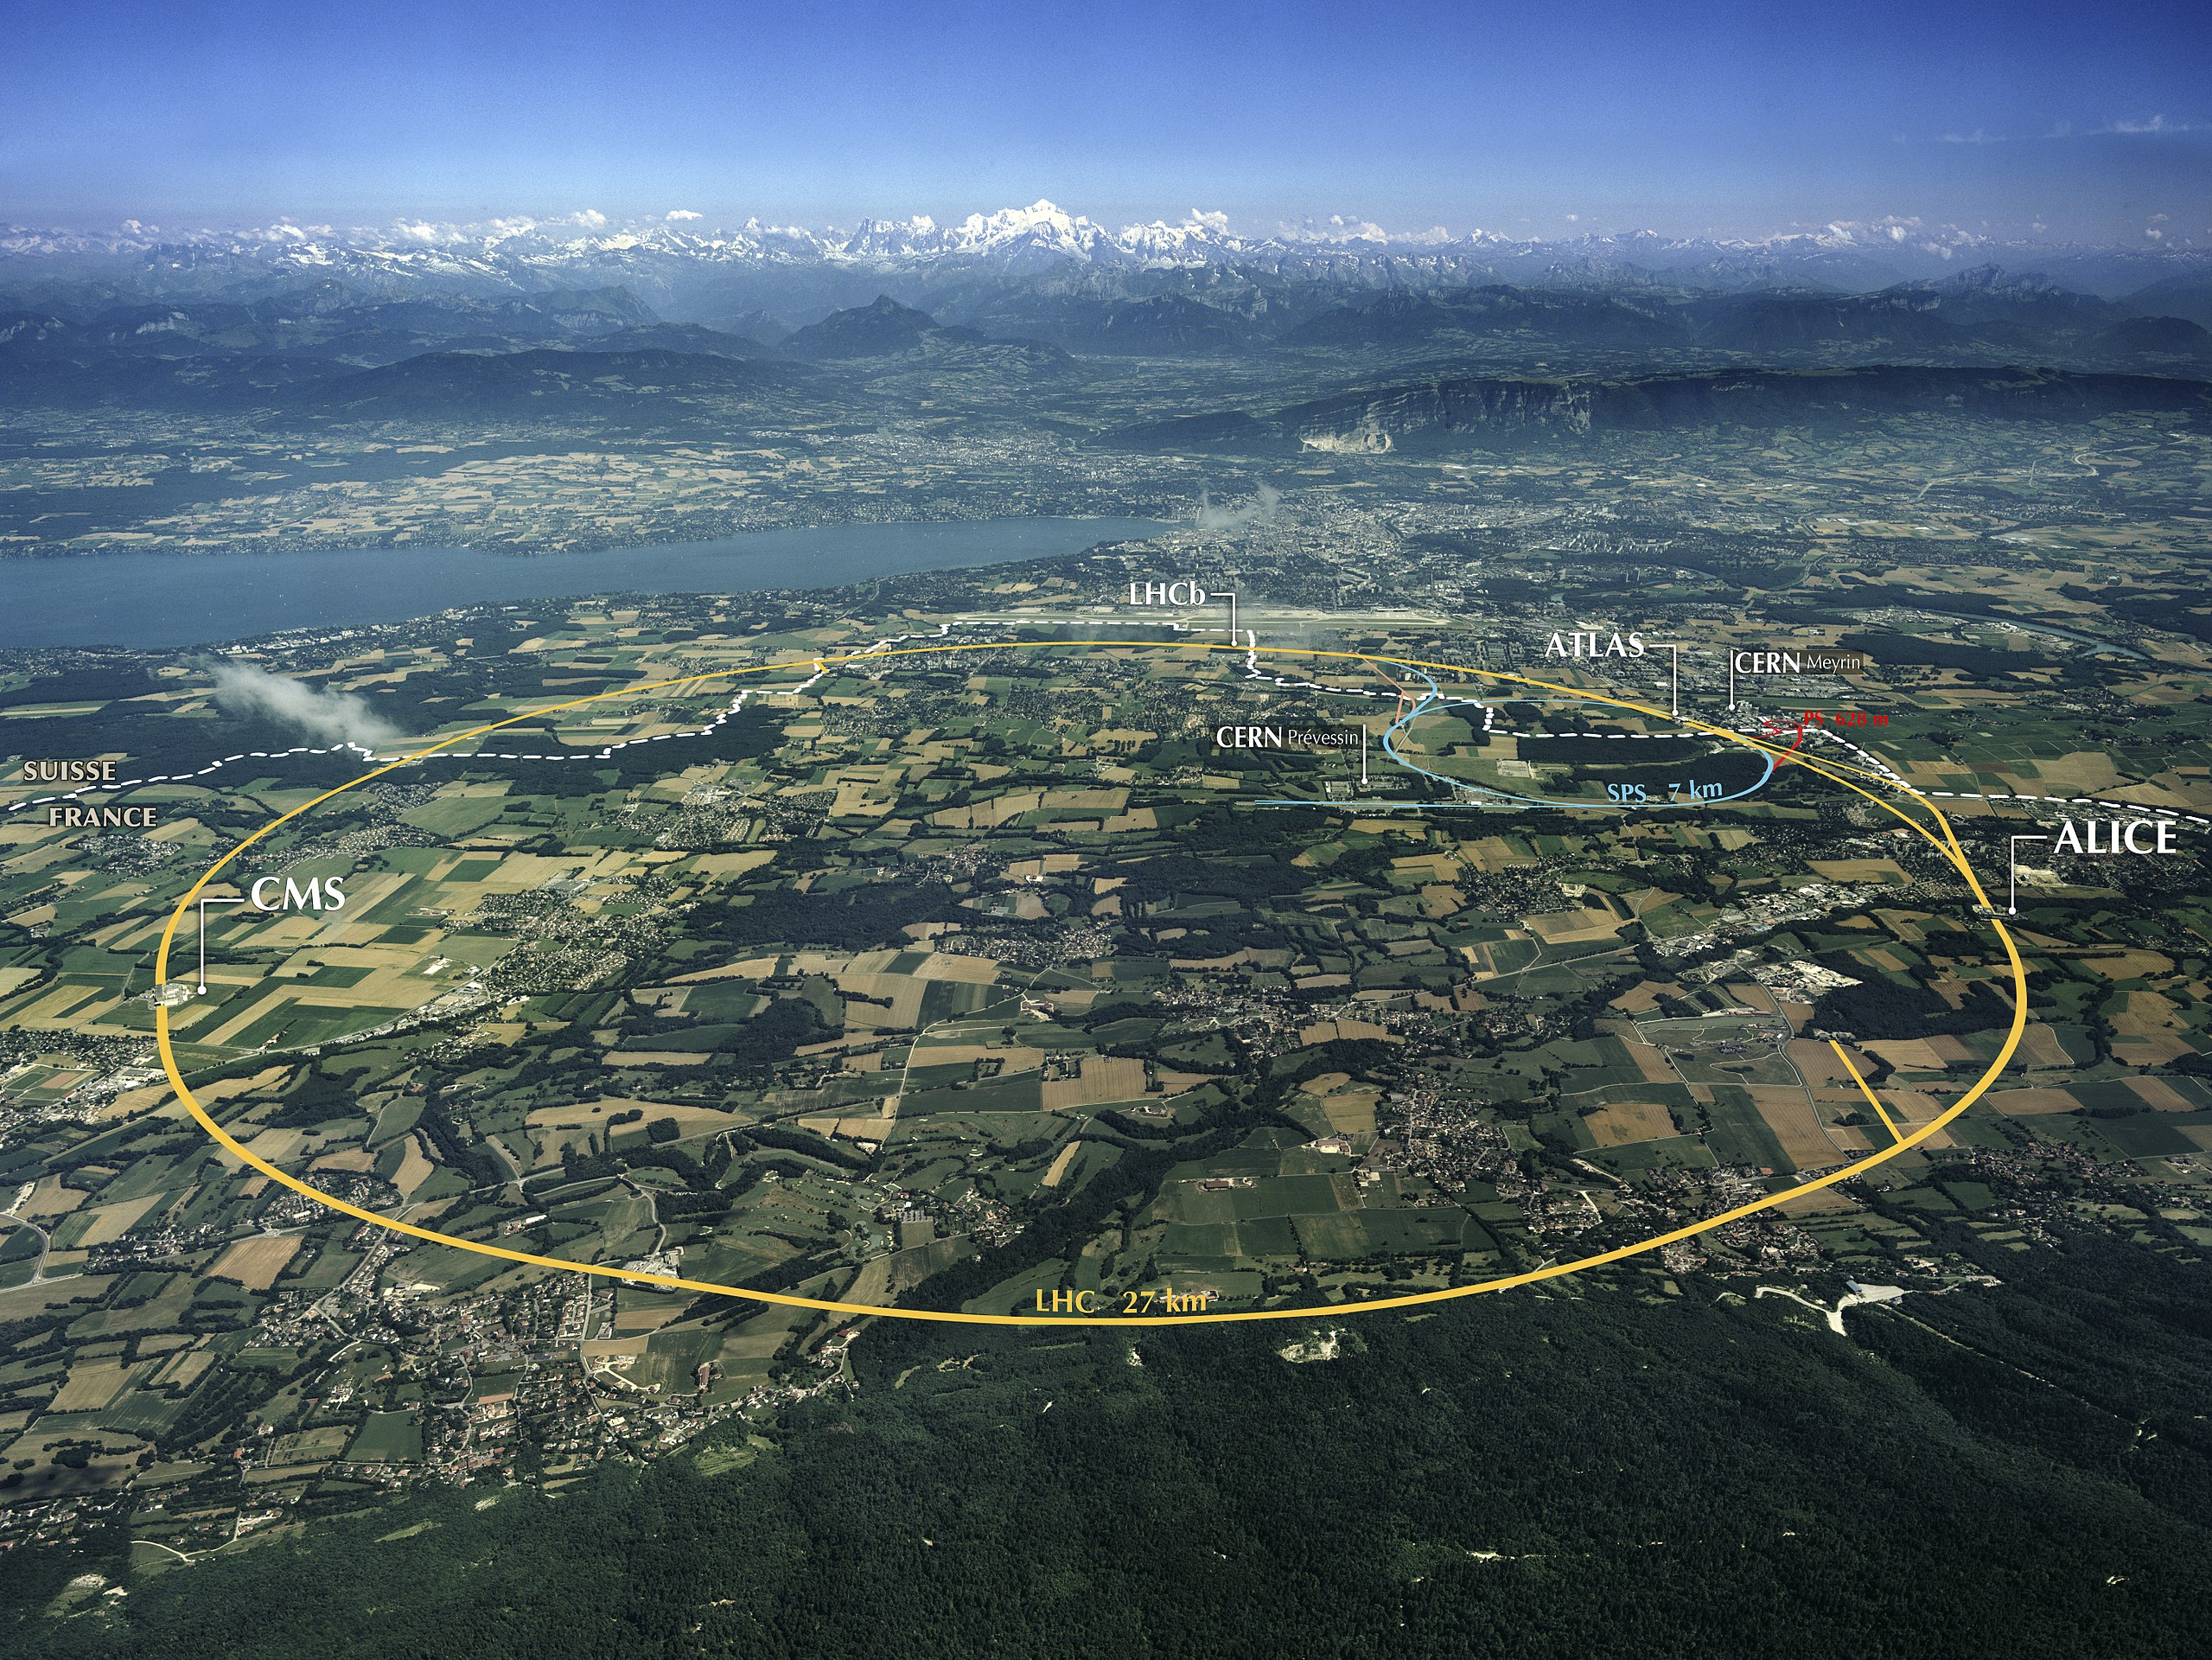
\includegraphics[width=0.45\textwidth,valign=c]{fig/lhc/cern_aerial_view.jpg}}
    \caption{
        A diagram illustrating the depth of the LHC beneath the surface (left), from Ref.~\cite{Servicegraphique:1708849}, and an aerial photograph of the entire CERN complex (right), from Ref.~\cite{Maximilien:1295244}. 
        The SPS and LHC tunnels illustrated in both figures. 
    }
    \label{fig:lhc_depth}
\end{figure}

\begin{figure}[htb]
    \centering
    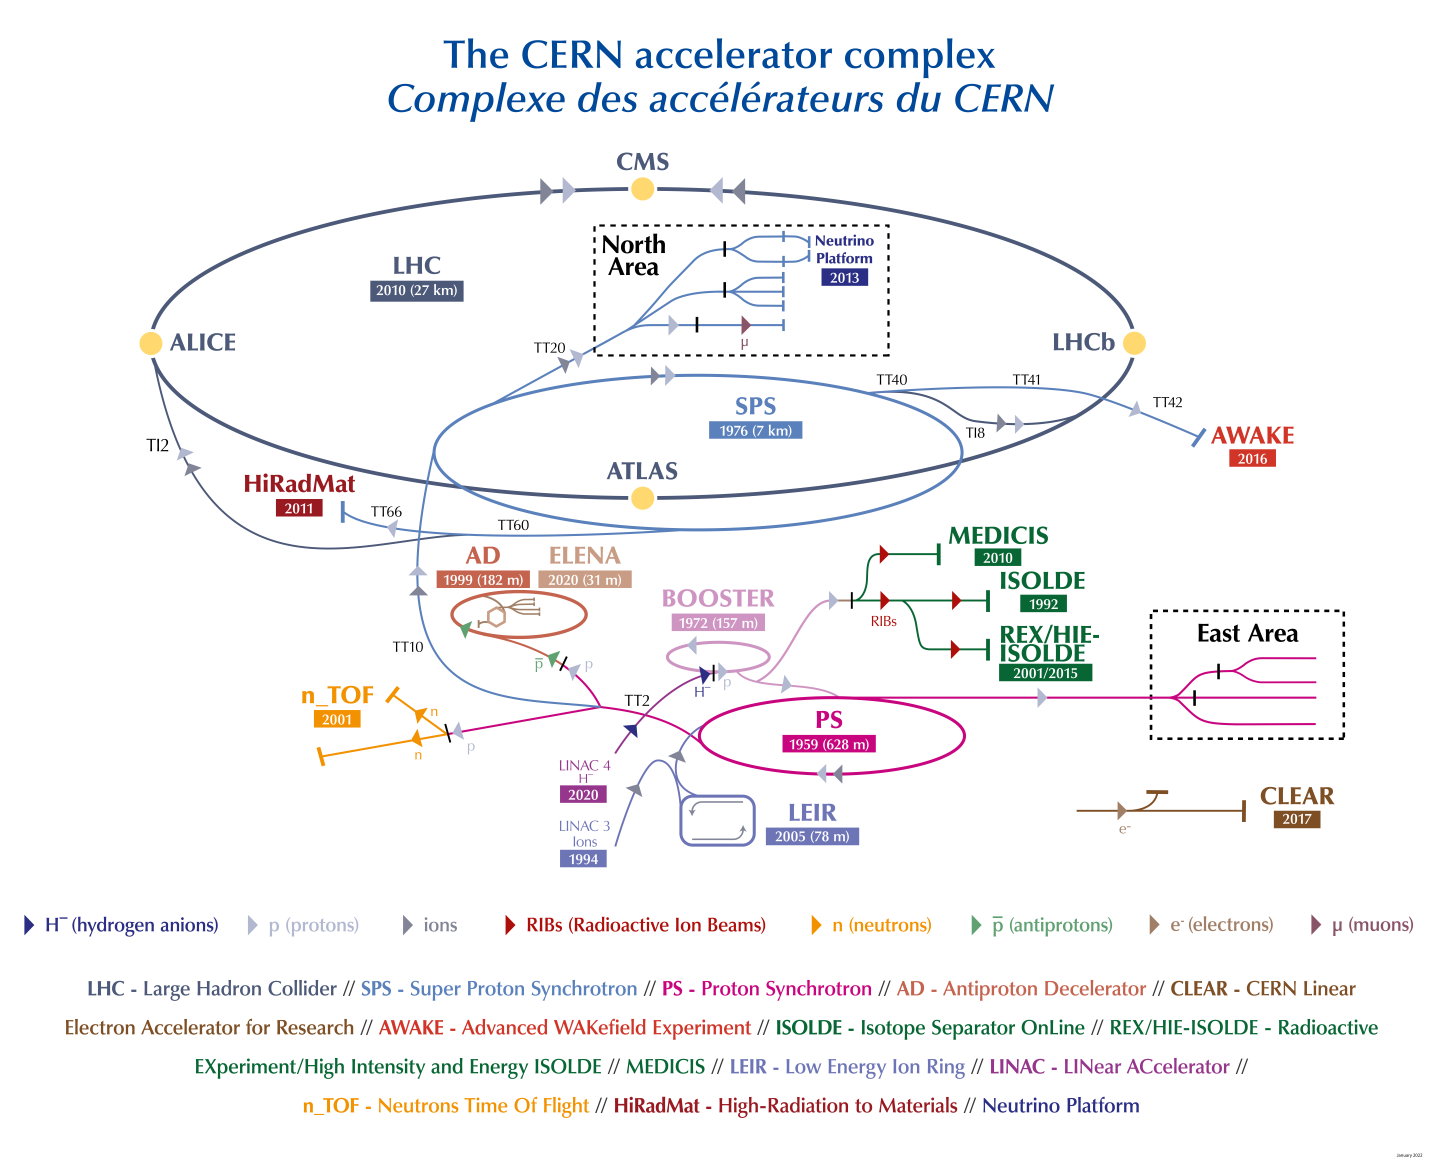
\includegraphics[width=0.95\textwidth]{fig/lhc/lhc_complex.png}
    \caption{
        The CERN complex illustrated in detail, from Ref.~\cite{Lopienska:2800984}. 
        The different stages of particle acceleration can be seen in detail, described here for protons. 
        First, negative hydrogen ions (H$^-$) generated by LINAC 4 are fed into BOOSTER, which strips the electrons from the H$^-$ ions, leaving only the protons, and accelerates them to 2\GeV. 
        Next, the Proton Synchrotron (PS) accelerates the protons to 26\GeV. 
        The PS feeds into the Super Proton Synchrotron (SPS) which further accelerates them to to 450\GeV. 
        Finally, the protons are fed into the LHC, which accelerates them to a final energy of 7\TeV. 
    }
    \label{fig:cern_complex}
\end{figure}

\begin{figure}[htb]
    \centering
    \subfloat{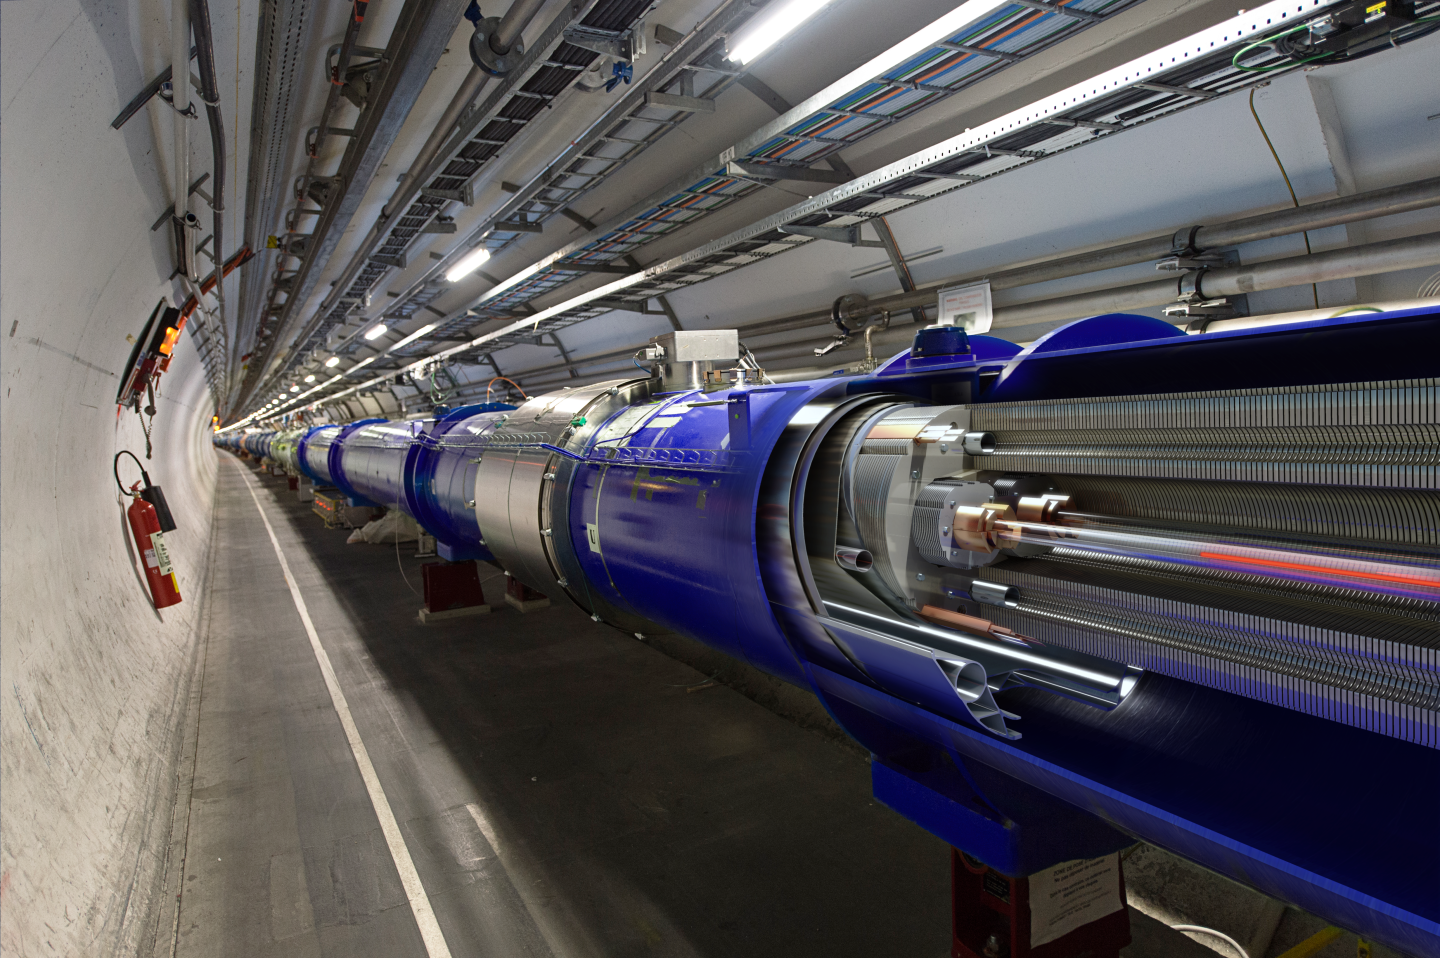
\includegraphics[width=0.475\textwidth,valign=c]{fig/lhc/dipole_cutaway.png}}\quad
    \subfloat{\includegraphics[width=0.425\textwidth,valign=c]{fig/lhc/dipole_jguiang.png}}
    \caption{
        A cutaway diagram illustrating the internals of a dipole magnet inside the LHC tunnel (left), from Ref.~\cite{Dominguez:1741036}, and a photograph of a decomissioned dipole magnet with a physicist for scale (right).
    }
    \label{fig:lhc_dipole}
\end{figure}

The protons are accelerated in bunches, composed of approximately 115 billion protons each, so when the bunches are brought together (called a ``bunch crossing''), over 200 billion protons are brought very close together.
However, only a small portion of them actually collide. 
During ``Run 2'' of the LHC from 2016 to 2018, for instance, there were 30 proton-proton (pp) collisions (e.g. Fig.~\ref{fig:normal_pu}) per bunch crossing on average, typically with only a single ``interesting'' collision (the ``primary vertex'') amongst them. % TODO: citation needed, plot or something of pileup needed
A collision is deemed interesting if it initiates a process that a physicist at the LHC wants to study (e.g. Fig.~\ref{fig:vbswh_feynman})---the non-interesting collisions are called ``pileup.'' 
To increase our odds of producing something truly interesting, the bunch crossings are spaced close together, with only 25 nanoseconds of separation. 
To put this into context, the speed of light is roughly 1 ft/ns, so the next bunch crossing will occur before the light from a screen on one side of the CMS control room can reach the eyes of someone standing on the other side (approximately 39 feet~\cite{CMSP5Layout}).
Therefore, particle detectors on the LHC must be capable of excellent resolution \textit{and} high throughput. 
That is, they must be able to resolve the particles from the primary vertex amongst the many others produced by the pileup, all within the 25 ns between bunch crossings. 

\subsection{Collision energy}
The collision energy, often written as $\sqrt{s}$, is measured in electronvolts (eV), the standard unit of energy in particle physics---more specifically, teraelectronvolts (TeV), or trillions of eV. 
In Run I of the LHC (2011--2012) the collision energy was ramped up to a maximum of 8\TeV, much lower than what the LHC was designed for. % TODO: citation needed
This was done out of an abundance of caution due to the fact that the LHC exploded when it was first turned on in 2008. % TODO: citation needed
Then, in Run II (2016--2018), the collision energy was increased to 13\TeV. 
Over the course of Run III, the collision energy will be ramped up to 14\TeV, where it will be held for the remainder of the LHC's lifetime (Fig.~\ref{fig:hl_lhc_timeline}). 

\subsection{Luminosity}
The luminosity ($\Lumi$) is measured in the inverse of the units of a cross section---inverse femptobarns ($\fbinv$), in particular. 
This allows for a quick calculation of how many pp collisions one can expect: simply multiply the lumonisity by the pp inelastic scattering cross section. 

\clearpage

\section{The Compact Muon Solenoid}
The Compact Muon Solenoid (CMS) Experiment is one of two general purpose LHC experiments, the other being the ATLAS\footnotemark{} Experiment, among the four major experiments supported by the LHC~\cite{LHCWeb}, where the other two are more specialized: ALICE, for studying heavy ion collisons, and LHCb, for studying b quarks. 
\footnotetext{Whereas ATLAS is, putting it politely, a rather creative acronym: ``A Toroidal LHC ApparatuS.''}
Compared to ATLAS, which stands at a mighty $46\times25\times25$ meters in dimension, CMS is ``compact'' at a stout $21\times15\times15$ m, with a dedicated muon system and one of the world's largest solenoid magnets~\cite{ATLASWeb, CMSWeb}. 
See Fig.~\ref{fig:cms_labeled} for its exact specifications, and Figures~\ref{fig:cms_pics} and \ref{fig:cms_jguiang} for some beauty shots. 

\begin{figure}[htb]
    \centering
    \includegraphics[width=0.9\textwidth]{fig/cms/cms_labeled.jpg}
    \caption{
        A detailed cutaway diagram of CMS, with each subdetector labeled with its name and some its characteristics, from Ref.~\cite{Sakuma:2665537}. 
    }
    \label{fig:cms_labeled}
\end{figure}

\begin{figure}[htb]
    \centering
    \subfloat{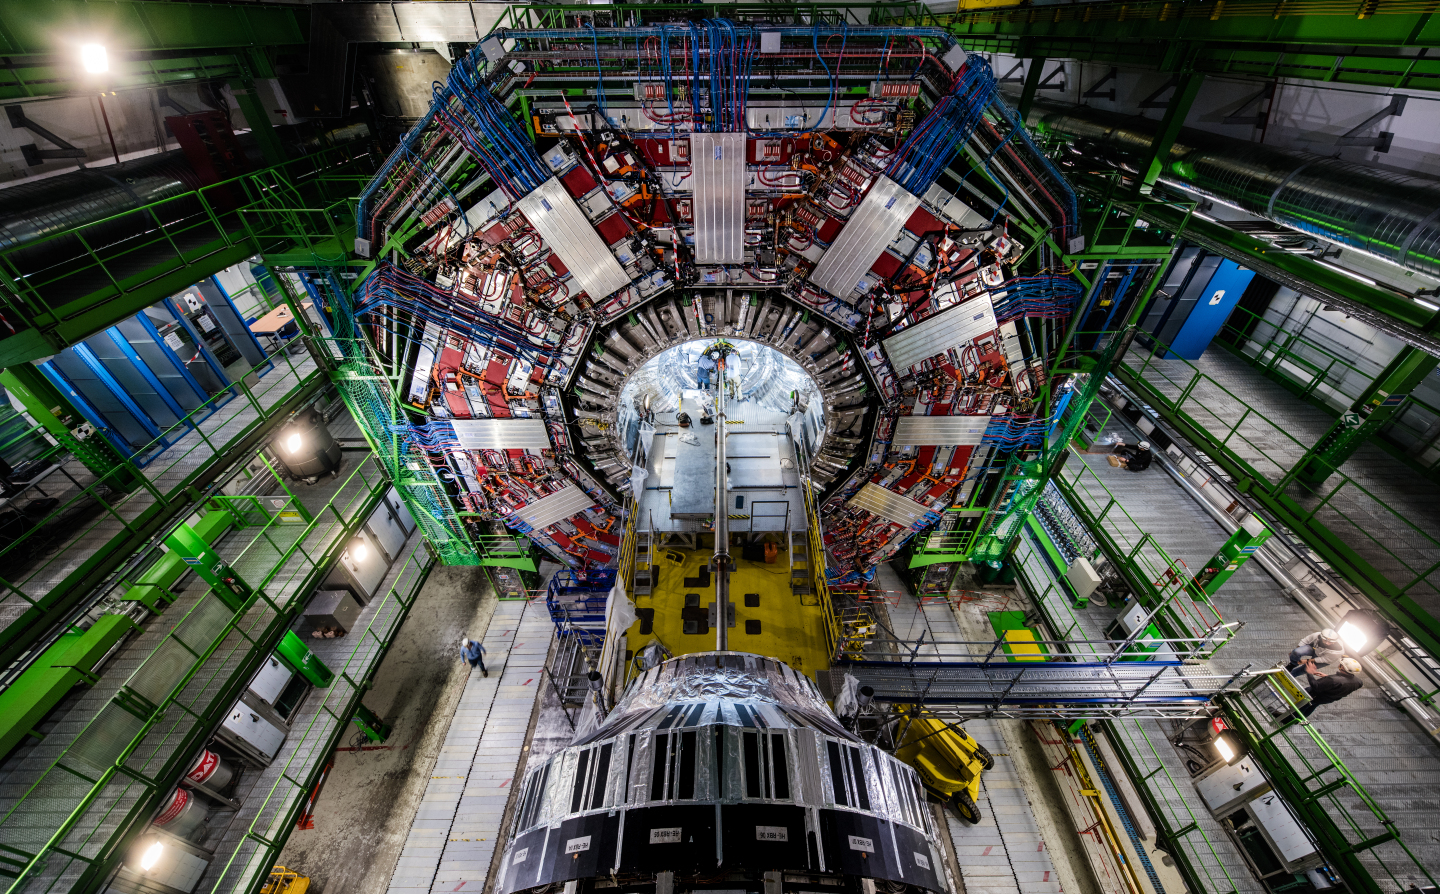
\includegraphics[width=0.465\textwidth]{fig/cms/cms_picture1.jpg}}\quad
    \subfloat{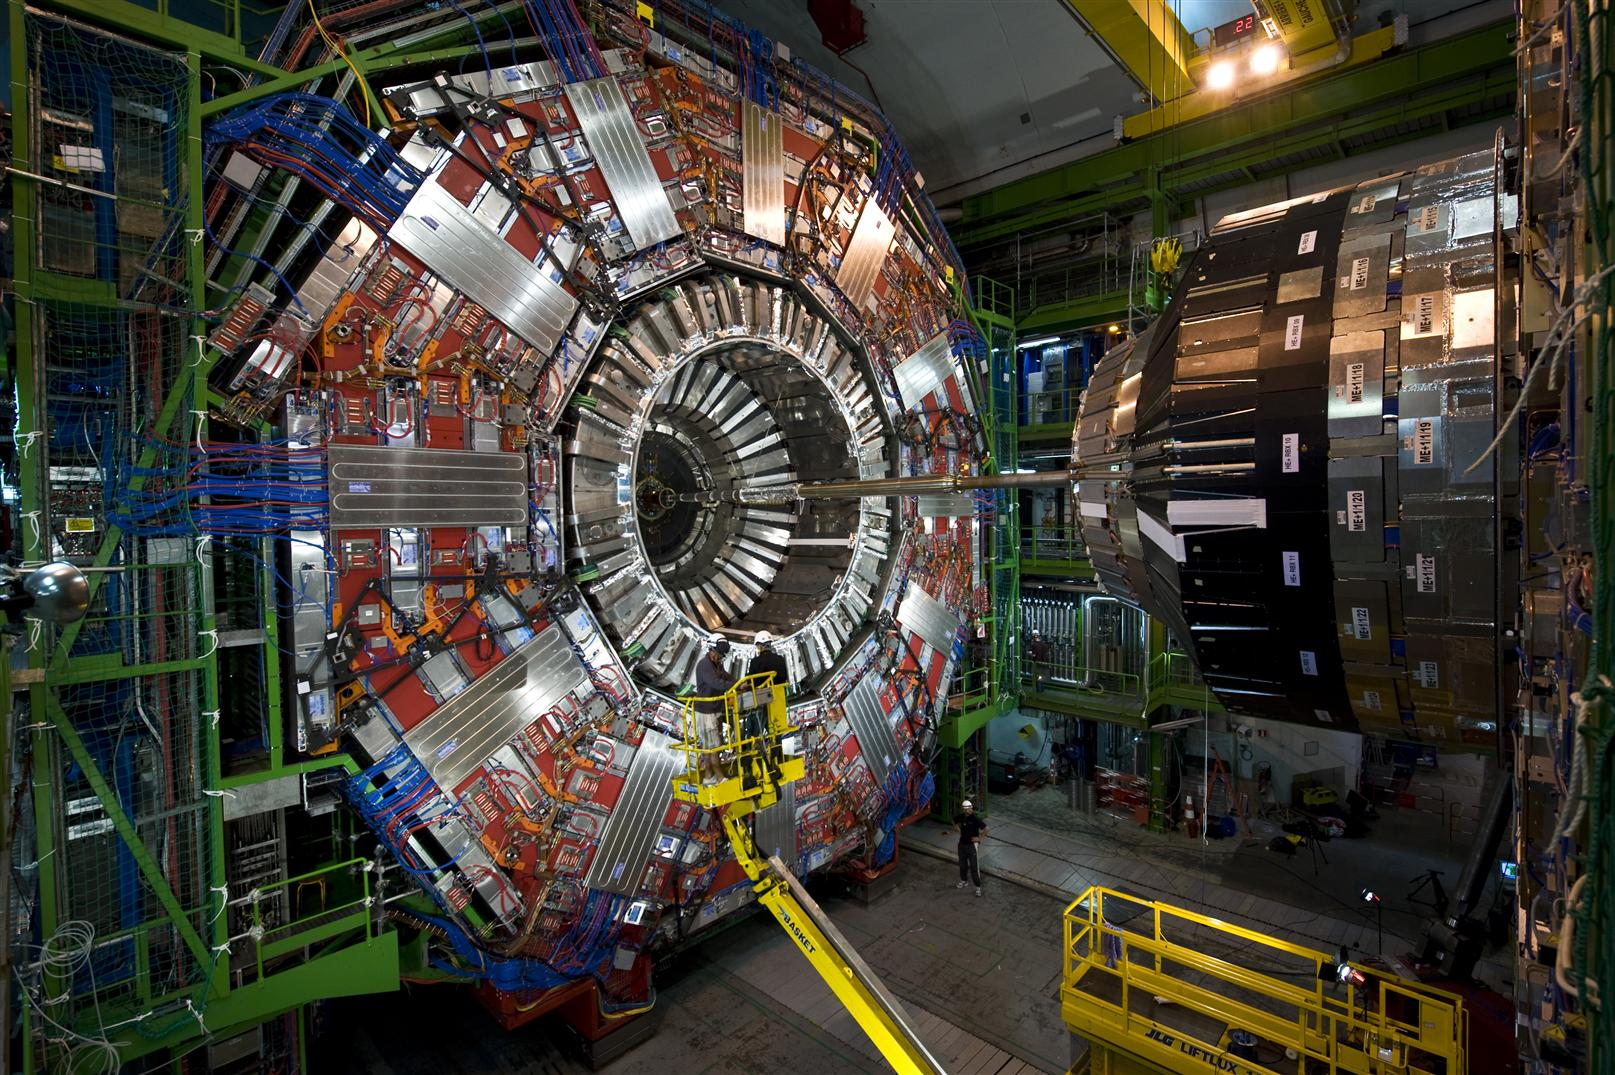
\includegraphics[width=0.435\textwidth]{fig/cms/cms_picture2.jpg}}
    \caption{
        The Compact Muon Solenoid in all of its glory, with one of the endcaps separated from the main body of the experiment, pictured from the top (left) and side (right). 
    }
    \label{fig:cms_pics}
\end{figure}

\begin{figure}[htb]
    \centering
    \subfloat{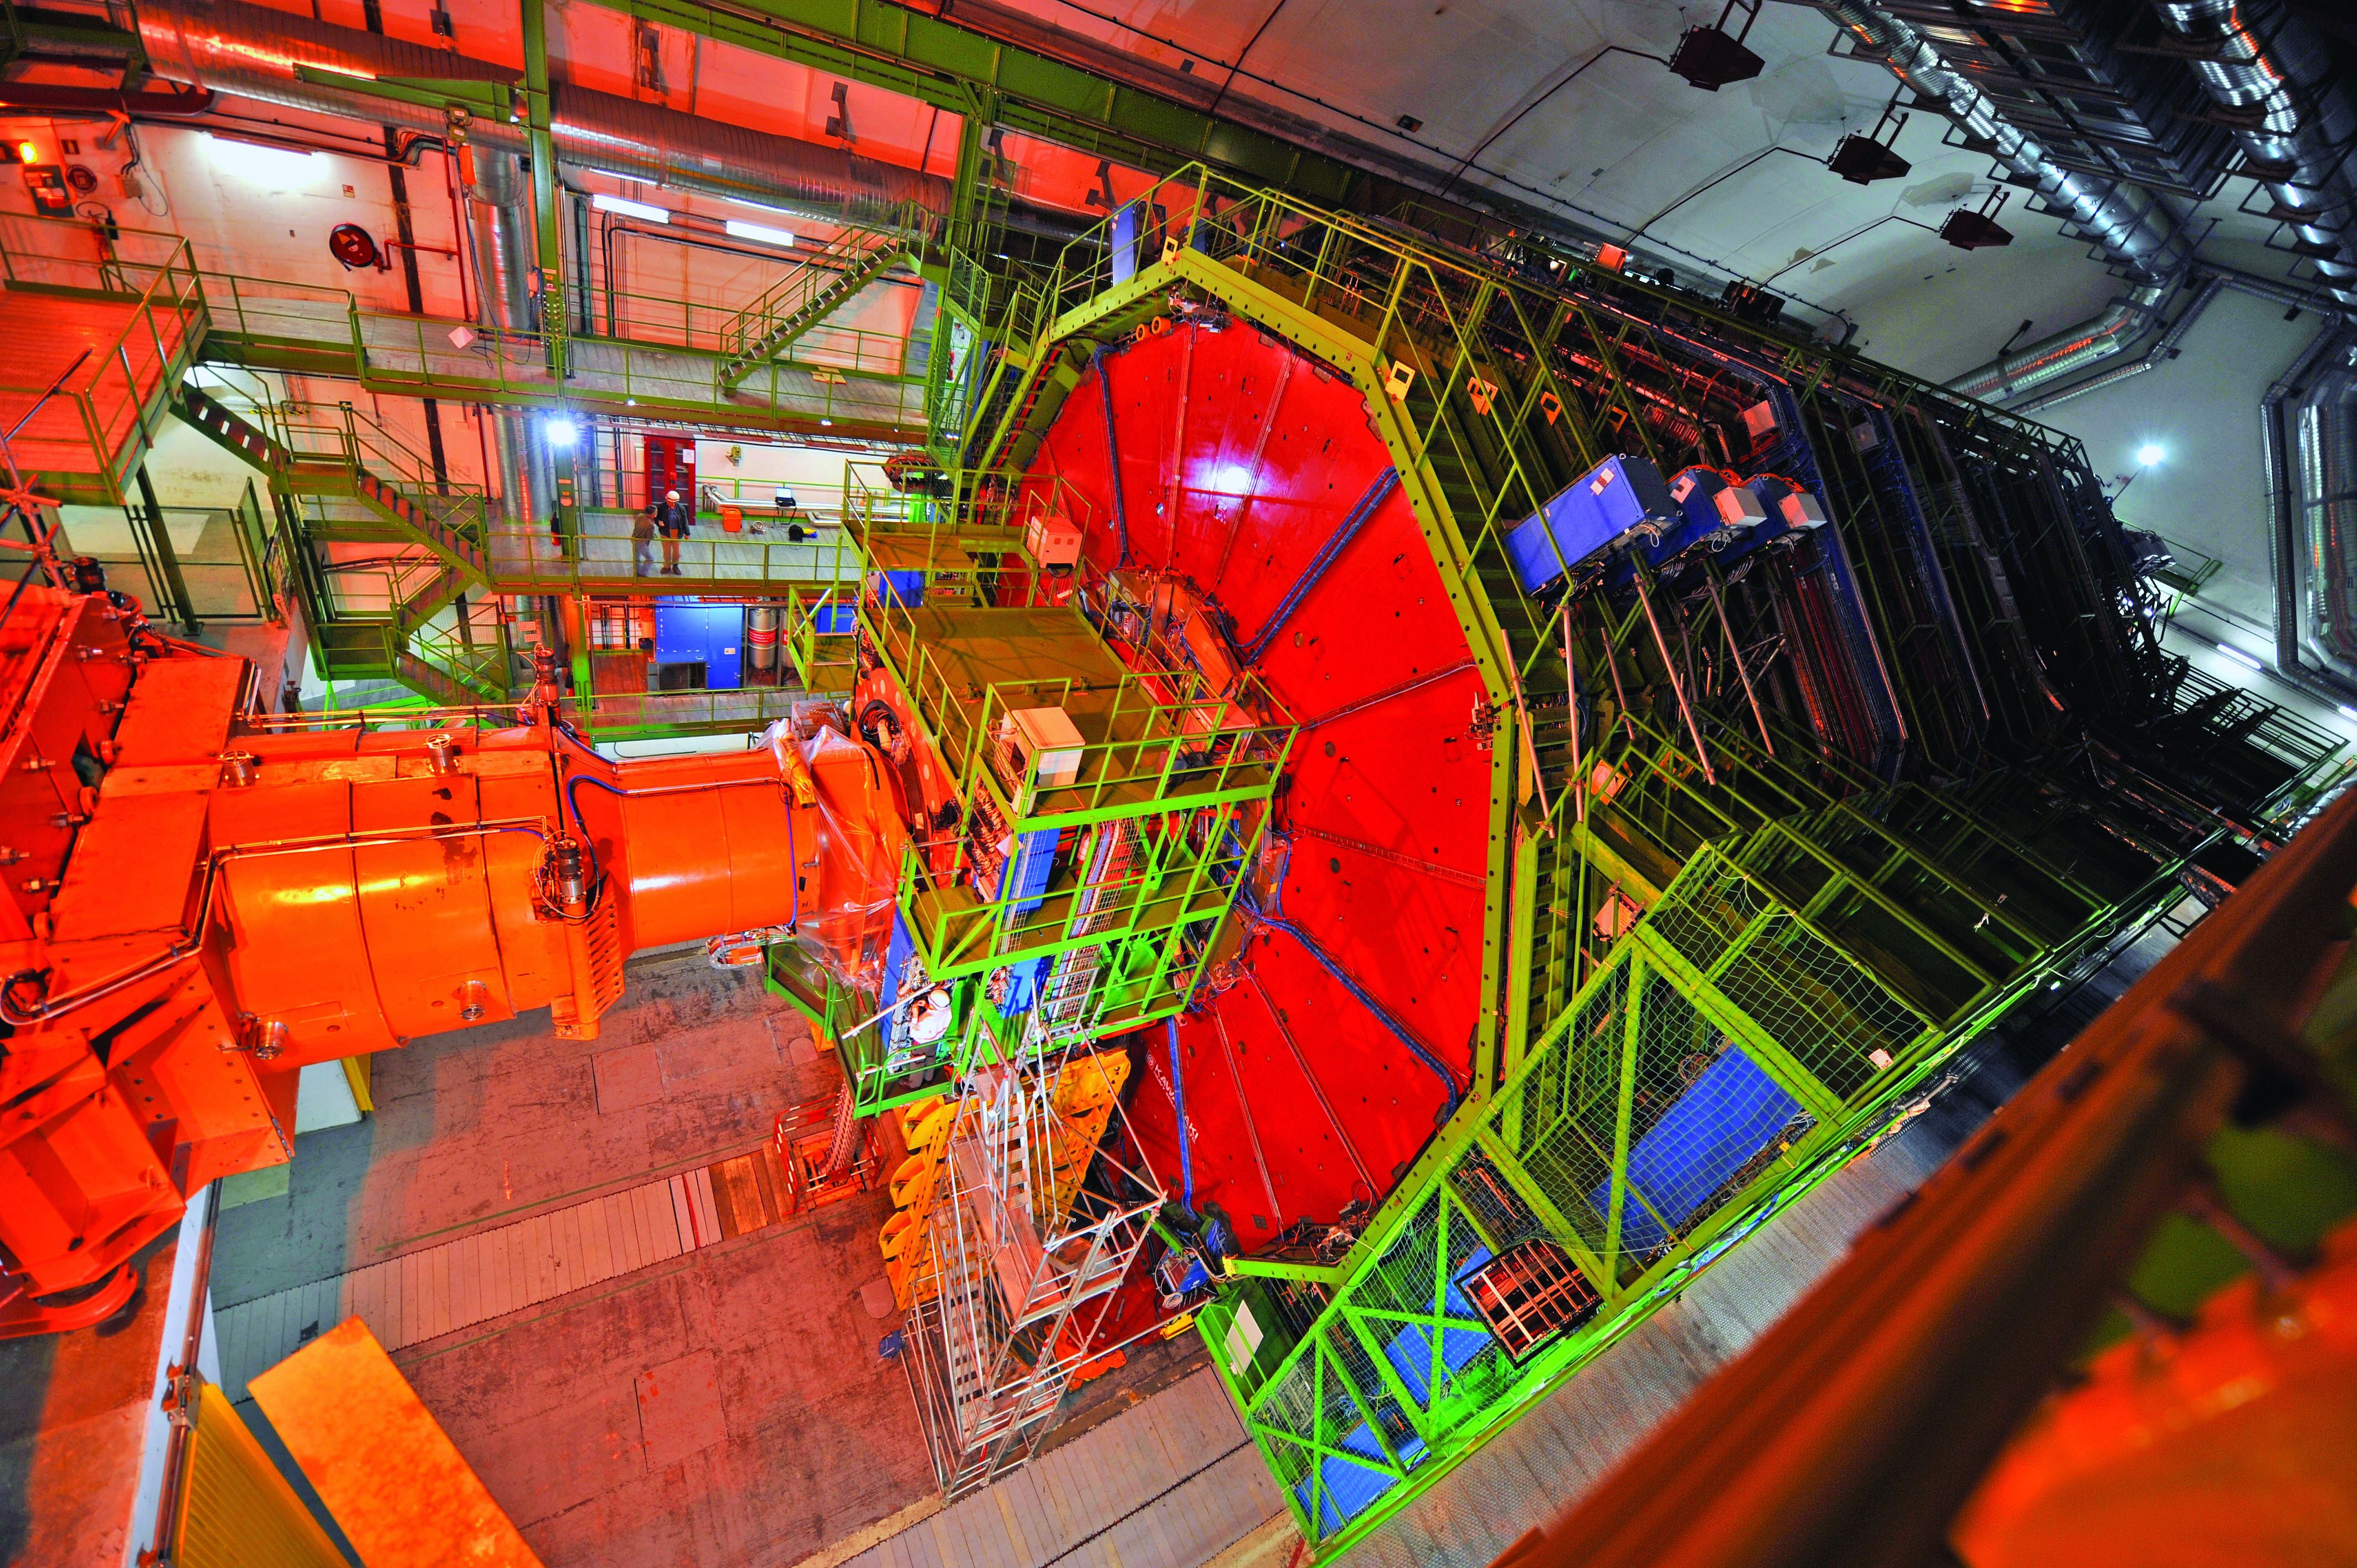
\includegraphics[width=0.492\textwidth,valign=c]{fig/cms/cms_picture3.jpg}}\quad
    \subfloat{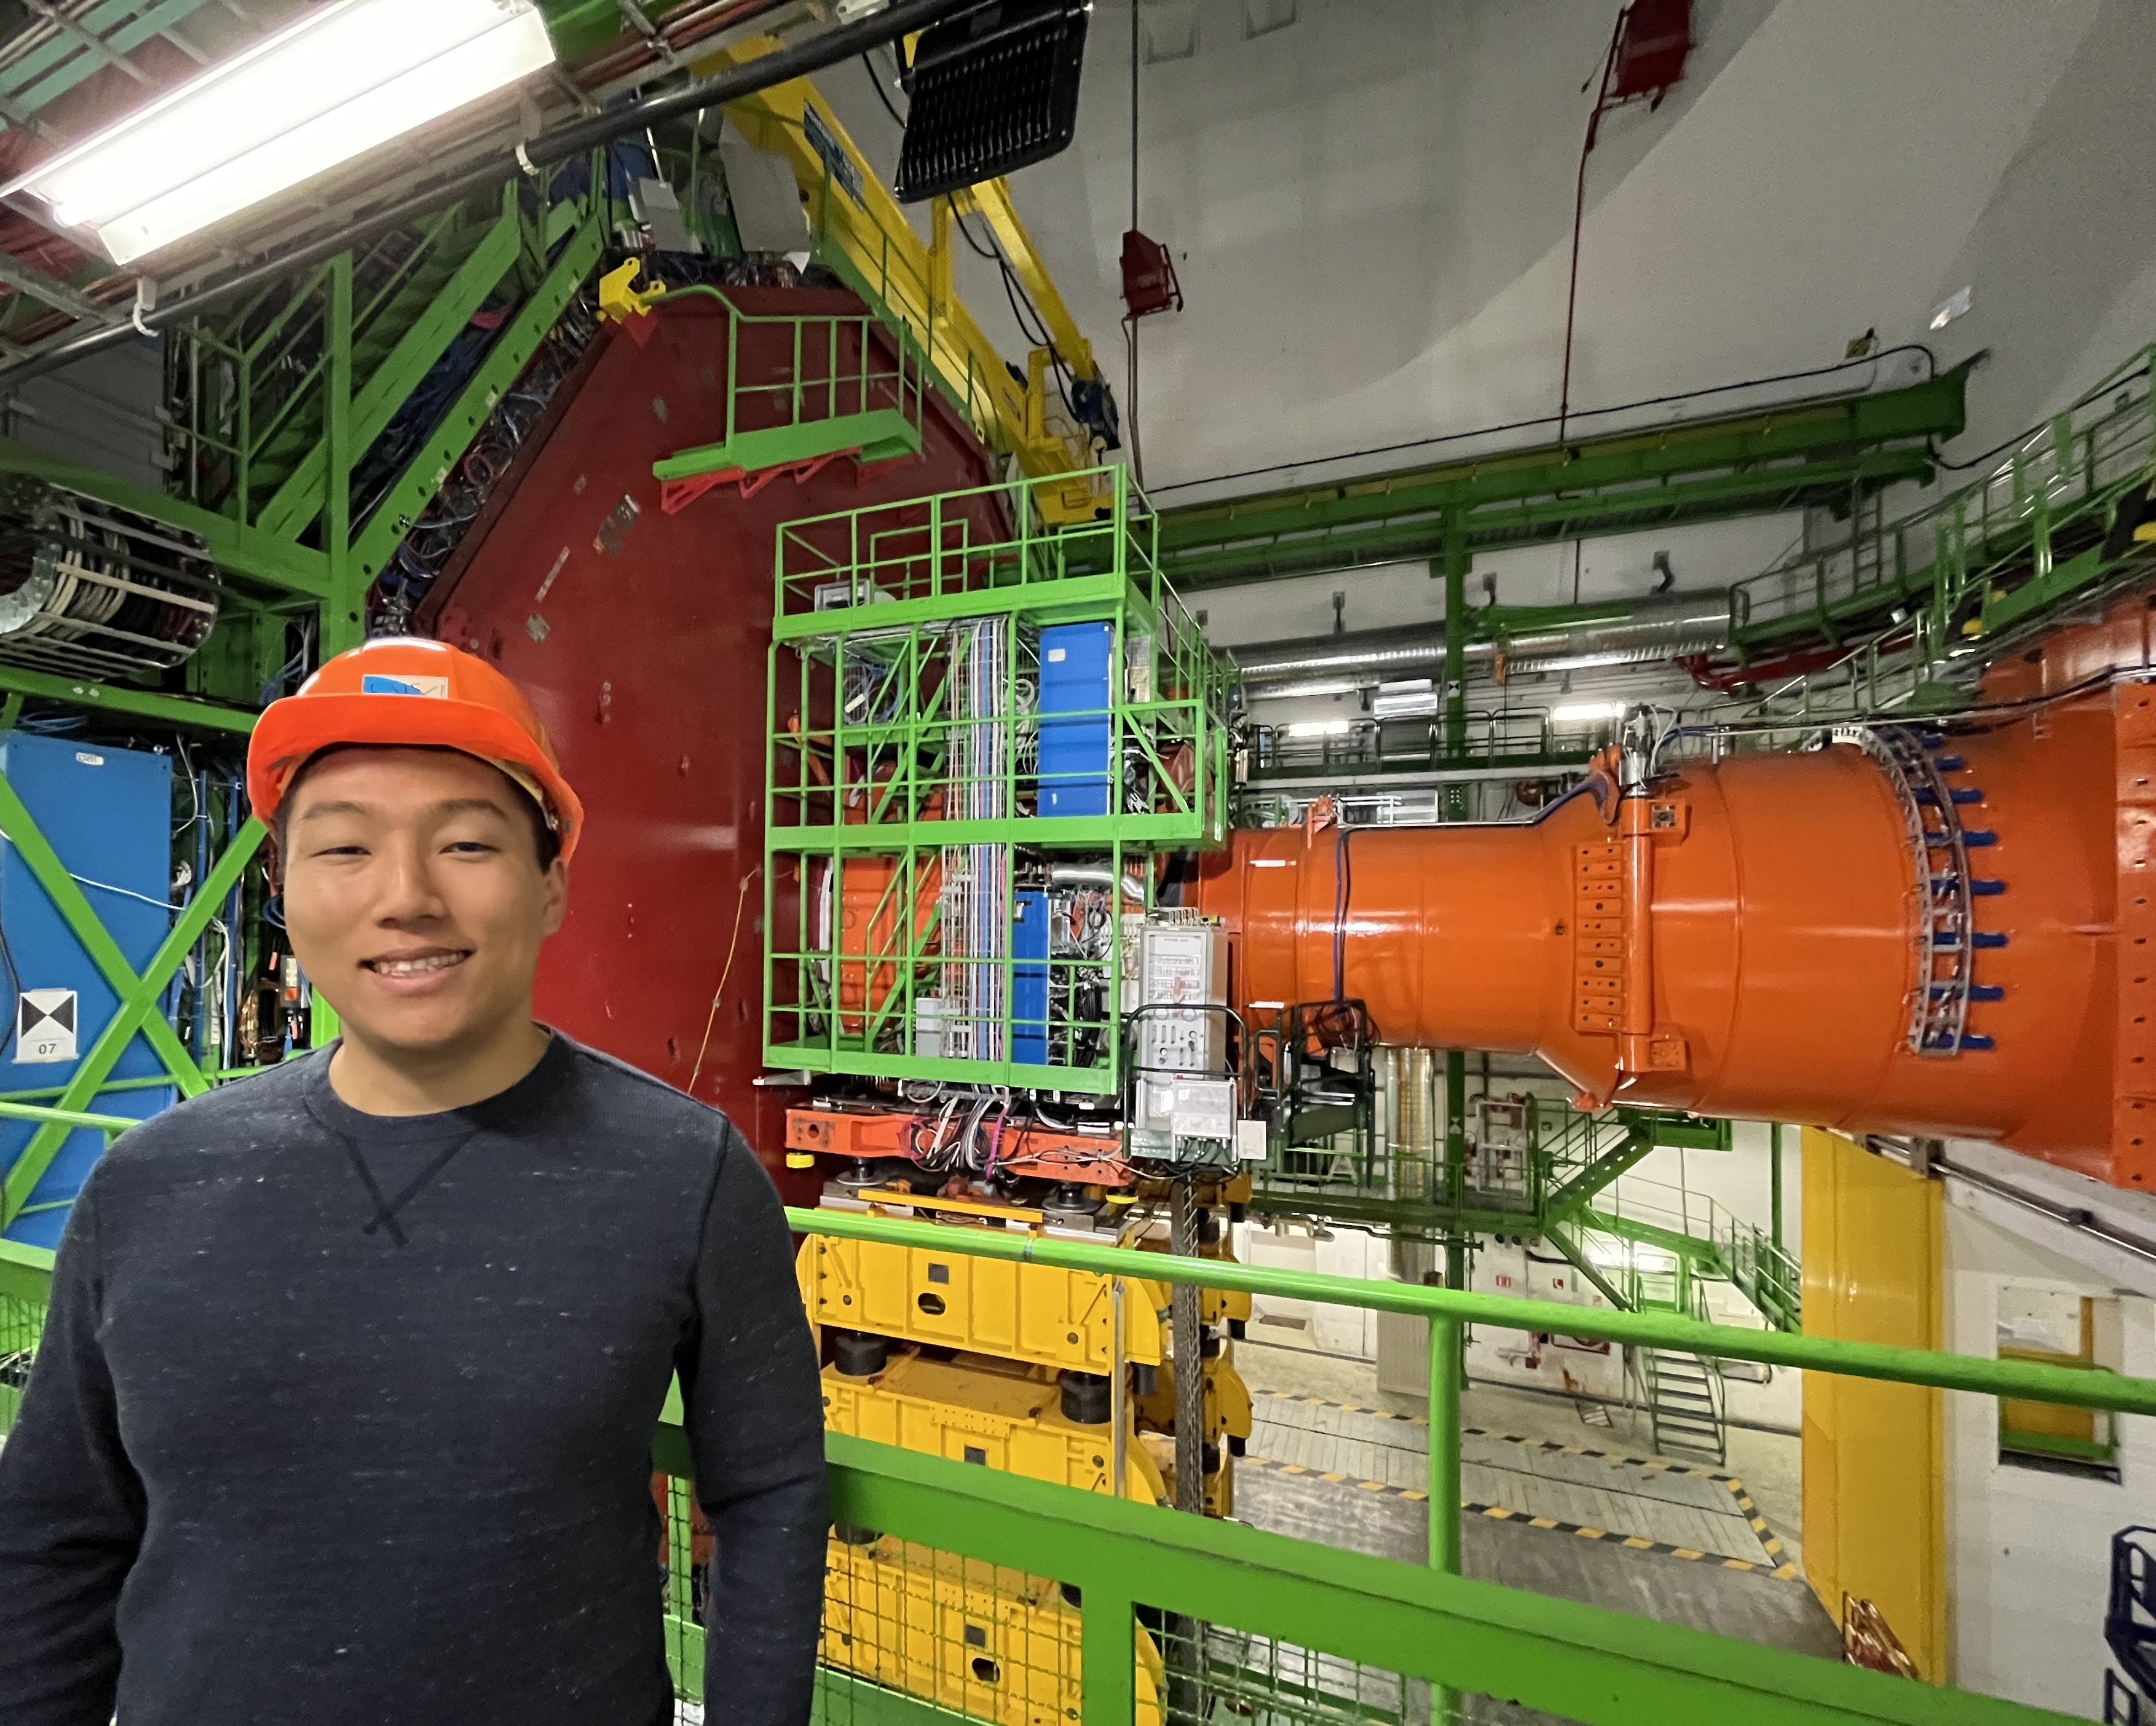
\includegraphics[width=0.408\textwidth,valign=c]{fig/cms/cms_jguiang.jpg}}
    \caption{
        The Compact Muon Solenoid in the closed configuration, pictured from the top (left) and side, with a physicist in the foreground for scale (right).
    }
    \label{fig:cms_jguiang}
\end{figure}

\subsection{Overview}
The CMS Experiment is composed of subdetectors arranged in layers, where each layer interacts with or completely absorbs certain particles, producing an electric signal that can be used to measure some property of those particles. 
The innermost layer is the silicon tracker, which allows for the reconstruction of the trajectories of throughgoing charged particles (``tracks''). 
Next is the electromagnetic calorimeter (ECAL), which absorbs electrons and photons and records their individual energies. 
After the ECAL, there is the hadronic calorimeter (HCAL), which instead absorbs hadrons and records their individual energies. 
These first three layers---the tracker, ECAL, and HCAL---are surrounded by the eponymous superconducting solenoid, which immerses them in an approximately uniform magnetic field that runs parallel to the beamline. 
This is critical: charged particles fly along curved trajectories in a magnetic field according to their charge and momentum, so those properties can be inferred from a high-quality measurement of each particle's trajectory. 
Finally, there are alternating layers of muon chambers, the other half of the experiment's namesake, and iron support structures. 
The former detects throughgoing muons, which pass through all of the inner layers mostly unperturbed, and measures an additional portion of their tracks.
However, the latter is equally important: the iron ``return yoke'' guides the magnetic field outside of the solenoid, absorbs stray particles that make it past the inner layers, and supports the immense weight of CMS itself. 
By combining information from all of these detectors, the exact identity of any individual particle can, in principle, be inferred based on which detectors registered a signal. 
Therefore, a full ``picture'' of each pp collision event is recorded by CMS for further study. 
The exact function of each subdetector layer described here is detailed below.

\subsection{Superconducting solenoid}
The curve of a track is critical, as it allows us to infer the charge and momentum of a particle. 
However, in a weak magnetic field, the particles produced at the LHC would have nearly straight tracks, due to the large pp collision energy. 
The magnetic field inside of CMS must therefore be very large~\cite{CMSWebMagnet}. 
It should also be nearly uniform everywhere in order to make the determination of each particle's charge and momentum as simple as possible. 
The CMS magnet must also be large in dimension, however, as it must surround the tracker, ECAL, and HCAL, since it would otherwise block outgoing particles. 

By winding copper wire into a helix and passing a current through it, we can generate an magnetic field whose strength is directly proportional to the current and number of turns of the wire, but inversely proportional to the length of the helix. 
Within the volume of the helix, the magnetic field will be almost uniformly oriented in a single direction, determined by the orientation of the helix and direction of the current (Fig.~\ref{fig:cms_magnet_ideal}). 
This is not true outside of the helix where the magnetic field lines curve in space. 

\begin{figure}[htb]
    \centering
    \subfloat[]{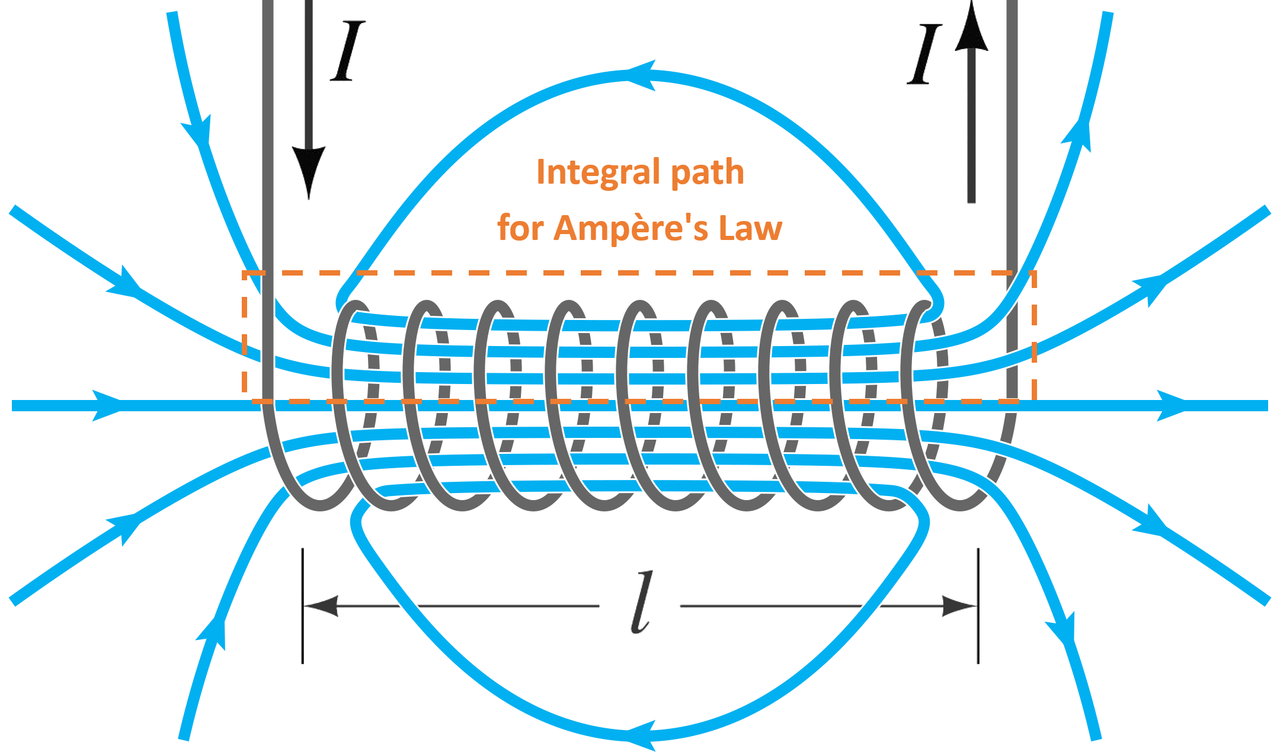
\includegraphics[width=0.4\textwidth,valign=c]{fig/cms/solenoid_ideal.png}\label{fig:cms_magnet_ideal}}\quad
    \subfloat[]{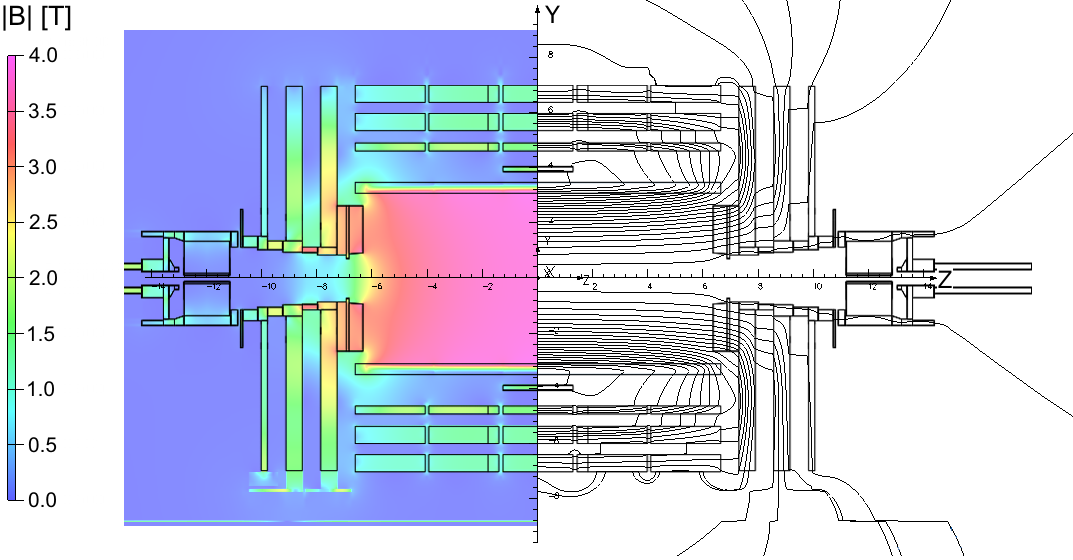
\includegraphics[width=0.5\textwidth,valign=c]{fig/cms/solenoid_field.png}\label{fig:cms_magnet_field}}
    \caption{
        The field lines of an ideal solenoid (a) and those of the CMS magnet (b), from Ref.~\cite{CMS:2009moq}. 
        For the ideal solenoid, the magnetic field is described by a simple equation: $B = \mu_0\frac{NI}{l}$, where $\mu_0$ is the magnetic constant, $N$ is the number of turns, $I$ is the current, and $l$ is the length of the helix. 
    }
    \label{fig:cms_fields}
\end{figure}

The CMS magnet~\cite{CERN-LHCC-97-010} is a massive\footnotemark{} realization of a solenoid. 
\footnotetext{It was built offsite, however, so it needed to be designed to fit within 7 such that it could be wheeled through the streets in Cessy, France (under which CMS is situated)~\cite{CMSWebMagnet}.}
It is comprised of over 2000 turns of Rutherford wire, which has a rectangular cross section (Fig.~\ref{fig:cms_magnet}). 
In operation, it is cooled to superconducting temperatures (-268.5 \de{}C, or one degree warmer than outer space), such that a high current of 20 kiloamperes\footnotemark{} can be passed through the coil without destroying it. 
\footnotetext{For scale, this is 100\,000 times larger than the minimum fatal current for humans (100--200 milliamperes)~\cite{10.1093/ptj/46.9.968}.}
This configuration allows the CMS magnet to produce a mostly uniform magnetic field of 4 T inside of the solenoid volume. 
That is 2--4 times larger than an MRI, which are typically 0.5--1.5 T~\cite{Berger2002-gs}, within a volume that is 1000 times larger. % TODO: citation needed for volume of an MRI?
We must also, however, have a fairly uniform magnetic field outside of the solenoid in order to maintain good momentum resolution for muons. 
To achieve this, the iron support structures that hold CMS together are also designed to guide the magnetic field lines (Fig.~\ref{fig:cms_magnet_field}). 
Inside of the iron, the magnetic field runs almost uniformly parallel to the field inside of the solenoid, but in the opposite direction---this gives muon tracks a characteristic S-shape in the transverse plane. 

\begin{figure}[htb]
    \centering
    \subfloat{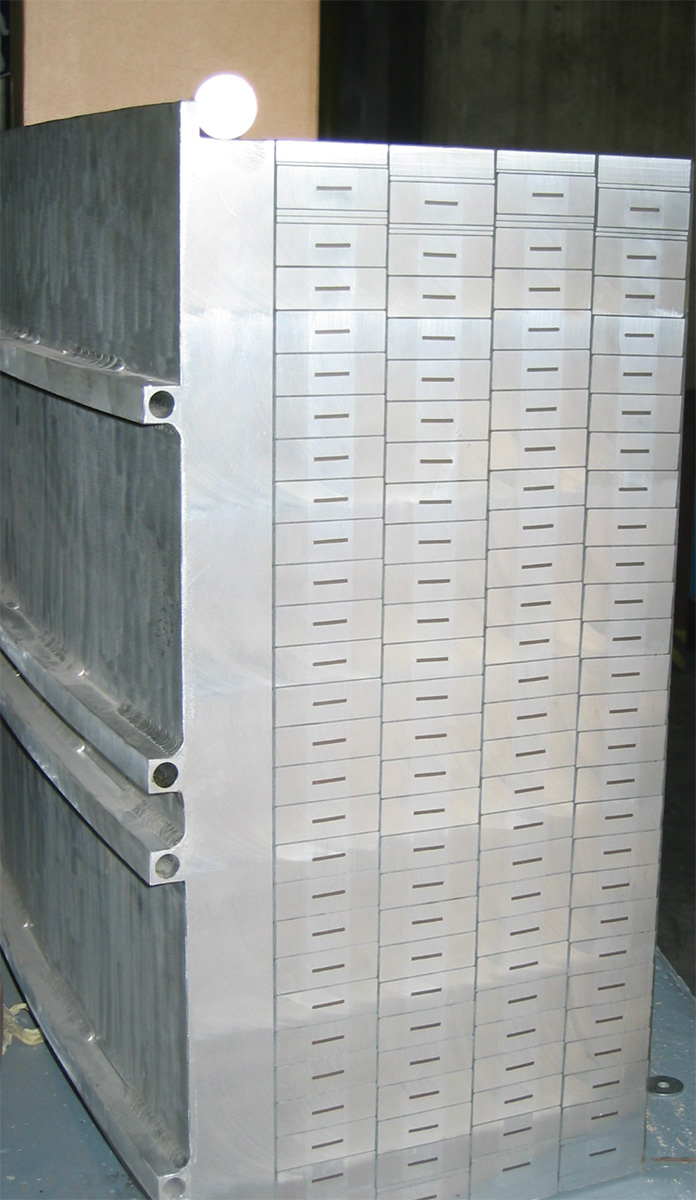
\includegraphics[width=0.3\textwidth,valign=c]{fig/cms/solenoid_wedge.jpg}}\quad
    \subfloat{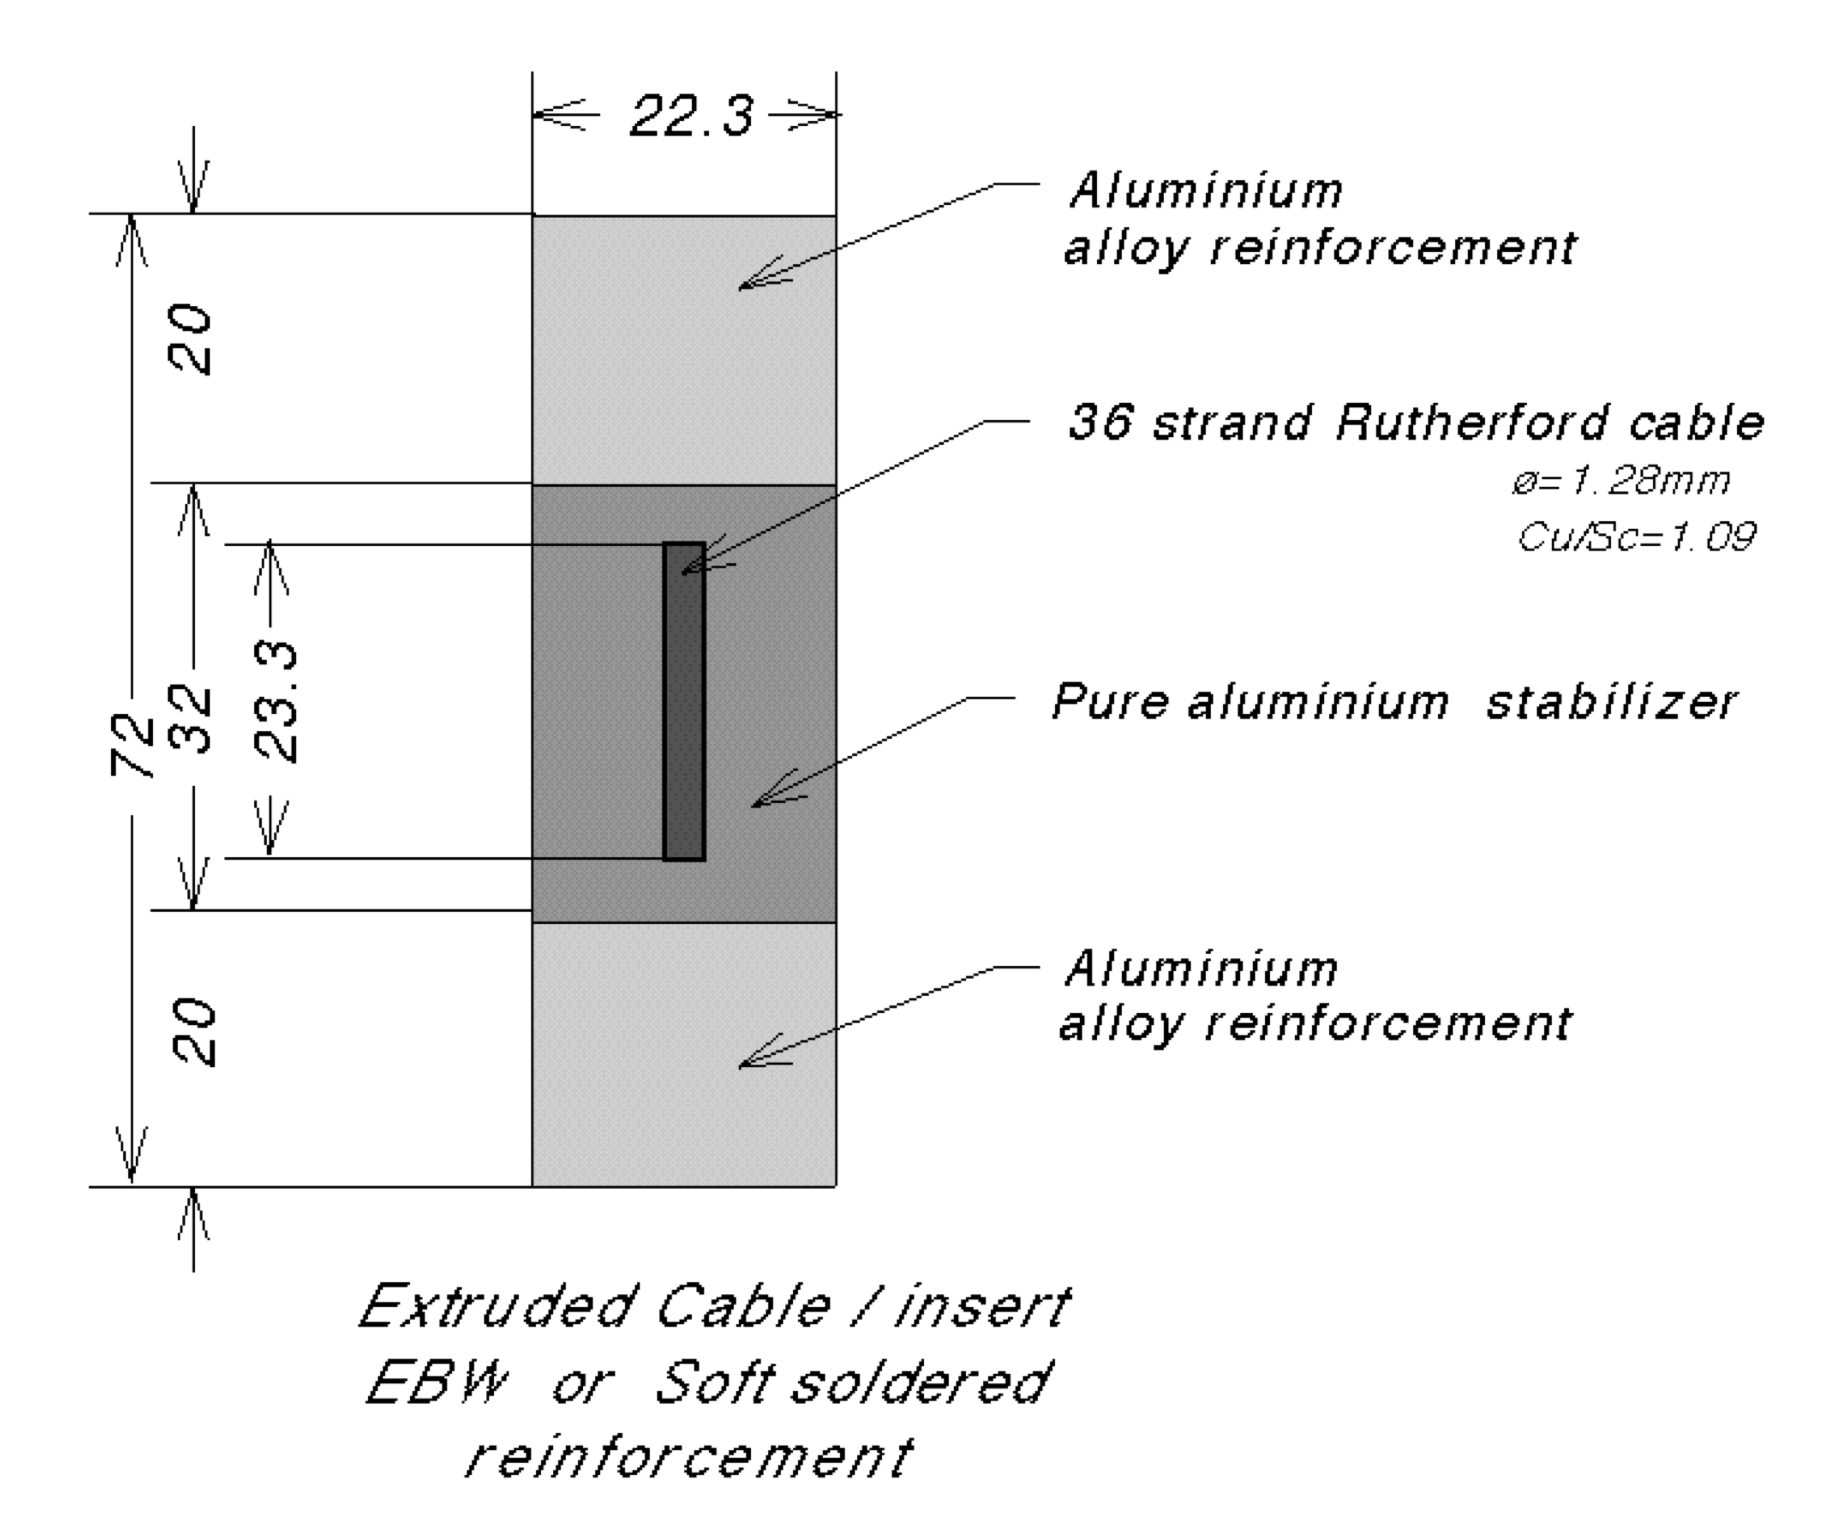
\includegraphics[width=0.6\textwidth,valign=c]{fig/cms/solenoid_cable.png}}
    \caption{
        A photograph of a section of the CMS magnet, from Ref.~\cite{CourierSolenoid}, showing the cross section of the solenoid windings (left), and a diagram of a single winding, from Ref.~\cite{CERN-LHCC-97-010} (right). 
    }
    \label{fig:cms_magnet}
\end{figure}

\subsection{Silicon tracker}
In order to reconstruct the track of any particle, we need its position at multiple points in time. 
A tracker records these positions. 
Mechanically, this can be done in a variety of ways. 
Some of the earliest particle physics experiments used bubble chambers, a device that maintains (for a brief instance) a volume of superheated liquid immersed in a magnetic field in which throughgoing charged particles leave helical trails of bubbles. 
Photographs of these trails were used to infer the identities of each particle. 
Still others used even more exotic non-electric solutions, like the OPERA Experiment, which used enormous layers of nuclear emulsion film (modified photography film) in which throughgoing particles would leave tiny black dots after the film was developed\footnotemark{}~\cite{Acquafredda:2009zz}---the experiment used over 100\,000 m$^2$ of emulsion film in total. 
\footnotetext{Developing the film was quite an operation, and a large robotic arm was used to remove and replace the layers.}

The leading challenge in designing the CMS tracker was the unprecedented level of radiation, due to the high frequency of pp collisions which each produce many thousands of particles. 
Existing tracker designs, like the CDF Experiment's beautiful gas-and-wire tracker~\cite{CDF:2003xbh}, would quickly break down\footnotemark{} in this kind of environment.
\footnotetext{In fact, the tracker section was left blank in the first CMS design document, since there were no known solutions at the time~\cite{CMSWebTracker}.}
Thankfully, advances in radiation-hard electronics yielded a new solution. 
In particular, a silicon-based tracking module was devised. 
When charged particles pass through the module, they liberate electrons from the silicon atoms. 
These electrons are collected one of several small readout plates, which results in a localized electric signal called a ``hit,'' giving excellent spatial resolution. 

The CMS tracker is composed of multiple layers of silicon tracker modules (Fig.~\ref{fig:cms_tracker_layout}), such that each throughgoing particle leaves multiple hits that can then be used to reconstruct its track. 
The layers are grouped into different sections according to their proximity to the beamline and their geometry. 
The innermost layers comprise the ``inner tracker'' (Fig.~\ref{fig:cms_tracker_inner}). 
In these layers, pixel modules are used because they have superior spatial resolution, allowing us to measure the first portion of each track precisely. 
The outermost layers comprise the ``outer tracker'' (Fig.~\ref{fig:cms_tracker_outer}). 
These layers use strip modules, which have worse spatial resolution than the pixel modules, but are easier to produce. 

\begin{figure}[htb]
    \centering
    \subfloat[]{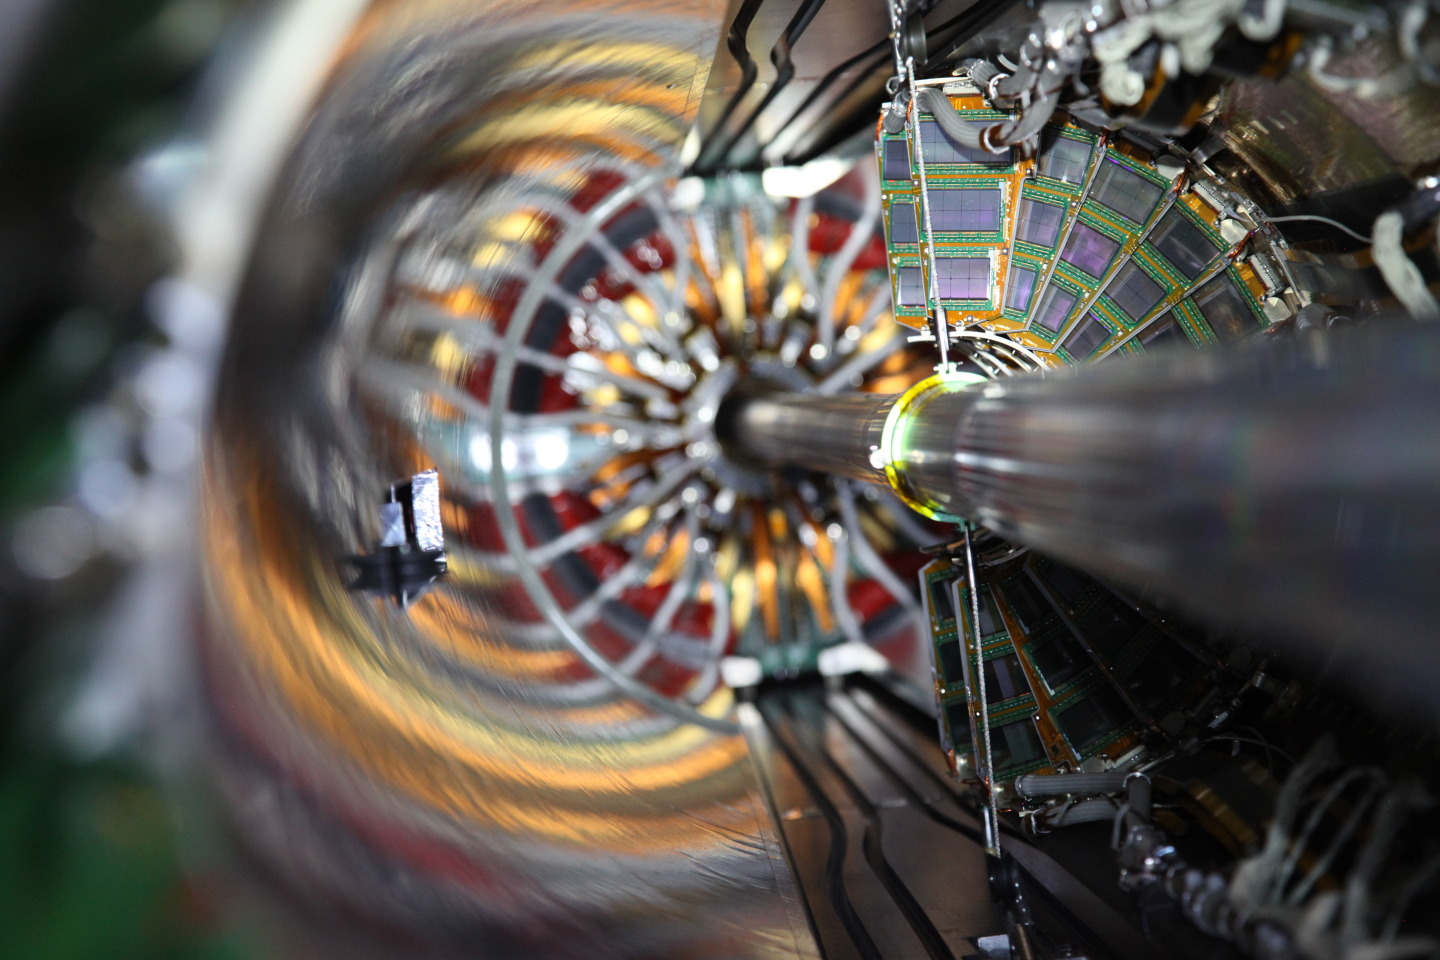
\includegraphics[width=0.45\textwidth,valign=c]{fig/cms/tracker_pixels.jpg}\label{fig:cms_tracker_inner}}\quad
    \subfloat[]{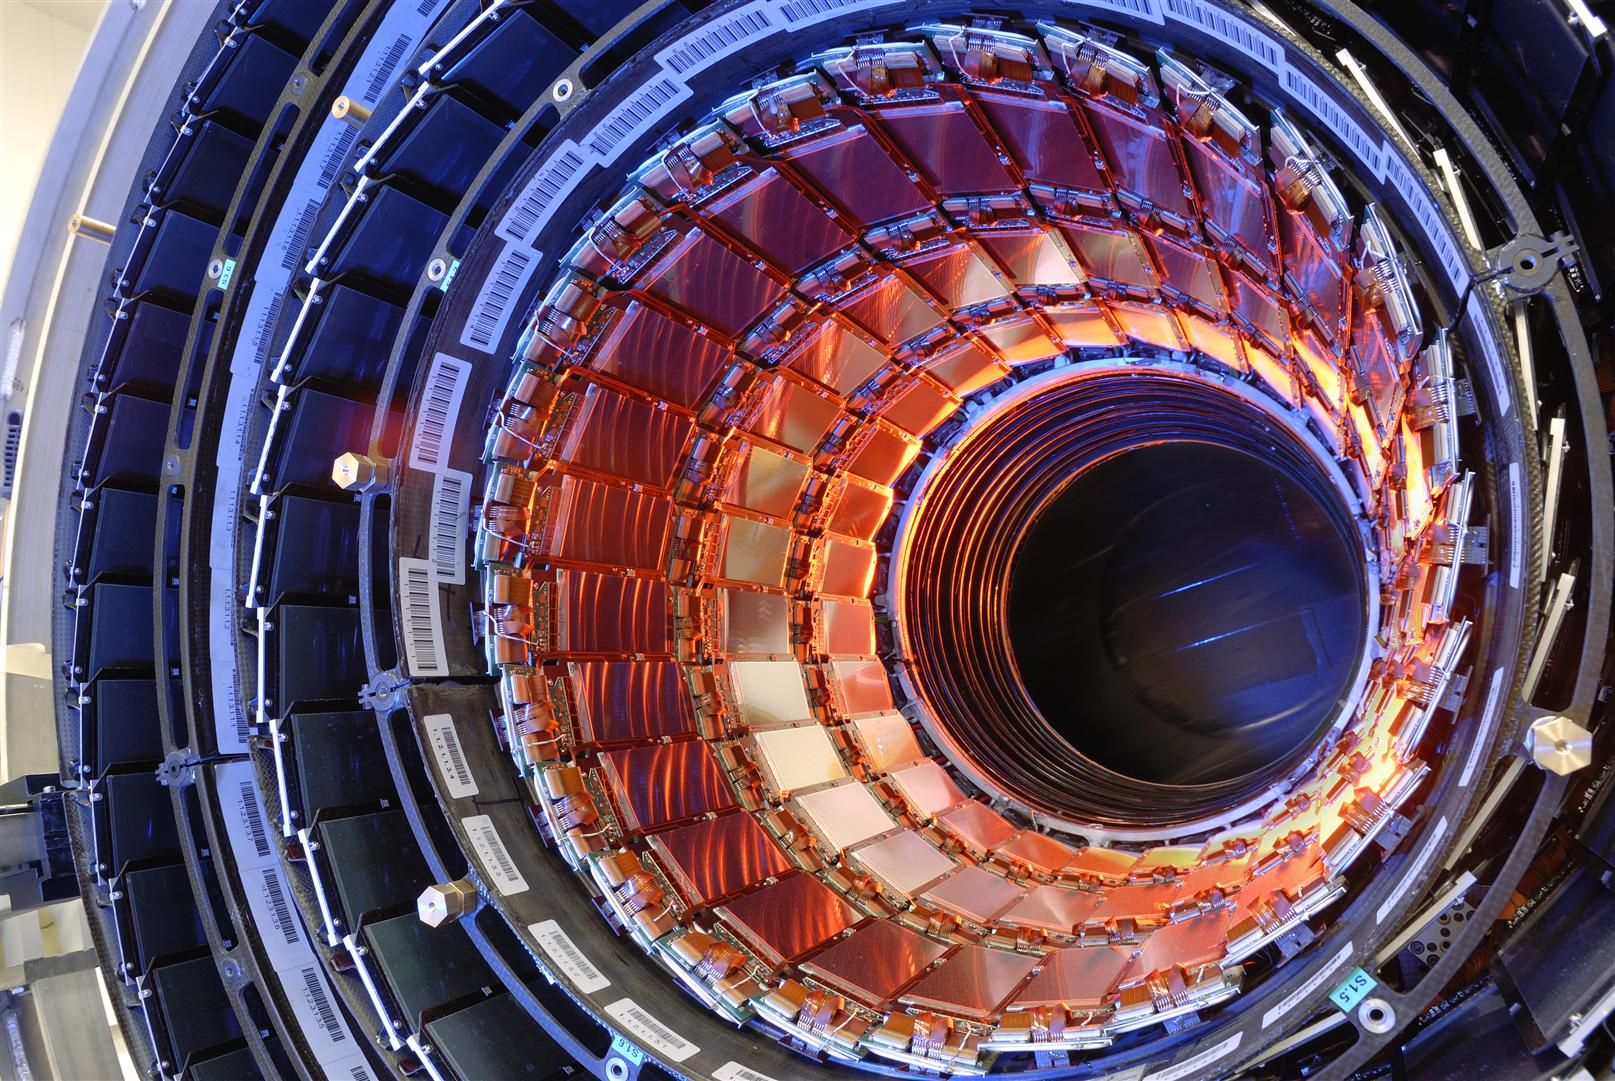
\includegraphics[width=0.45\textwidth,valign=c]{fig/cms/tracker_rainbow.jpg}\label{fig:cms_tracker_outer}}
    \caption{
        A photograph of the inner forward pixel modules (left), from Ref.~\cite{Hoch:2017264}, and the outer barrel layers with a physicist for scale (right), from Ref.~\cite{Maximilien:995912}, of the CMS tracker. 
    }
    \label{fig:cms_tracker_pictures}
\end{figure}

\begin{figure}[htb]
    \centering
    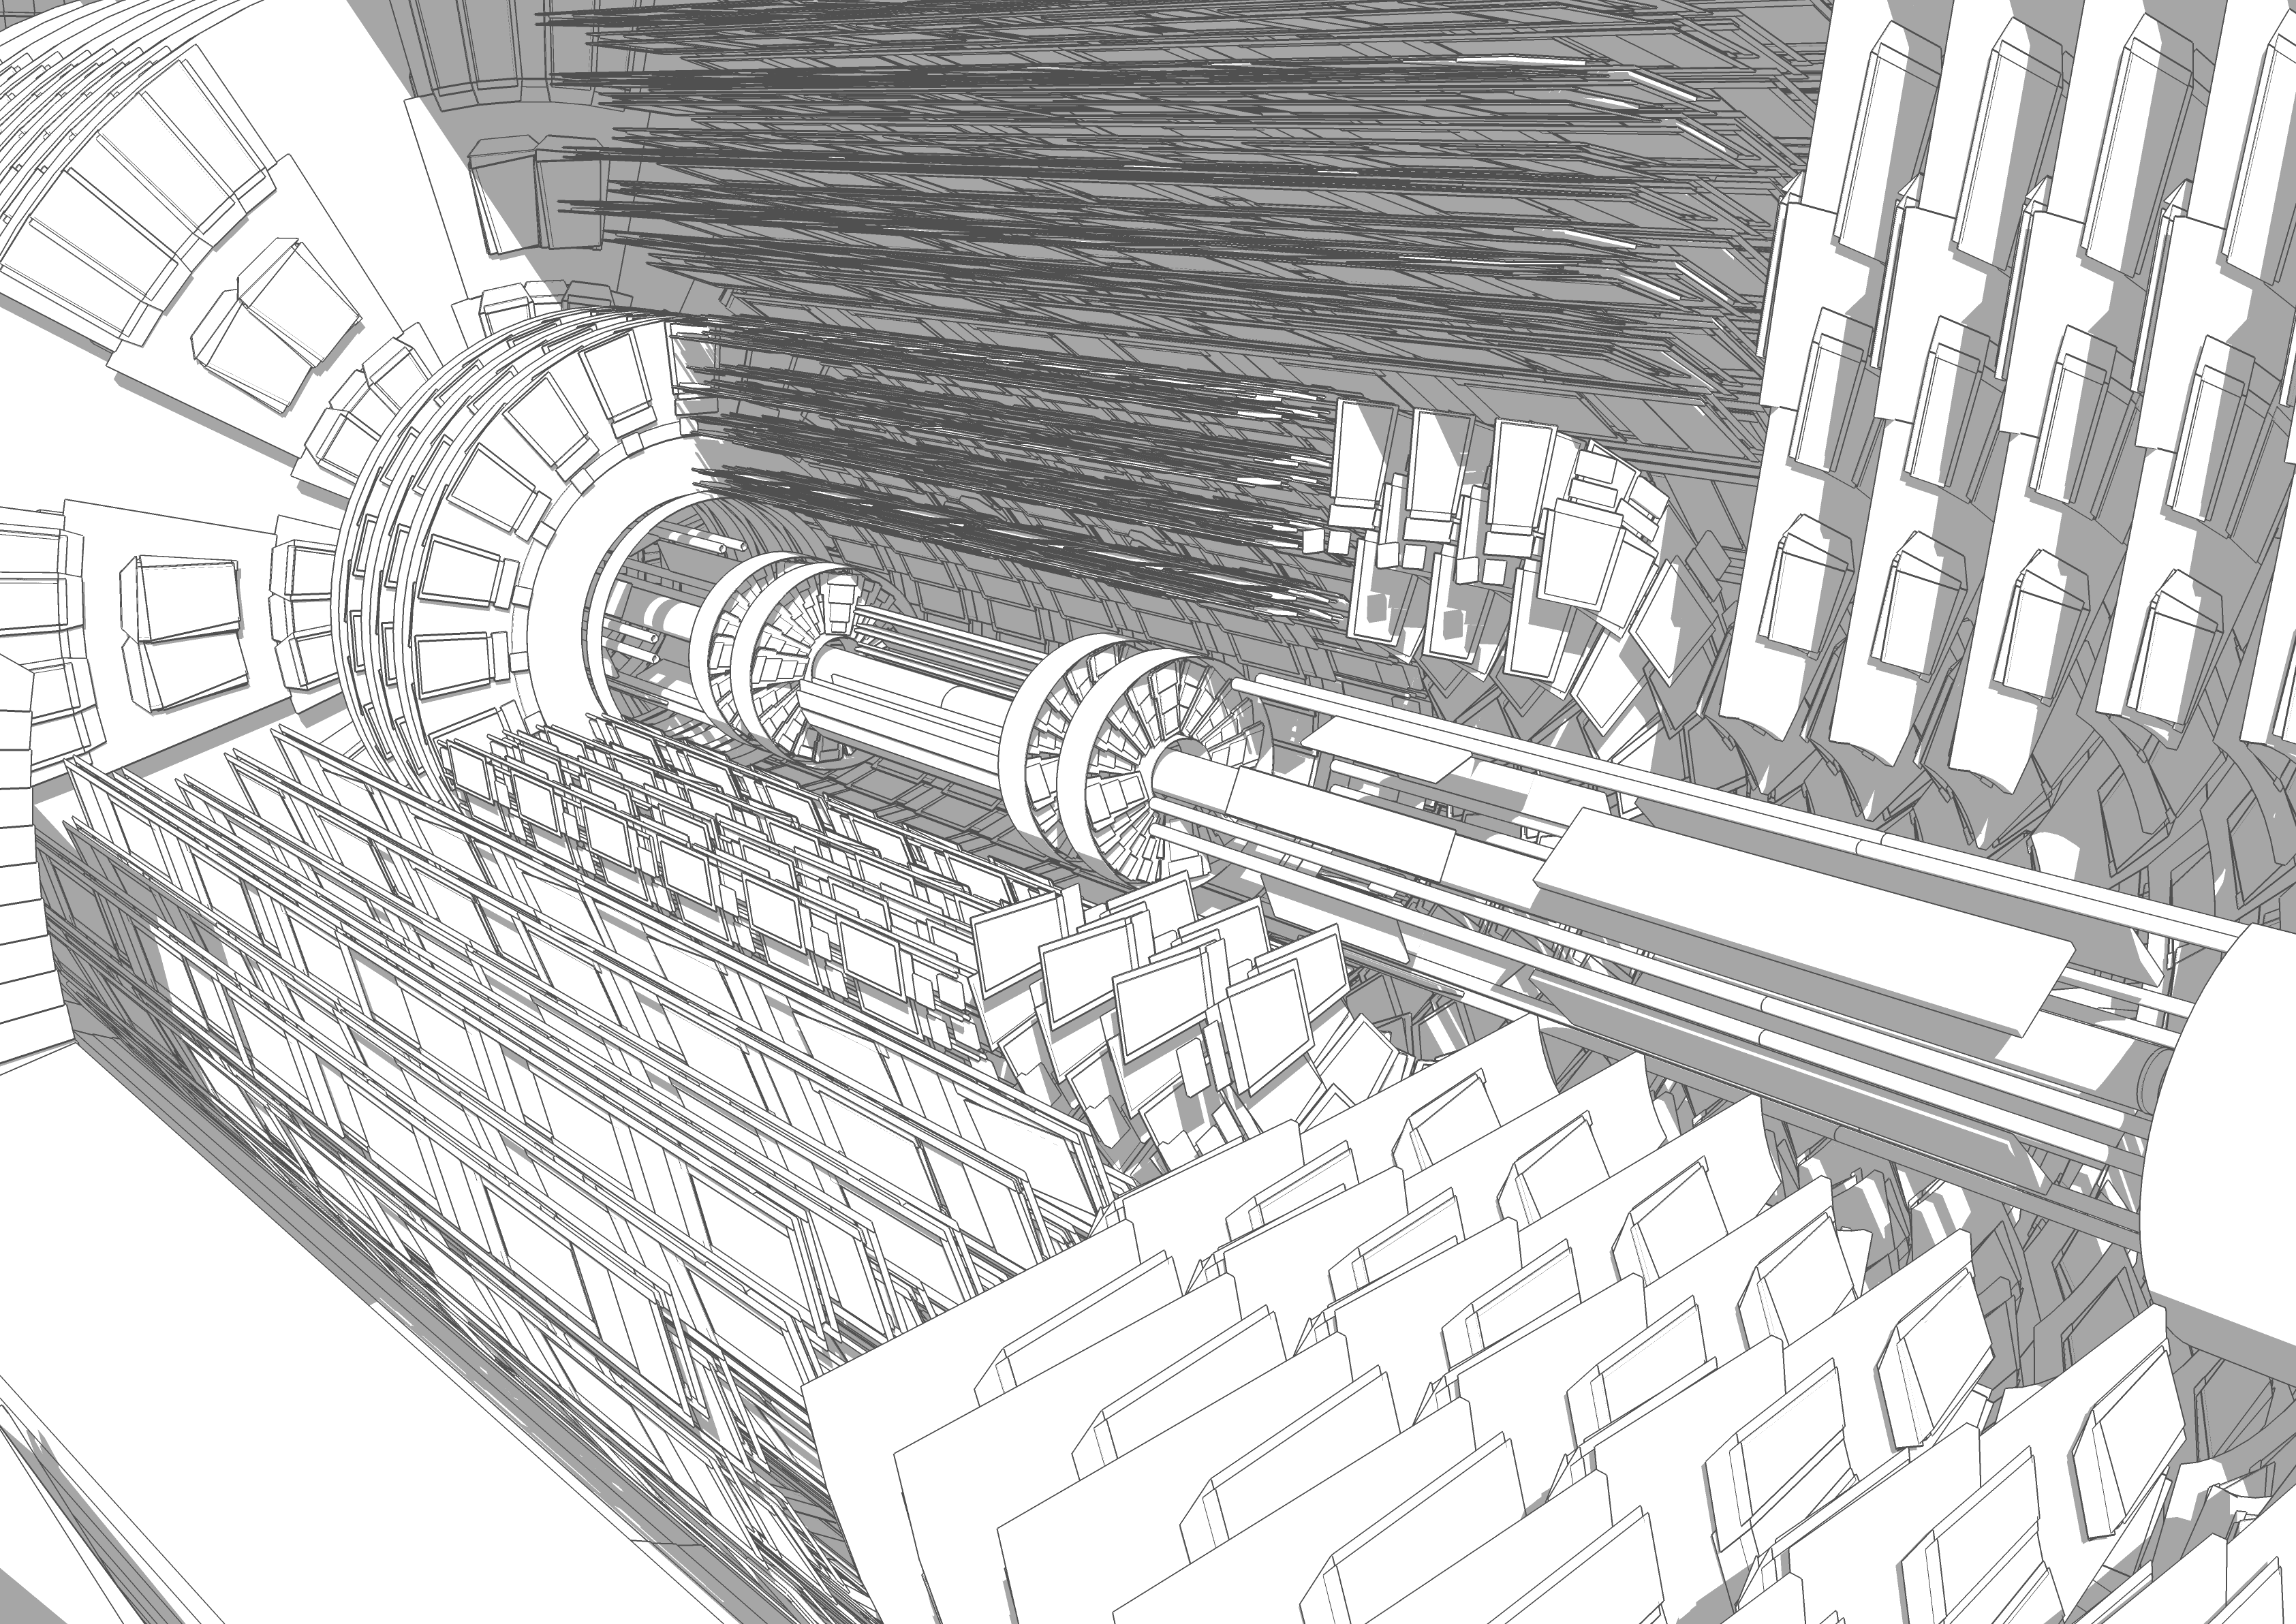
\includegraphics[width=0.9\textwidth,valign=c]{fig/cms/tracker_detailed.png}
    \caption{
        A detailed cutaway diagram of the CMS Phase-1 tracker, from Ref.~\cite{Sakuma:2630160}. 
    }
    \label{fig:cms_tracker_layout}
\end{figure}

\subsection{Electromagnetic calorimeter}
The ECAL (Fig.~\ref{fig:cms_ecal_install}) consists of nearly 80\,000 lead tungstate (PbWO$_4$) crystals\footnotemark{} (Fig.~\ref{fig:cms_ecal_crystal})~\cite{CMSWebECAL}. 
\footnotetext{These crystals were grown in manufacturing plants in Russia and China and took roughly a decade to produce~\cite{CMSWebECAL}.}
When an electron or photon passes through one of these crystals, they interact through the electromagnetic force with the atoms in the crystal lattice, producing a shower of photons. 
This process is called ``scintillation'' and the amount of light produced from one of these interactions is proportional to the energy of the impinging particle. 
Each PbWO$_4$ crystal is glued to a photodetector that collects the scintillation light by the attached crystal and outputs an electric signal proportional to the amount of light collected. 
This signal can then be used to measure the energy of electrons and photons. 

The probability of material interactions ocurring as well as the shape of the shower varies amongst scintillating materials. 
Ultimately, PbWO$_4$ was selected for its short radiation length and small Moli\`ere radius~\cite{CERN-LHCC-97-033}, corresponding to a high probability of interactions and showers localized mostly to a single crystal, respectively. 
The former property is most obviously useful: a high probability of scintillation means electrons and photons are more efficiently collected by the ECAL. 
The latter property, however, is also vital: localized showers are less likely to overlap, so individual particles can be resolved. 

\begin{figure}[htb]
    \centering
    \subfloat[]{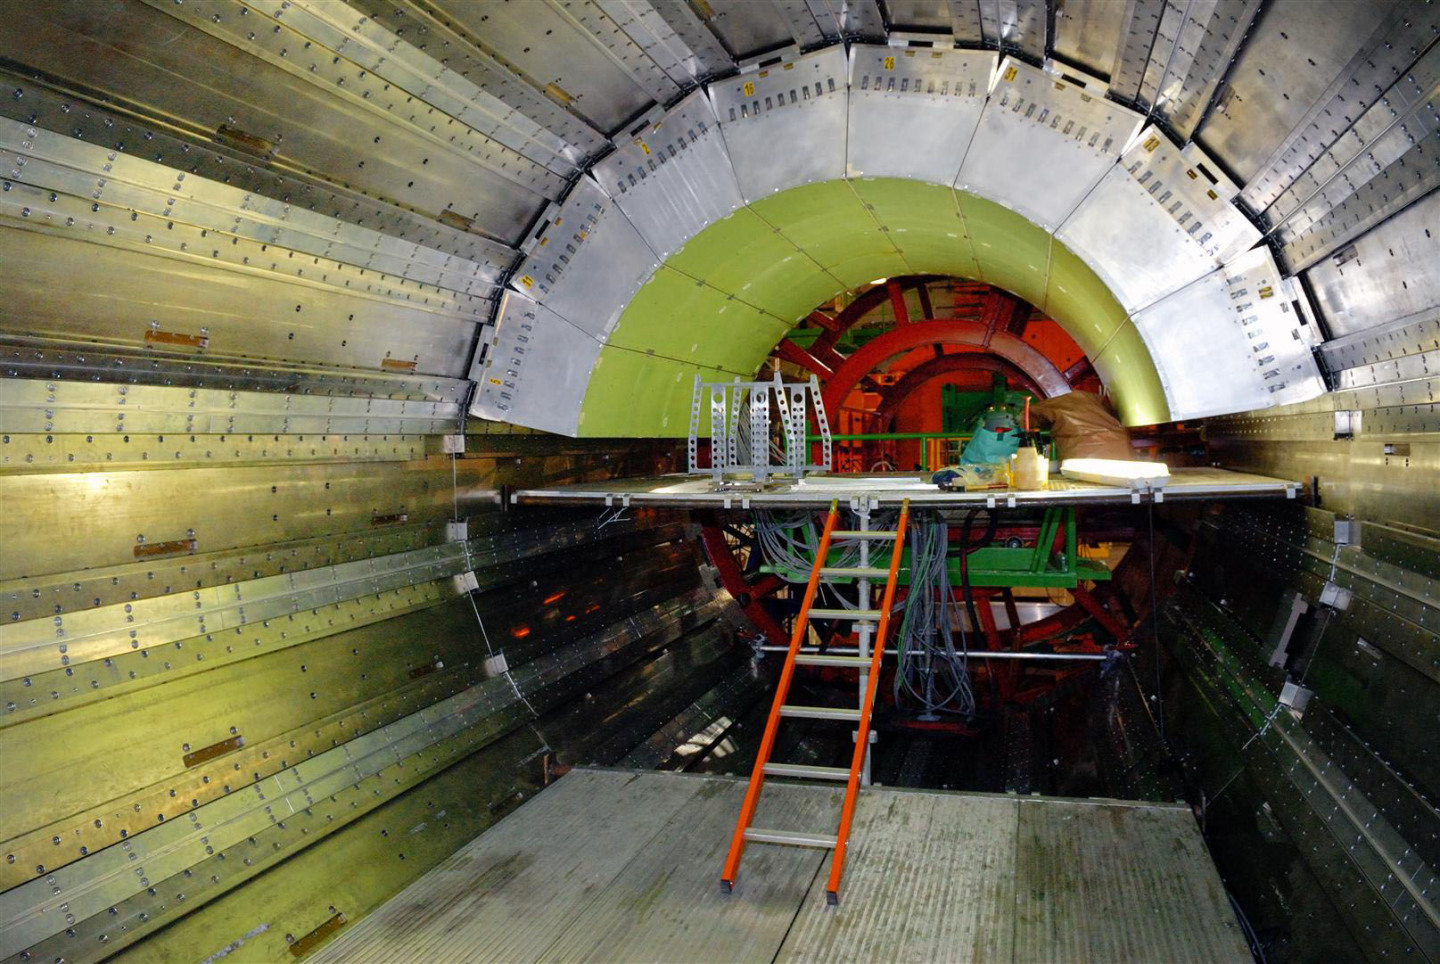
\includegraphics[width=0.45\textwidth,valign=c]{fig/cms/ecal_install.jpg}\label{fig:cms_ecal_install}}\quad
    \subfloat[]{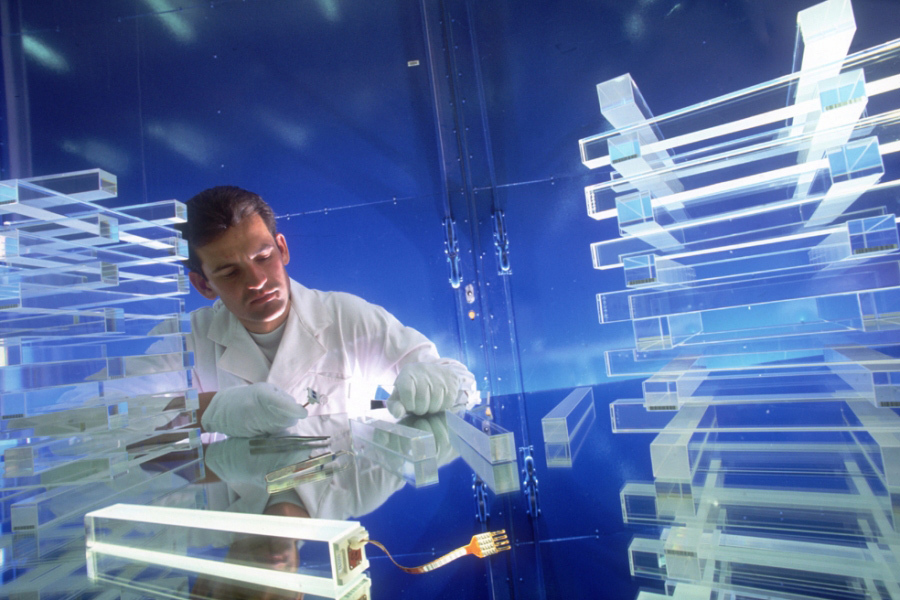
\includegraphics[width=0.45\textwidth,valign=c]{fig/cms/ecal_crystal.jpg}\label{fig:cms_ecal_crystal}}
    \caption{
        A photograph of the CMS electromagnetic calorimeter (ECAL) after half of the modules had been installed (left) and a physicist posed with the lead tungstade scintillator crystals used in the ECAL (right). 
        Both photographs are from Ref.~\cite{Brice:1431477}.
    }
    \label{fig:cms_ecal}
\end{figure}

\subsection{Hadronic calorimeter}
The HCAL (Fig.~\ref{fig:cms_hcal_removed}) is composed of interwoven layers of solid brass or steel plates and plastic scintillator tiles~\cite{CERN-LHCC-97-031}. 
When a hadron interacts with one of the brass and steel ``absorber'' layers, a shower of secondary particles are created. % TODO: add some sort of shower pic, there is one in Kolanoski & Wermes (particle detectors book)
The secondary particles pass through the next scintillator layer, creating scintillation light, then proceed to the next absober layer. 
In this way, large cascading showers of secondary particles are produced according to the energy of the impinging particle, where each scintillator layer gives some measurement, or ``sample,'' of the original particle's energy. 

This kind of calorimeter, which has alternating absorber and scintillator layers, is called a ``sampling'' calorimeter as opposed to a ``homogenous'' calorimeter, wherein a single medium is used to both create the shower and measure the energy. 
Sampling calorimeters are typically less costly and give some information on the shape of the shower, whereas homogenous calorimeters have superior energy resolution. 
In addition, almost all hadronic calorimeters are sampling calorimeters, homogenous hadronic calorimeter would need to be infeasibly large in order to contain a hadronic shower~\cite{KolanoskiWermesDetectors}. 
It is even more critical that the HCAL be compact for CMS, as every increase in size of the inner layers results in large increases in volume of the solenoid and muon chambers, resulting in enormous increases in energy and material costs. 
Due to these space constraints, an additional layer of the HCAL needed to be placed outside of the magnet in order to measure, and absorb, anything that made it past the bulk of the HCAL. 
In fact, the HCAL was already projected to be too costly due to the sheer amount of high-quality brass needed to create the absorber plates. 
To save on costs, the Russian Navy was convinced---without much difficulty---to recycle over one million World War II artillery shells (Fig.~\ref{fig:cms_hcal_russian}), which were designed to withstand large amount of stress (read: explosions) and years at sea, for the cause~\cite{CMSWebHCAL}. 

\begin{figure}[htb]
    \centering
    \subfloat{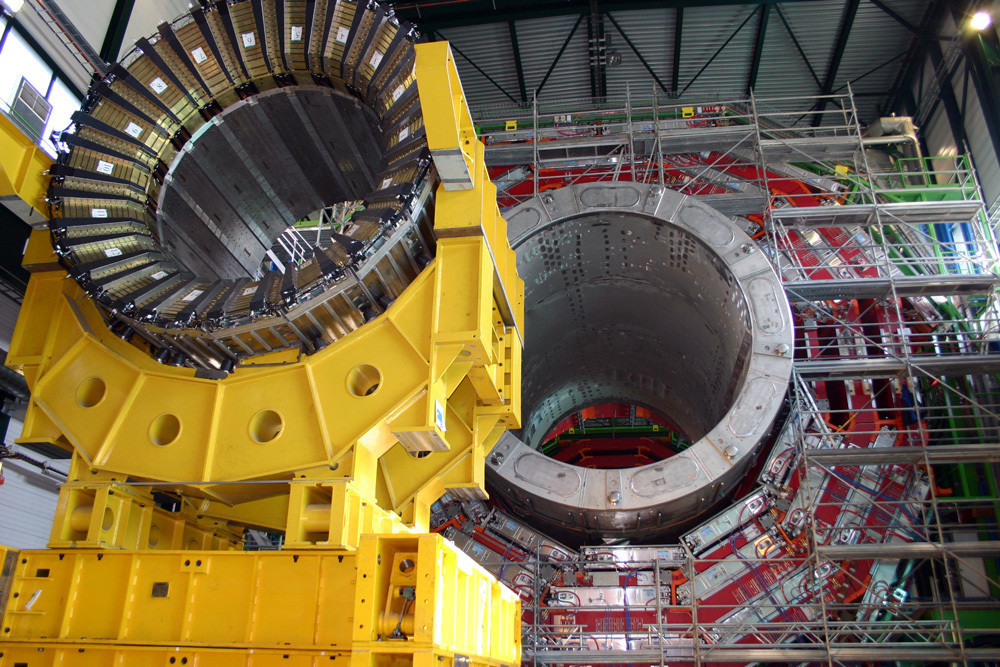
\includegraphics[width=0.45\textwidth,valign=c]{fig/cms/hcal_removed.jpg}\label{fig:cms_hcal_removed}}\quad
    \subfloat{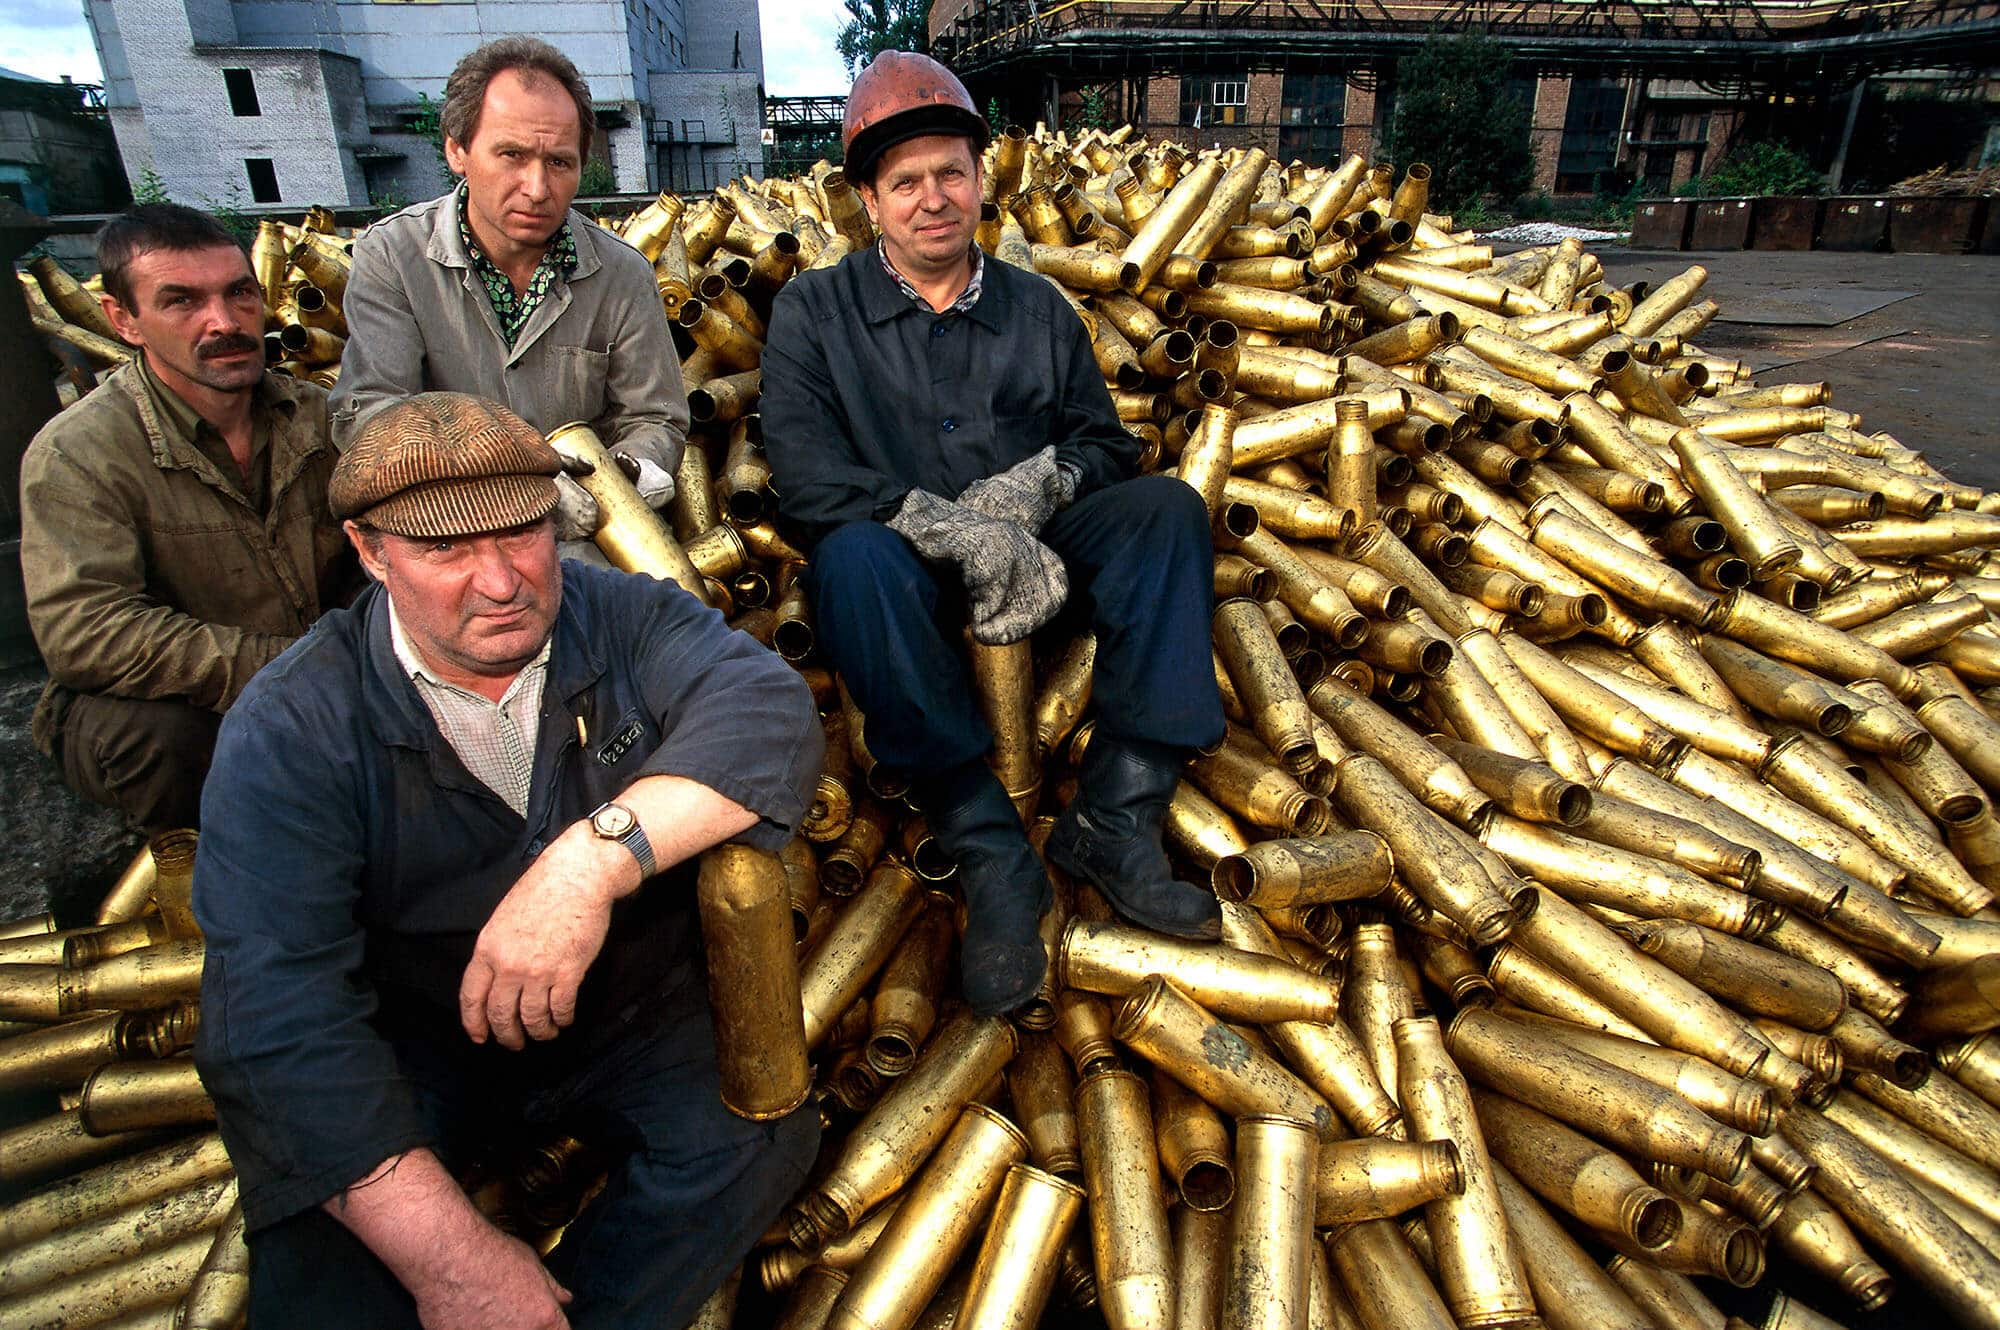
\includegraphics[width=0.45\textwidth,valign=c]{fig/cms/hcal_russian.jpg}\label{fig:cms_hcal_russian}}
    \caption{
        A photograph of the CMS hadronic calorimeter (HCAL) in front of the magnet and muon chambers before the detector was installed in the experiment cavern (left), from Ref.~\cite{Brice:1431485}, and workers in Mormansk sitting on the decomissioned World War II artillery shell casings used to supply the brass for the HCAL (right), from Ref.~\cite{GinterRussianDudes}.
    }
\end{figure}

\subsection{Muon chambers}
The CMS muon system (Fig.~\ref{fig:cms_subdetector_layout}) was originally composed of three different kinds of detectors: drift tubes (DTs) in the barrel, cathode strip chambers (CSCs) in the endcaps, and resistive plate chambers (RPCs) interwoven between the layers of DTs or CSCs. 
All of the different types of muon chambers operate on a similar principle: muons pass through a chamber filled with gas, liberating electrons from the gas atoms; those electrons are then collected on a conductive surface, resulting in an electric signal~\cite{CERN-LHCC-97-032}. 
The DTs (Fig.~\ref{fig:cms_muon_DT}) and CSCs are assembled into multiple layers that serve as an enormous outer tracker (Fig.~\ref{fig:cms_muon_stations}) exclusively for muons. 
DT and CSC modules also both have multiple inner layers in order to give a measurement of a muon's outer track accurate enough to be matched to its inner track in the silicon tracker. 
The RPCs, meanwhile, are designed to give a much faster, if less accurate, measurement of each muon's momentum. 
This measurement can be used to determine whether the pp collision is interesting or not.

\begin{figure}[htb]
    \centering
    \subfloat[]{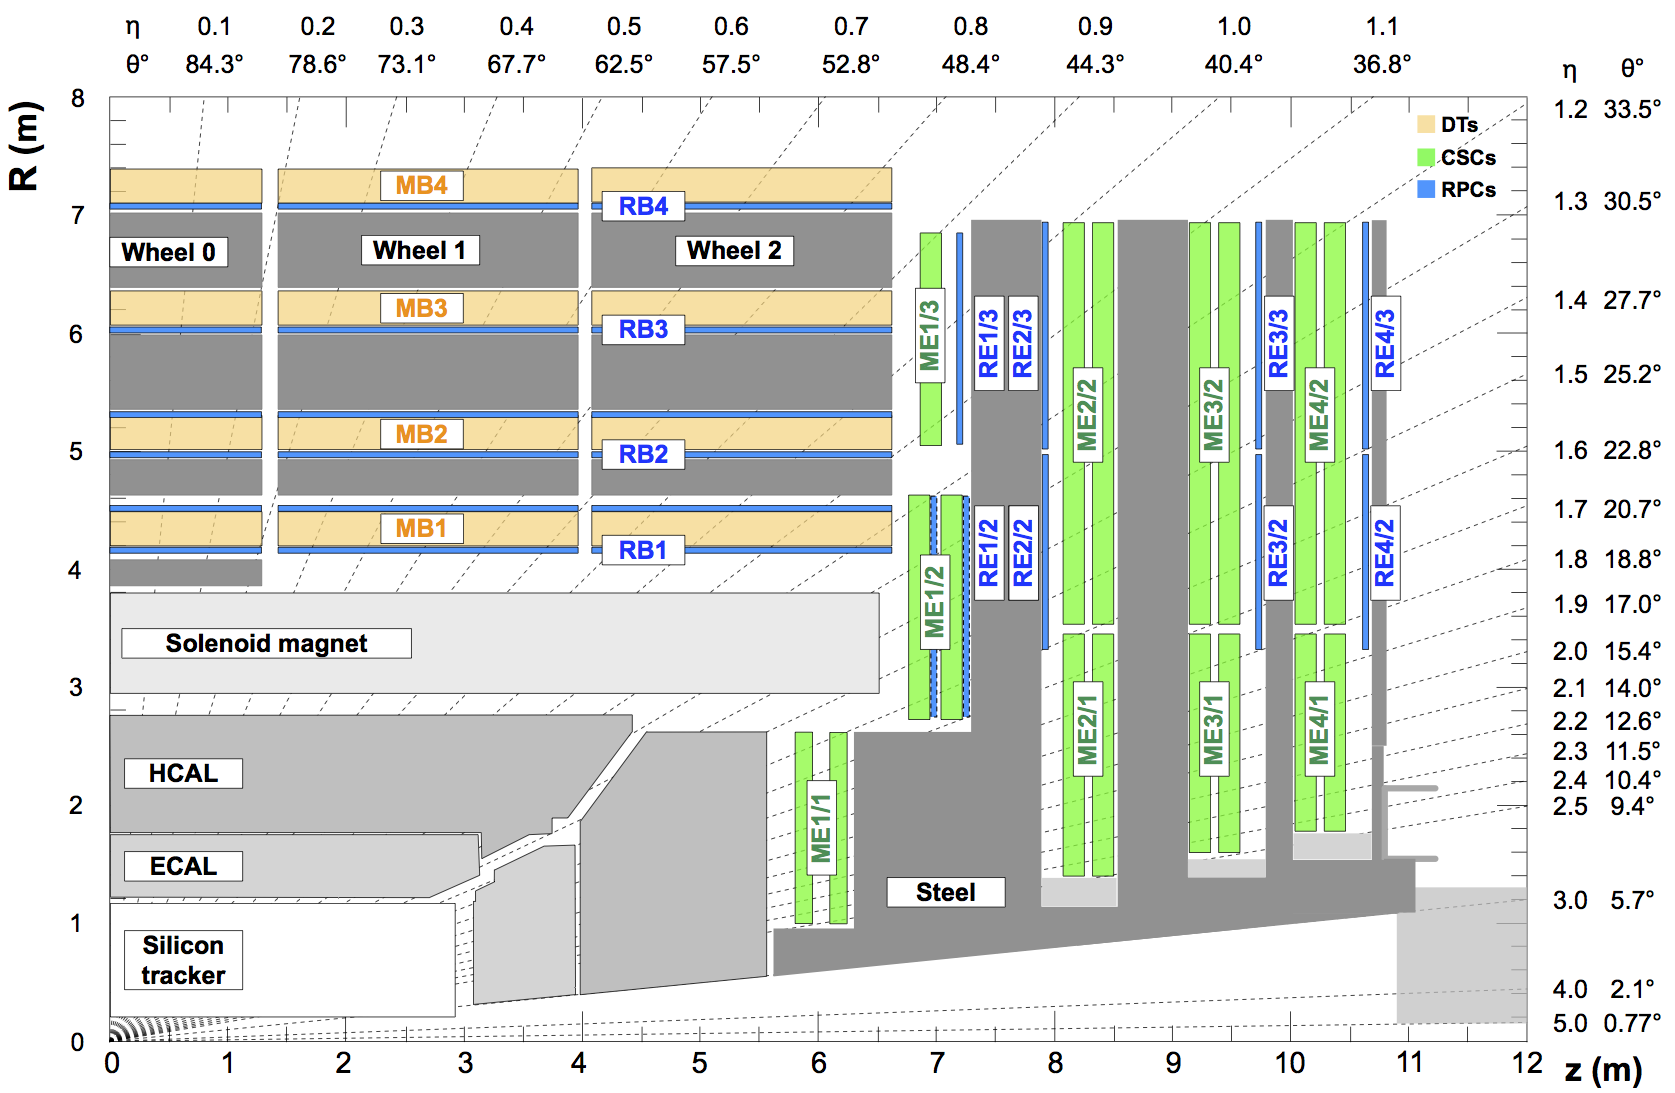
\includegraphics[width=0.6\textwidth,valign=c]{fig/cms/subdetector_layout.png}\label{fig:cms_subdetector_layout}}\quad
    \subfloat[]{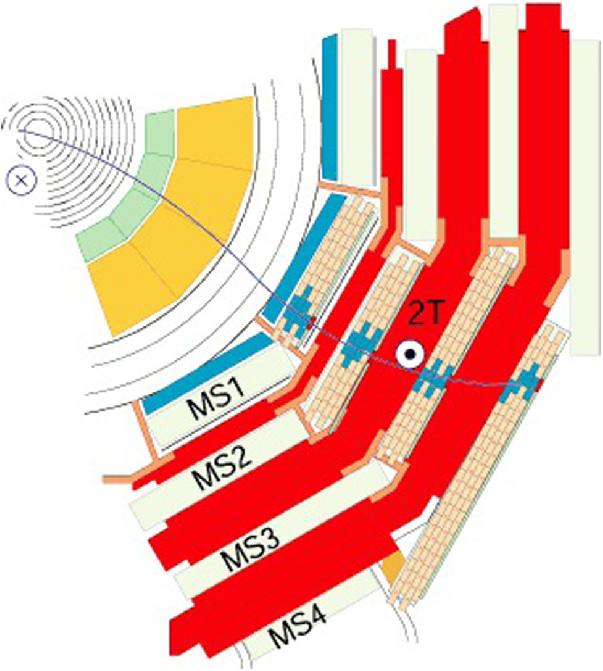
\includegraphics[width=0.3\textwidth,valign=c]{fig/cms/muon_stations.png}\label{fig:cms_muon_stations}}
    \caption{
        The cross section of CMS in the $r$-$z$ plane (left), from Ref.~\cite{CMS:2018rym}, and $r$-$\phi$ plane (right), from Ref.~\cite{CMSWebMuons}. 
        In the $r$-$z$ plane, the DTs, CSCs, and RPCs are drawn in light green, dark green, and blue, respectively, showing the layout of the muon system as well as the other subdetectors. 
        In the $r$-$\phi$ plane, the muon ``stations'' in the barrel are depicted with the DT internals exposed for stations with a throughgoing muon, showing the activation of the individual DT cells (blue) as well as the activiation of a section of the RPC (red).
    }
\end{figure}

\begin{figure}[htb]
    \centering
    \subfloat[]{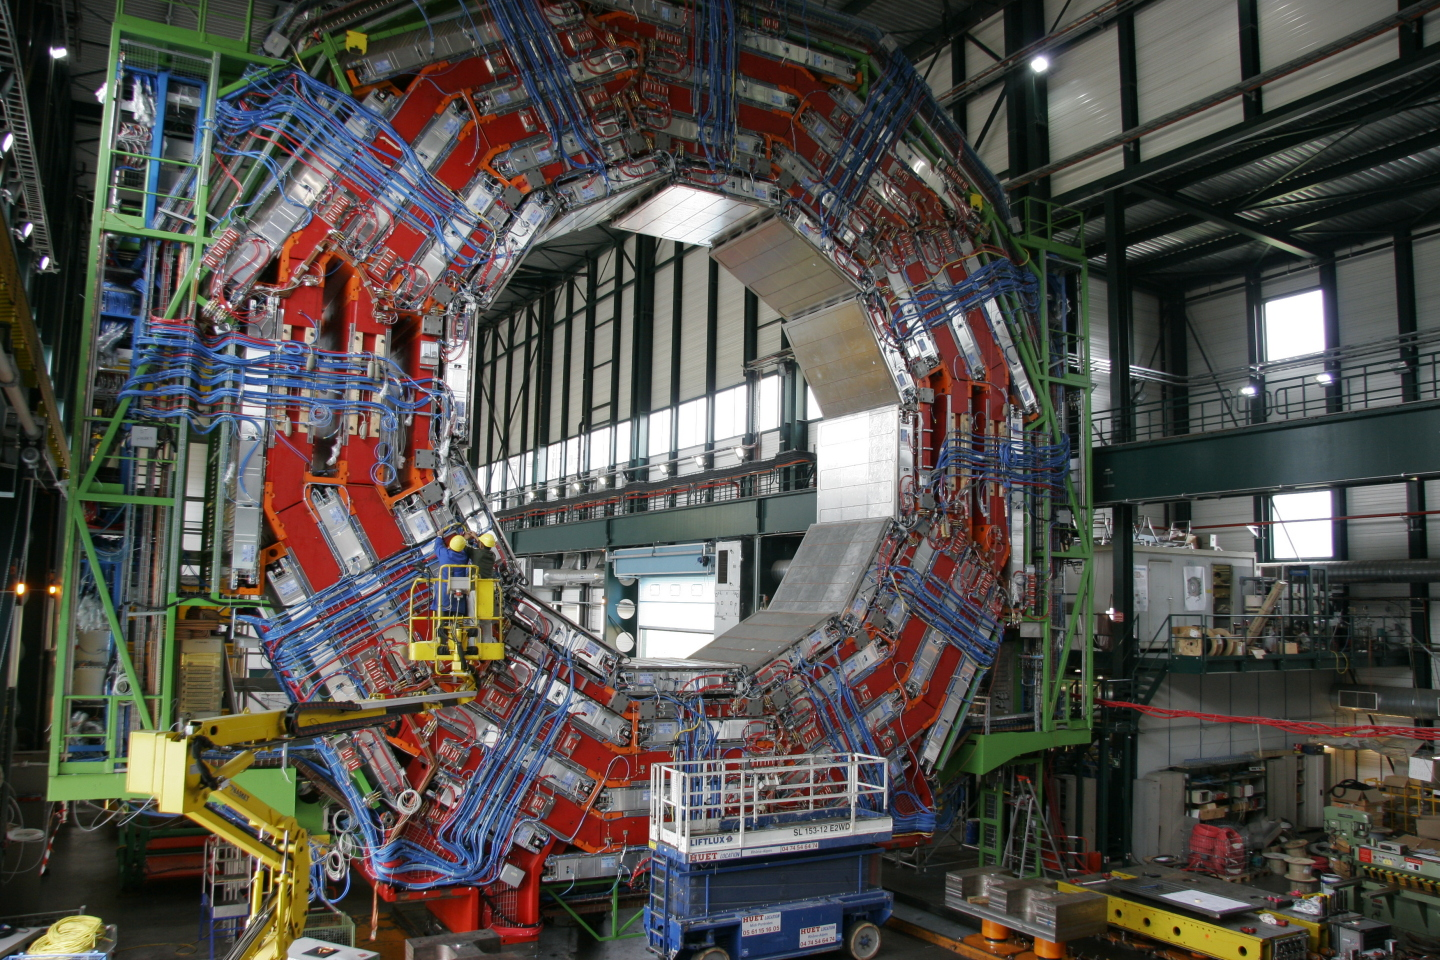
\includegraphics[width=0.465\textwidth,valign=c]{fig/cms/muon_DT_section.jpg}\label{fig:cms_muon_section}}\quad
    \subfloat[]{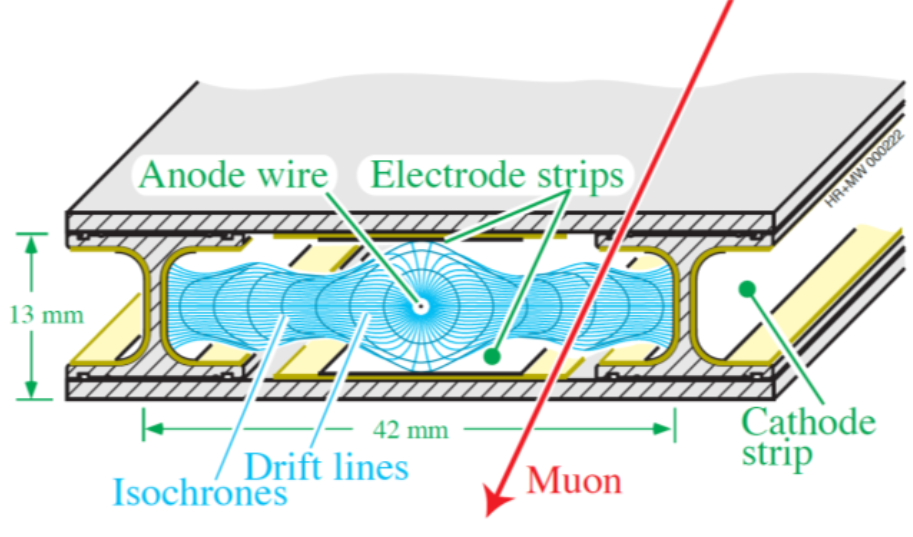
\includegraphics[width=0.435\textwidth,valign=c]{fig/cms/muon_DT_diagram.png}\label{fig:cms_muon_diagram}}
    \caption{
        A photograph of a section of the barrel muon chambers (drift tubes) before they were installed (left), from Ref.~\cite{Hoch:1274451}, and a diagram of a drift tube muon detector (right), from Ref.~\cite{CMSWebMuonDT}. 
    }
    \label{fig:cms_muon_DT}
\end{figure}

\clearpage

\section{The high lumonisity era}
There are three primary knobs to turn at the LHC: what things are being collided, what energy they are collided at, and how many of them are collided at once, or the luminosity. 
Since most of the experiments serviced by the LHC were designed for pp collisions, and because the LHC is designed only for 14\TeV collision energies, the final era of LHC physics will see a massive increase in luminosity. 
That is, at the ``high luminosity'' LHC (HL-LHC), there will be 100--200 concurrent pp collisions per bunch crossing (Fig.~\ref{fig:high_pu}), corresponding to an increase by a factor of 5--7.5.
More collisions means more opportunities for interesting physics. 
For example, in 2017, the LHC produced 3 million Higgs bosons per year, whereas the HL-LHC will produce over 15 million per year~\cite{HighLumiWebFacts}. 

\begin{figure}[htb]
    \centering
    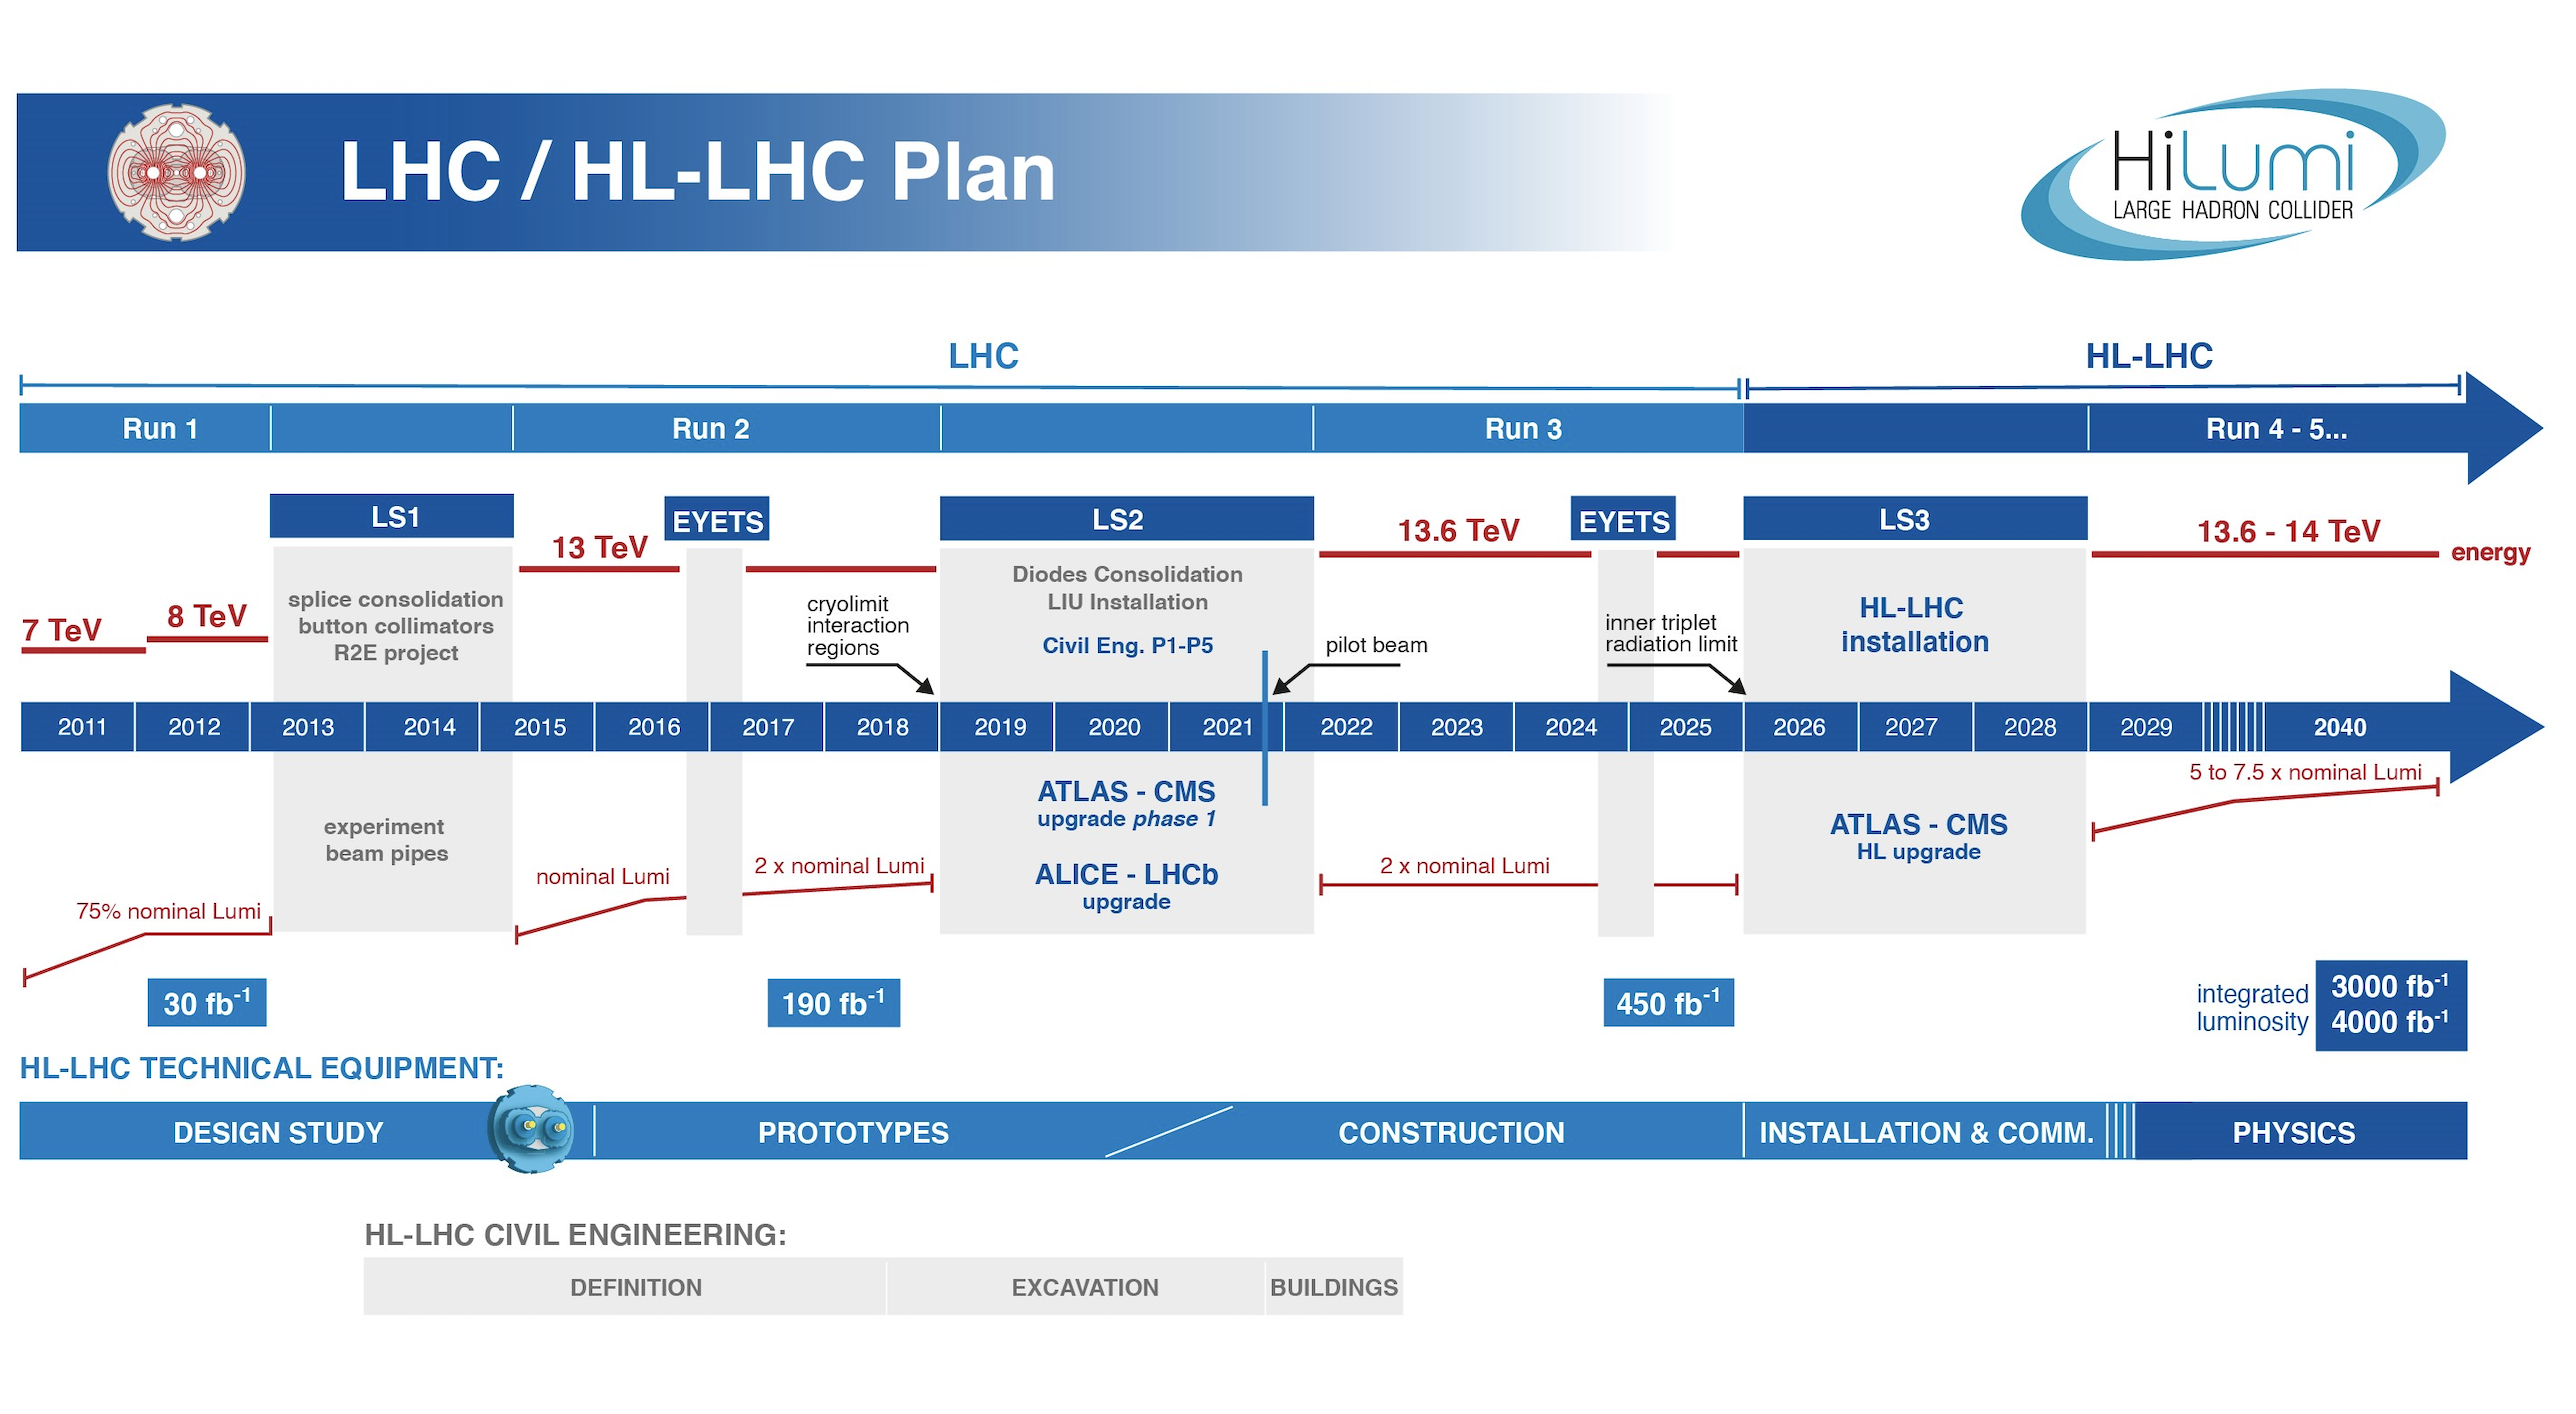
\includegraphics[width=0.9\textwidth,valign=c]{fig/lhc/hl_lhc_timeline.png}
    \caption{
        Lorem ipsum.
    }
    \label{fig:hl_lhc_timeline}
\end{figure}

\begin{figure}[!htb]
    \centering
    \subfloat[]{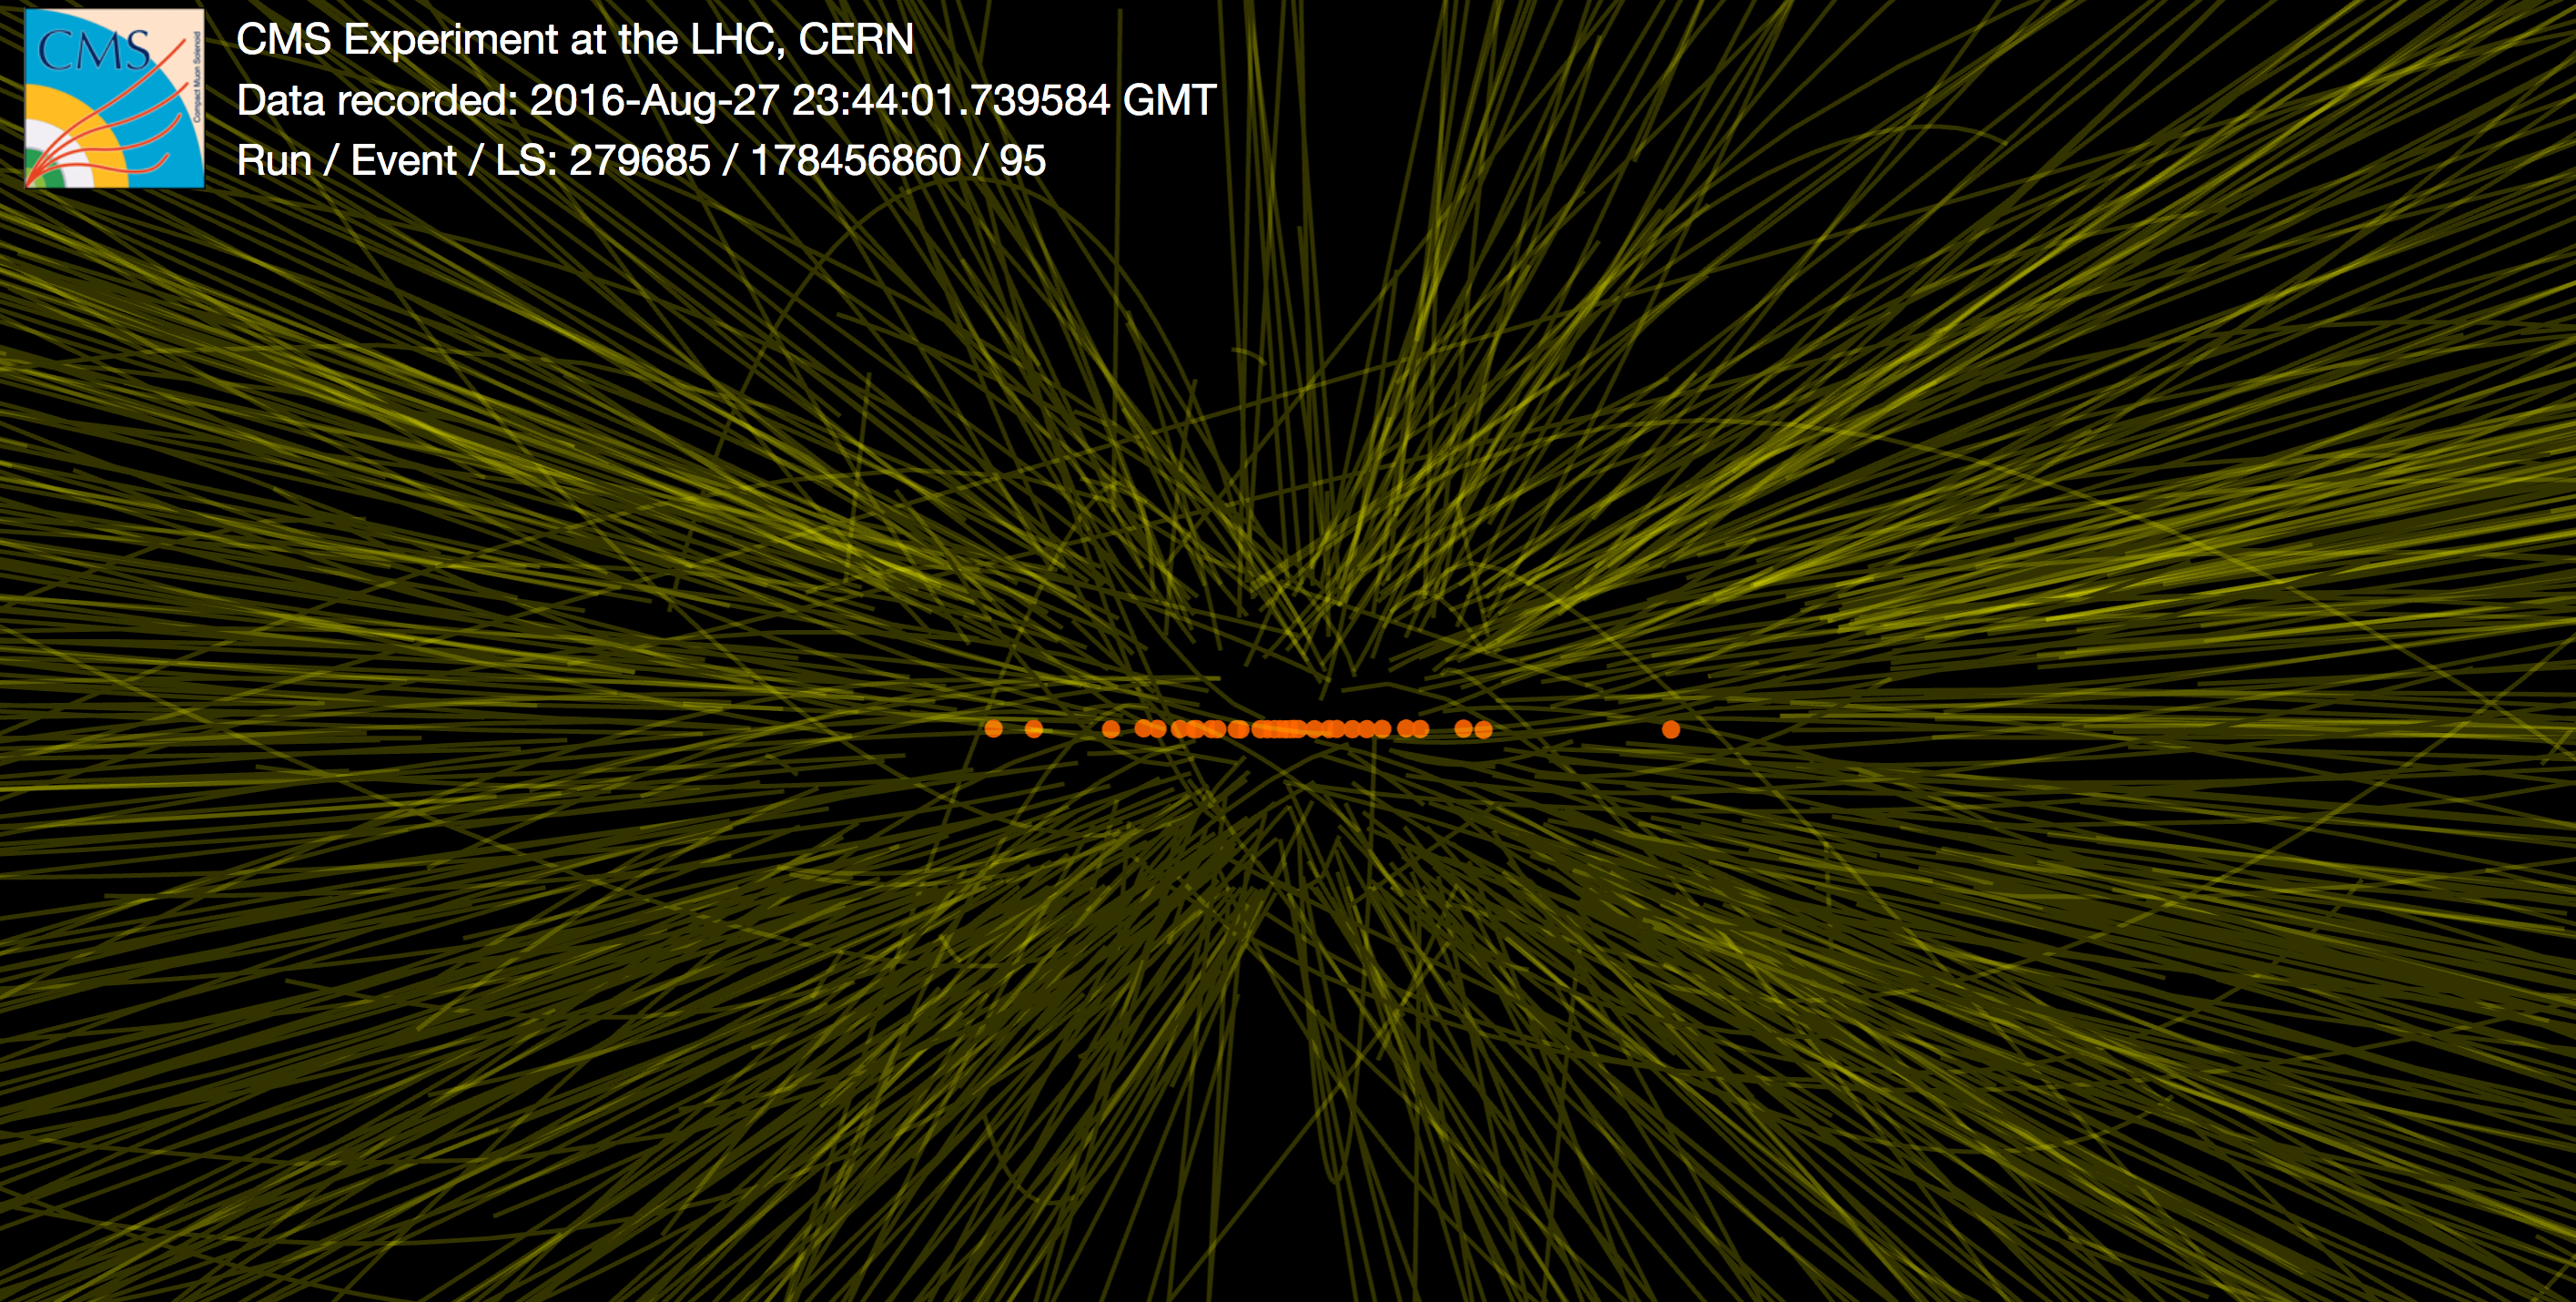
\includegraphics[width=0.45\linewidth]{fig/cms/high_PU_30vtx_side.png}\label{fig:normal_pu}}\qquad
    \subfloat[]{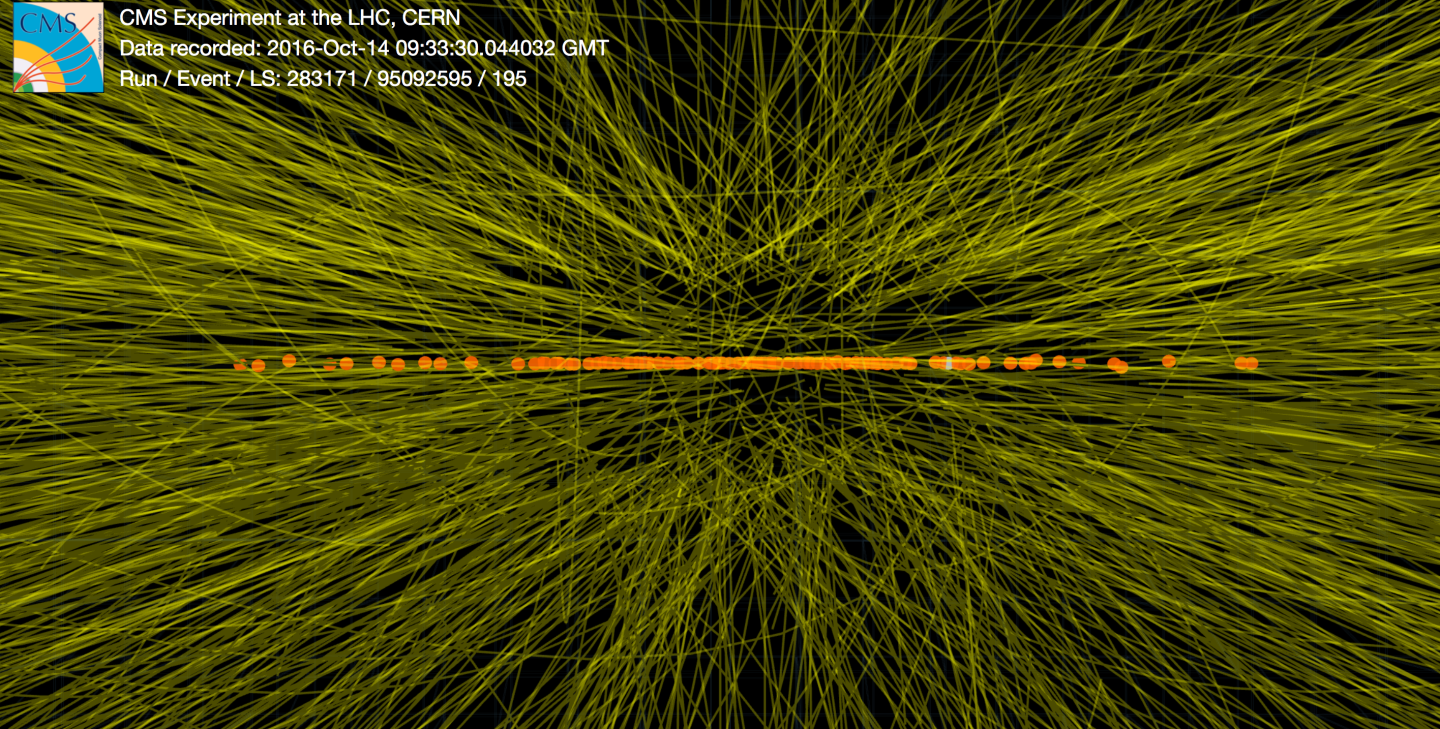
\includegraphics[width=0.45\linewidth]{fig/cms/high_PU_130vtx.png}\label{fig:high_pu}}
    \caption{
        A collision event with standard pileup (a) recorded at CMS in 2016 is shown next to an event with HL-LHC-like pileup (b) recorded at CMS in the same year, from Refs.~\cite{NormalPU2016, HighPU2016}.
        The dots are pp collisions and the thin lines are the reconstructed particle tracks.
    }
    \label{fig:pileup}
\end{figure}

\chapter{Studying the Higgs boson through vector boson scattering at CMS}\label{ch:higgs_vbs}
\begin{aquote}{Peter Higgs, Edinburgh University press conference, 2012}
    It's very nice to be right sometimes.
\end{aquote}

\section{New physics and the Higgs boson}
The stage is set: over a century of particle physics has yielded a beautiful theory of \textit{almost} everything, the Standard Model, and a grand coalition of nations has built the largest and most complex scientific instrument in human history, the LHC, to test it. 
The most recent act in this drama concluded in 2012, when the Higgs boson was discovered at CMS and ATLAS~\cite{CMSdisc, ATLASdisc}. 
In the years following its discovery, the LHC experiments have measured many of its properties to great precision and found no significant deviations from SM predictions~\cite{NatureHiggsCMS2022, NatureHiggsATLAS2022}. 
However, there are many features yet to be measured precisely. 
This implies that studies of the Higgs boson have incredible potential for discovery: a better understanding of the Higgs boson immediately yields a better understanding of the origin, operation, and continued existence of the entire universe. 
Moreover, the Higgs boson can uniquely interact with all known matter, so by producing many Higgs bosons in the lab, we may be able to access physics beyond the Standard Model (BSM). % citation needed

There are many educated guesses, called theories, on the answers to open question in particle physics, many of which involve the Higgs boson. 
Some guess at the existence of yet-undiscovered particles that also interact with the Higgs boson\footnotemark{}, and experimentalists can search for their existence directly: either by looking for the SM particles that they might decay into, or by checking for what is missing after everything is else accounted for. 
\footnotetext{This is not an unlikely guess: dark matter is known to have mass, and it may haved obtained that mass through the Higgs mechanism.}
Experimentalists can also search for new physics indirectly by making precise measurements of SM predictions; any significant deviation from the prediction would poke another hole in the Standard Model or even confirm a prediction of a new theory. 
The physics analyses described in this document both follow the latter strategy.

\subsection{The $\kappa$-framework}
One commonly used framework used to quantify these deviations from the SM is the so-called $\kappa$-framework~\cite{KFrame}, which introduces modifiers $\kappa_X$ to the Higgs boson couplings to some particle $X$:
\begin{equation}
    \kappa_X = \frac{\text{modifed coupling value}}{\text{SM coupling value}}.
\end{equation}
While there are myriad theoretical nuances to the statement above, it is sufficient to state the obvious: $\kappa_X = 1$ represents the SM scenario and significant deviations from 1 represent BSM scenarios. 
The $\kappa$-framework is not the only framework used to understand and quantify modifications to the SM, however, with the most notable alternative being Effective Field Theory~\cite{EFT, DimSix}. 

\section{Producing Higgs bosons with vector boson scattering}
The dominant Higgs boson production mechanism at the LHC is gluon-gluon fusion through a top quark loop. % TODO: add feynman diagrams, cite PDG?
Through these processes, the Higgs boson was discovered and many of its branching ratios and couplings have been measured precisely. 
However, additional production mechanisms can yield unique insights. 
Enter vector boson scattering\footnotemark{} (VBS), where two quarks scatter off of each other by the exchange of vector bosons ($\PV = \PW$ or \PZ). % TODO: add feynman diagram, ideally with "here there be monsters" circle with stuff coming out
\footnotetext{Although VBS specifically implies the production of two vector bosons, while vector boson fusion (VBF) implies the production of a single Higgs or vector boson~\cite{RauchVBSVBF2016}, the names VBS and VBF are used interchangeably; since we are interested in the production of a Higgs boson and one or two vector bosons, the naming is anyway ambiguous.}
This exchange can, in turn, produce a variety of physics, most notably the production of at least one Higgs boson. 
This process also has two important features. 
First, it has a unique signature: the two scattered quarks fly out of the collision back-to-back, typically in the forward regions of the detector (Fig.~\ref{fig:vbs_fireworks}), with a large combined invariant mass. 
Second, but equally important, modifications to the Higgs couplings induce effects that grow with energy~\cite{HiggsWithoutHiggs}---at the LHC, where energy is plentiful, this makes BSM scenarios easier to spot. 

\begin{figure}[htb]
    \centering
    \subfloat{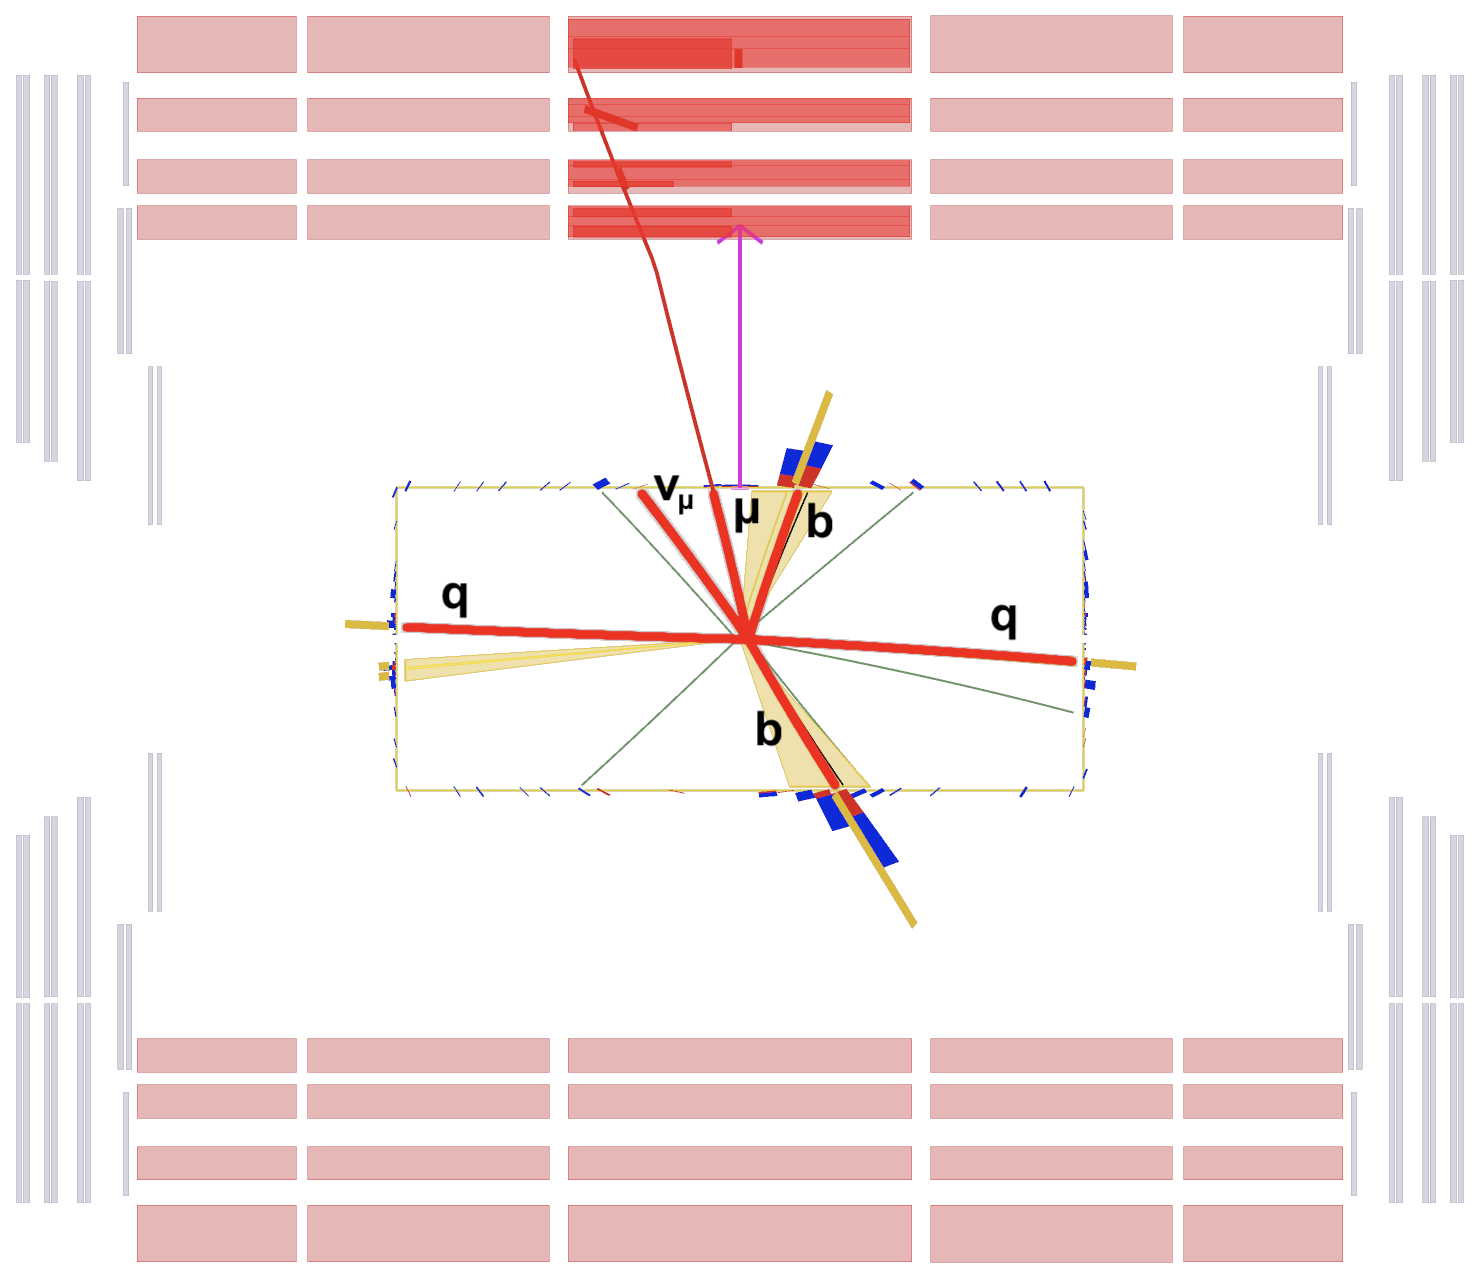
\includegraphics[width=0.45\textwidth]{fig/vbswh/fireworks/signal/vbswh_evt131104_rz_gen_labeled.png}}\qquad
    \subfloat{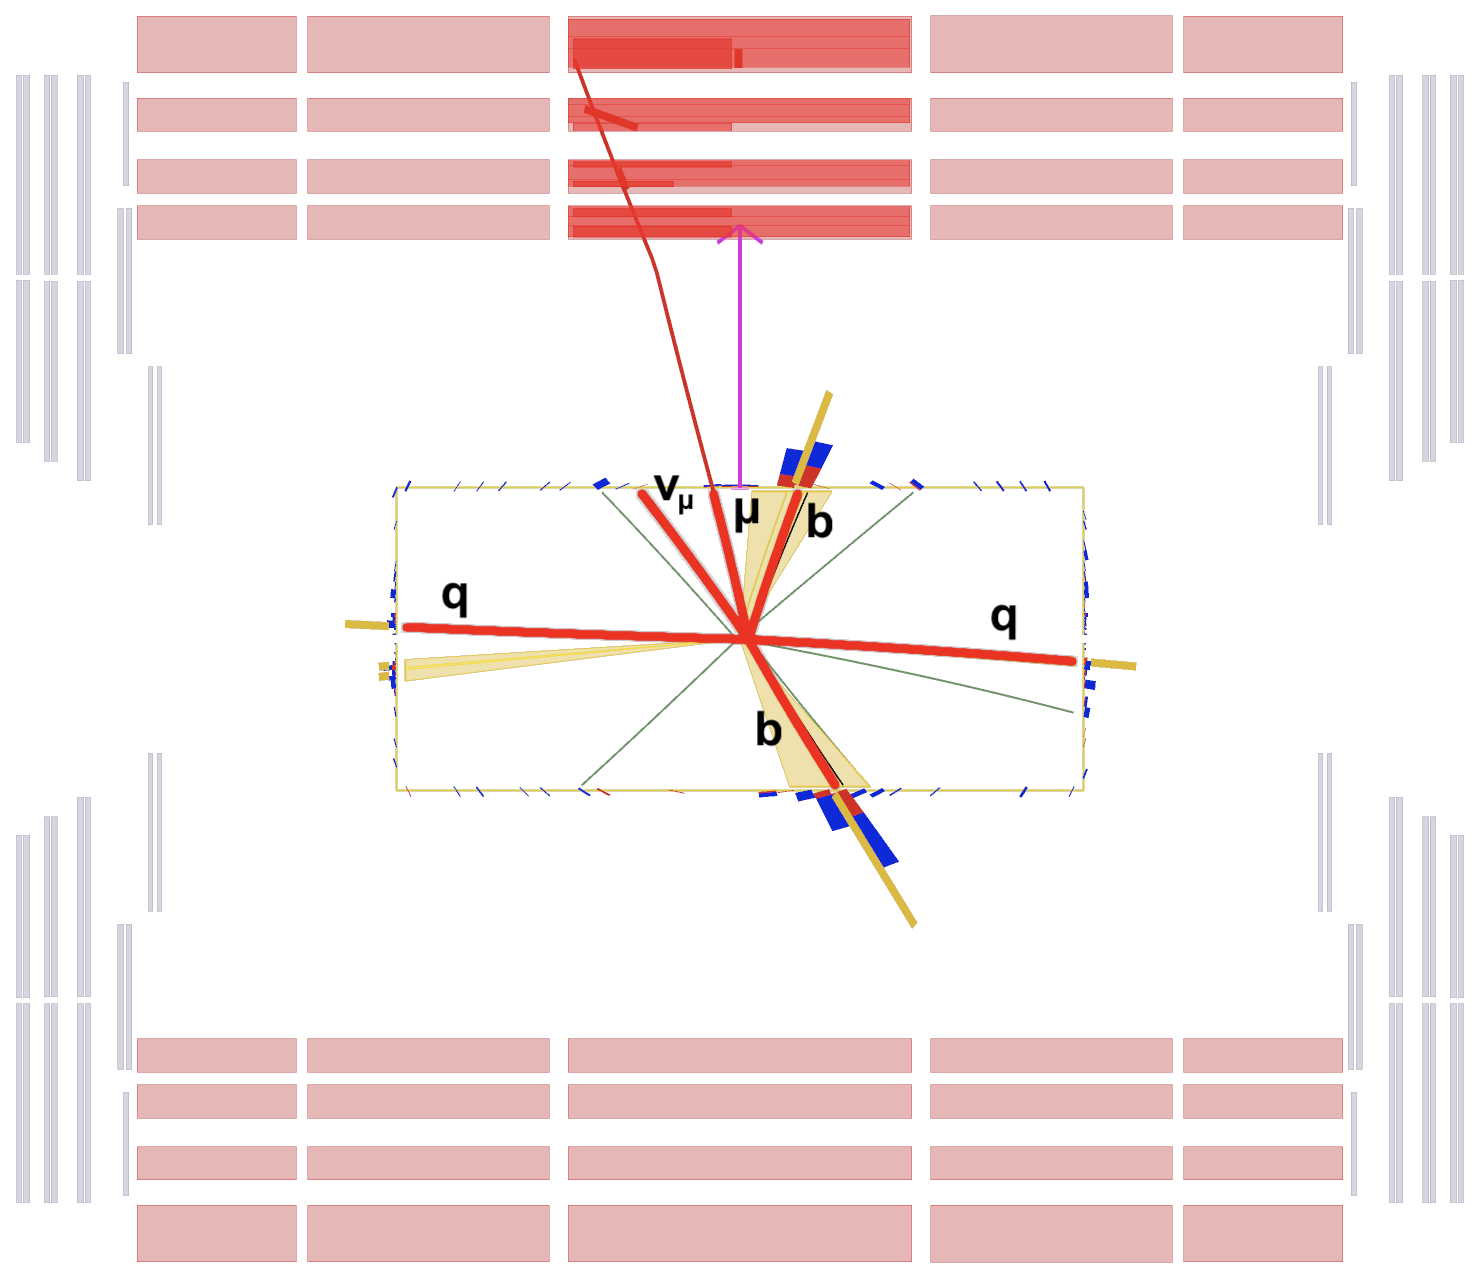
\includegraphics[width=0.45\textwidth]{fig/vbswh/fireworks/signal/vbswh_evt131104_rz_gen_labeled.png}} % TODO: label another plot, maybe VBSVVH, and replace this one
    \caption{
        Event display for a simulated VBS WH signal event. 
        The event is shown in the x-y plane (left) and x-z plane (right), and the final-state particles (thick red lines) are labeled with their true labels. 
        Two VBS jets can be seen very near to the beamline, going in either direction in $z$. 
    }
    \label{fig:vbs_fireworks}
\end{figure}

VBS provides a unique way of producing Higgs bosons, with an easily identifiable signature, and there are myriad VBS processes involving a Higgs, each involving different couplings. 
The rarer couplings are of particular interest, including the $\HHVV$ and $\HHH$ couplings (Ch.~\ref{ch:vbsvvh}). 
Also of interest are some of the more obscure properties of the Higgs boson, like the relative sign between the $\HWW$ and $\HZZ$ couplings (Ch.~\ref{ch:vbswh}). 
In all of these measurements, if we confirm SM predictions, we exclude possible BSM directions, and if find a significant deviation from the SM, we will have opened an entirely new chapter of physics. 

We begin by selecting the Feynman diagrams that involve the couplings of interest---here, we focus on VBS processes. 
We call the selected processes our ``signal.'' 
For example, if we are interested in $\HHVV$, as in Ch.~\ref{ch:vbsvvh}, our signal might be VBS production of a Higgs boson and two vector bosons. 
We must then find our signal, which is often incredibly rare, amongst petabytes of data recorded by CMS. 

\section{Choosing a final state}
The final collection of particles that are actually recorded by CMS are called the ``final state.'' 
As covered in Chapter~\ref{ch:lhc_cms}, Section~\ref{sec:cms}, CMS can record electrons, photons, hadrons, and photons. % TODO: continue; talk about how H and V decay, we choose those decays, etc.
All other SM particles---Higgs bosons, vector bosons, and gluons---decay to these particles, and we hope that BSM particles might as well. 
% However, the Higgs boson decays almost immediately to, in order of likelihood, quarks, leptons, a pair of vector bosons, or a pair of Higgs bosons.  
% Vector bosons, namely the \PW and \PZ bosons, similarly decay almost immediately to leptons, quarks, or a pair of vector bosons. 
% There are therefore a large variety of final states to choose from
% The presence of VBS quarks is therefore inferred from the presence of two jets, rather than neatly isolated objects, that are back-to-back. 
% The Higgs boson and vector bosons, meanwhile, decay almost immediately to quarks (which become jets), leptons (which \textit{are} nicely isolated objects), or sometimes to a pair of vector bosons\footnotemark{} (which again immediately decay). 
% \footnotetext{Of course, the Higgs boson can, uniquely, also decay to a pair of Higgs bosons through the $\HHH$ coupling.}
We must therefore decide on which Higgs boson and vector boson decays to target. 
For convenience, we often prefer to look for \Htobb, since that decay has the highest branching ratio (i.e. a Higgs boson is most likely to decay to a \bbbar). 
The choice for the decay of the vector bosons is less clear. 
The leptonic decays ($\PW\to\Pell\PGn$ or $\PZ\to\Pellp\Pellm$) are easier to spot, but are more rare. 
On the other hand, the hadronic decays ($\PV\to\qq$) are more plentiful, but are difficult to distinguish from far more abundant processes. 
In Chapter~\ref{ch:vbsvvh}, for example, there are two VBS jets, \bbbar from the Higgs, and a pair of quarks from the hadronic decay of each vector boson. 

\section{Common backgrounds}

\section{Isolating the signal}
With our signal selected, and the background composition understood, we may begin our analysis of the hundreds of petabytes of data collected by CMS. 
First, we try to ``reconstruct'' each particle produced in a given proton-proton collision, namely leptons and jets. 
Then, we develop an optimized selection strategy, using only simulated signal and background events to start, that picks out proton-proton collision events containing the final state of our signal. 
Once we are satisfied, we can count how many signal events we expect to pass our selection. 
We must also evaluate a thorough set of systematic uncertainties on that count. 
Depending on how we predict how many background events pass our selection, we may also need to evaluate systematic uncertainties on the background count. 
Finally, we take the expected signal count $S$ and predicted background count $B$ and compare them to the number of real proton-proton collisions that pass our selections. 
If the signal exists, then the real count should be roughly equal to $S+B$.
Otherwise, if we did our accounting correctly, the real count should be roughly equal to $B$. 
We use statistics (formally called ``hypothesis testing'') to do this comparison rigorously. 
The steps outlined here are detailed in the sections below. 
In Chapters~\ref{ch:vbswh} and \ref{ch:vbsvvh}, we will see them implemented in real analyses. 

\section{Reconstruction}

\begin{figure}[htb]
    \centering
    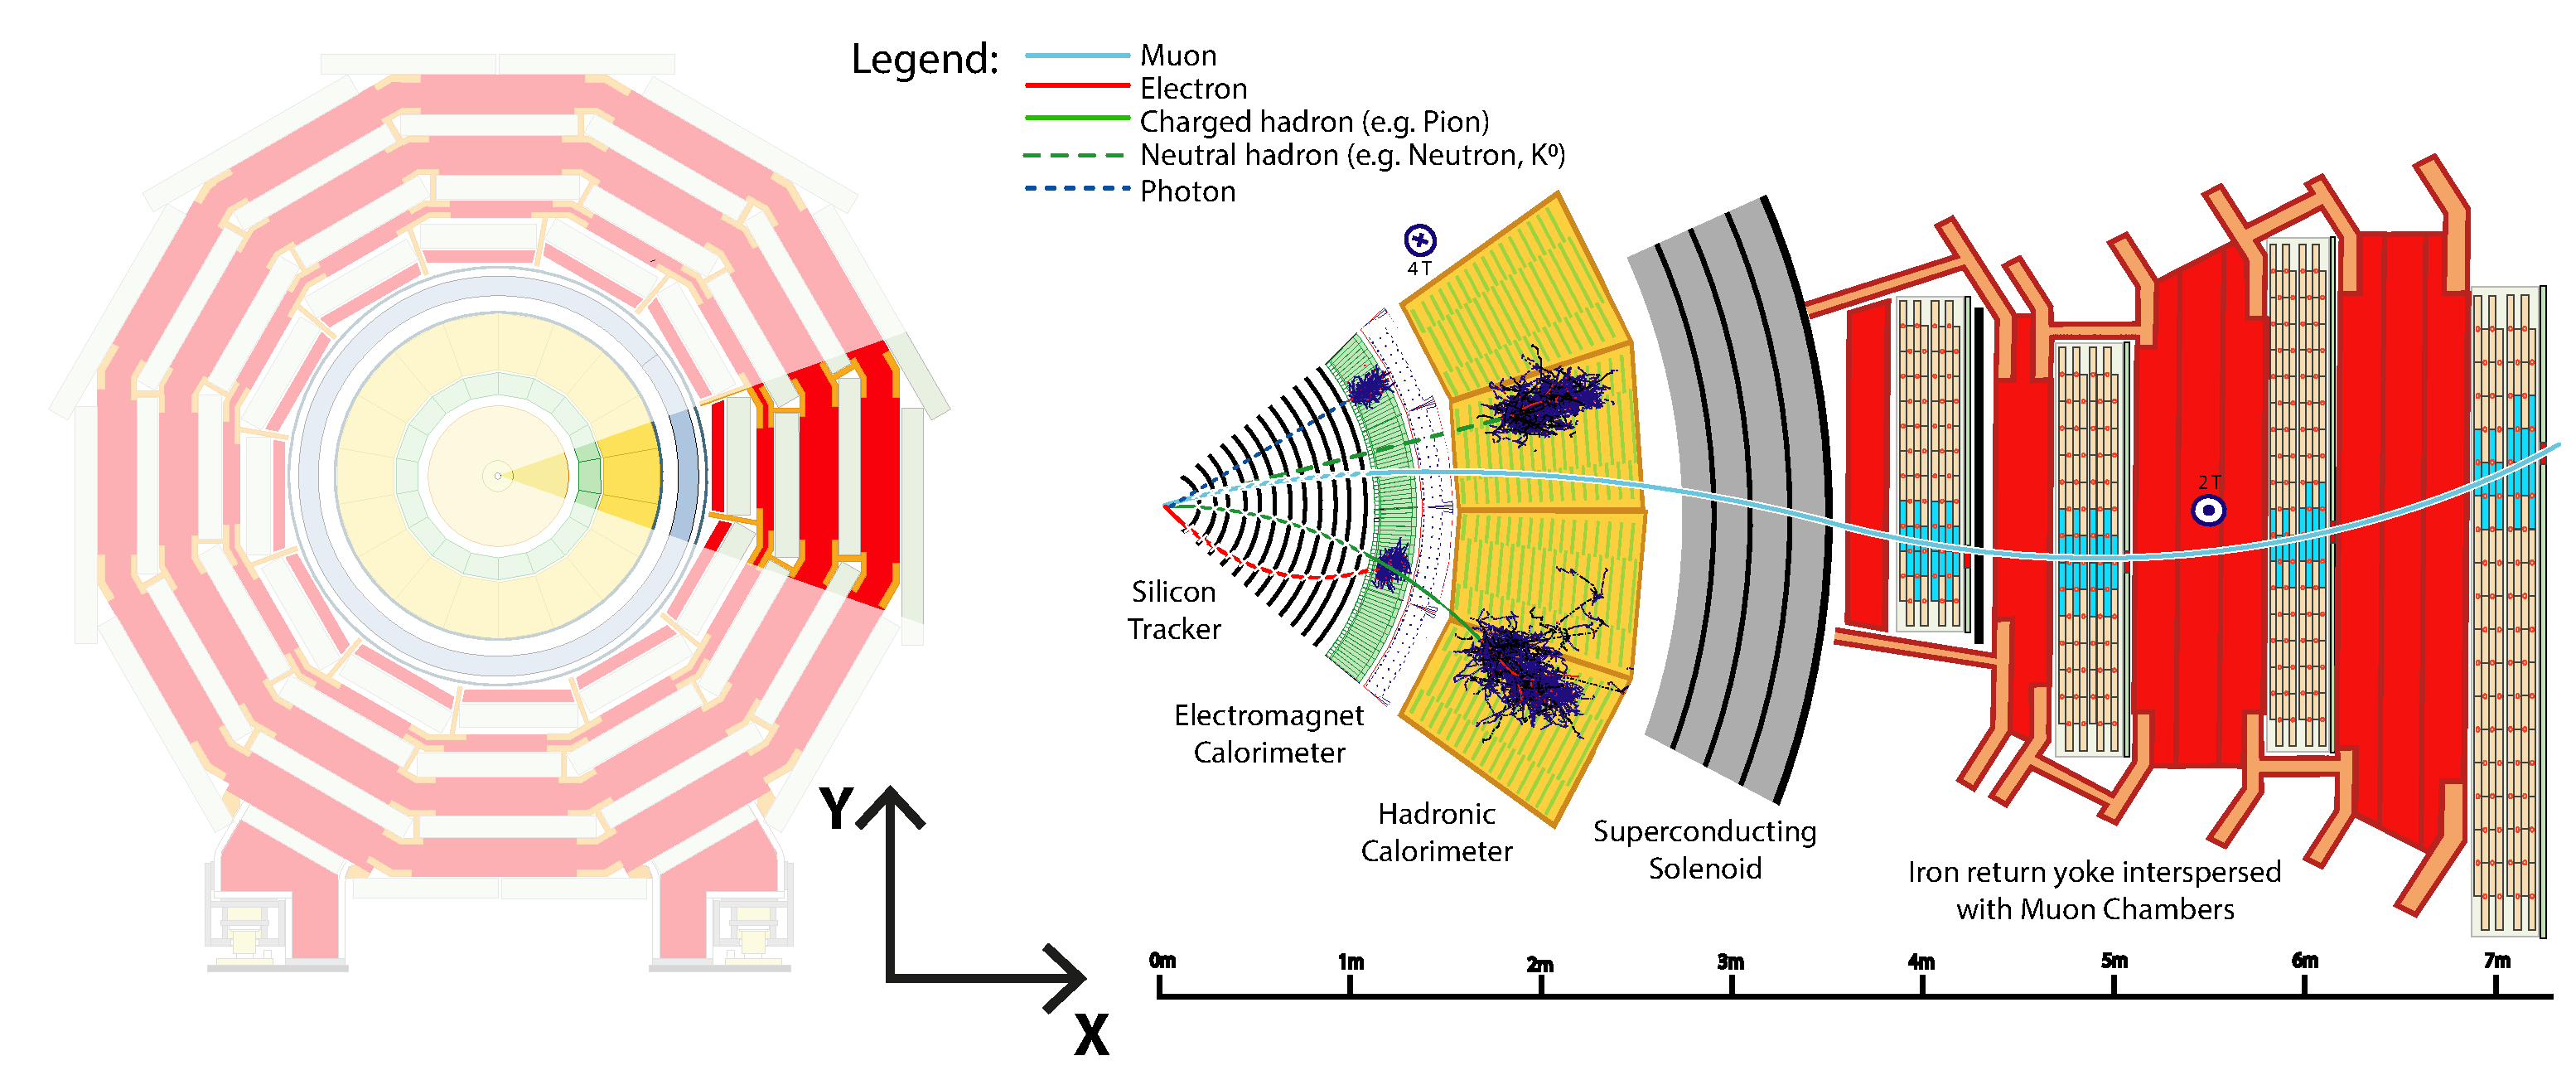
\includegraphics[width=0.95\textwidth]{fig/cms/particle_id_slice.pdf}
    \caption{
        Transverse slice of CMS, from Ref.~\cite{Davis:2205172}, showing the signals left by different kinds of particles in each subdetector.
    }
    \label{fig:cms_particle_id}
\end{figure}

\subsection{Leptons}
\subsubsection{Electrons and muons}
\subsubsection{Tau leptons}
\subsubsection{Neutrinos}

\subsection{Jets}
Due to quark ``confinement,'' quarks hadronize into ``jets'' of hadrons. 
This happens in a cascade, where quarks beget quarks that beget more quarks and so on, until the jet impinges on the calorimeters. 

\subsubsection{Jets originating from VBS quarks}\label{sec:vbsjets}
The presence of VBS quarks is inferred from the presence of two jets that are back-to-back. % TODO: add event display or something showing this, maybe detajj histogram

\subsubsection{Jets originating from b quarks}

\section{Simulation}

\section{Event selection}
In order to isolate the signal, we must place a set of selections on our data that prefer events that look like signal. 
We do this in a particular order, however, because of the sheer size of our data. % TODO: maybe add a diagram here, showing some sort of cut flow or logical flow for data and MC

\subsection{Triggers}
We first select the HLT paths most relevant to the chosen final state. 
For example, if the final state includes one lepton---say, from the leptonic decay of a \PW boson---then then we would select the single-lepton HLT paths. 
This isolates a portion of the petabytes of CMS data that are relevant for analysis. 
The HLT paths are also implemented in the simulation, so we will require that simulated events pass the same HLT paths as the data. 

\subsection{Signal regions}
\subsection{Control regions}
\subsection{Background estimation}

\section{Systematic uncertainties}
Since the background estimation strategy is data-driven, the systematics on the Monte Carlo, which are more numerous, only need to be evaluated for the signal yield. 
Most sources of systematic uncertainty are derived by varying individual theoretical scales and experimental corrections by one standard deviation and taking the maximal difference in yield as the error. 
In particular, the corrections and their uncertainties are typically derived centrally in order to augment the efficiency of a specific selection in MC to match that measured in data.
In general, these corrections are applied as an event weight $\omega$, such that the weighted contribution $\Omega$ of each raw Monte Carlo event is given by the product of the event weights for that same event. 
The yield in a given signal region $y$ containing $N$ raw Monte Carlo events is therefore given by
\begin{equation}
    y = \sum_{i = 1}^{N}\Omega_i
\end{equation}
Then, the yield $y_\text{var}$ is computed after applying a systematic variation (up or down) of each source of systematic uncertainty independently:
\begin{equation}\label{eq:systs}
    y_\text{var} = \sum_{i = 1}^{N}\Omega_i\times\frac{\omega_\text{var}}{\omega}
\end{equation}
Finally, the maximum of the percent differences $\delta_\text{up}$ or $\delta_\text{down}$ are taken as the systematic uncertainty for that source, where
\begin{equation}
    \delta_\text{var} = \bigg| 1-\frac{y_\text{var}}{y} \bigg|
\end{equation}

\section{Statistical interpretation}
\subsection{Maximum likelihood estimate}

\chapter{Determination of $\lambda_\text{WZ}$ through VBS WH production}\label{ch:vbswh}

\section{Looking for a sign}
Before this work was published, the CMS Collaboration had measured the \textit{magnitudes} of the HWW (\kW) and HZZ (\kZ) couplings to be $\abs{\kW} = 1.02^{+0.11}_{-0.10}$ and $\abs{\kZ} = 1.04^{+0.07}_{-0.07}$, showing precise agreement with the SM values~\cite{NatureHiggsCMS2022}---with similarly strong constraints from ATLAS~\cite{NatureHiggsATLAS2022}. 
The \textit{sign} of either coupling, however, had not yet been well-determined. 
The relative sign between \kW and \kZ, which was of particular interest, can be expressed more compactly as the ratio between the two couplings:
\begin{equation}
    \lambdaWZ = \frac{\kW}{\kZ}.
\end{equation}
The Standard Model requires $\lambdaWZ = 1$ in order to preserve the ``custodial'' symmetry. 
Meanwhile, certain BSM theories require \lambdaWZ to be negative~\cite{Theory1LambdaWZ}, including models with higher isospin representations~\cite{Low2010} like the Georgi-Machacek model~\cite{GEORGI1985463}. 
Therefore, in the absence of a significant experimental measurement of the sign of \lambdaWZ, a crucial element of the SM had not been confirmed, and a potential signature of BSM physics was left unexplored. 

\section{The signal}
The precise determinations of the magnitudes of \kW and \kZ~\cite{NatureHiggsCMS2022} were obtained in studies of processes that are predominantly quadratic in \kV---that is, \kW or \kZ enter the Feynman diagram twice. % add a feynman diagram?
While there were some with a linear dependence, they did not give a strong exclusion of opposite-sign scenarios~\cite{BestCMSLambdaWZ}---in fact they slightly preferred the $\lambdaWZ < 0$ scenario. 
A promising channel to directly probe \lambdaWZ at the LHC is the production of \VH via vector-boson scattering (VBS)~\cite{Theory2LambdaWZ}, shown (at leading order) in Fig.~\ref{fig:vbswh_feynman}.
Such a channel is sensitive to the relative sign of \kW and \kZ since the cross-section $\sigma$ has an interference term that is linear in both \kW and \kZ~\cite{Theory2LambdaWZ}: 
\begin{equation}\label{eq:vbswh_matrix_elem}
    \sigma \propto \abs{\mathcal{M}}^2 = \kW^2\abs{\mathcal{M}_W}^2 + \kW\kZ\mathcal{M}_{WZ}^2 + \kZ^2\abs{\mathcal{M}_Z}^2
\end{equation}
where the matrix elements for the contributions from the HWW couplings, HZZ couplings, and interference term are denoted as $\mathcal{M}_W$, $\mathcal{M}_W$, and $\mathcal{M}_{WZ}$, respectively. 
Therefore, this channel provides the opportunity to determine the sign of \lambdaWZ. 
\begin{figure}[htb]
    \centering
    \subfloat{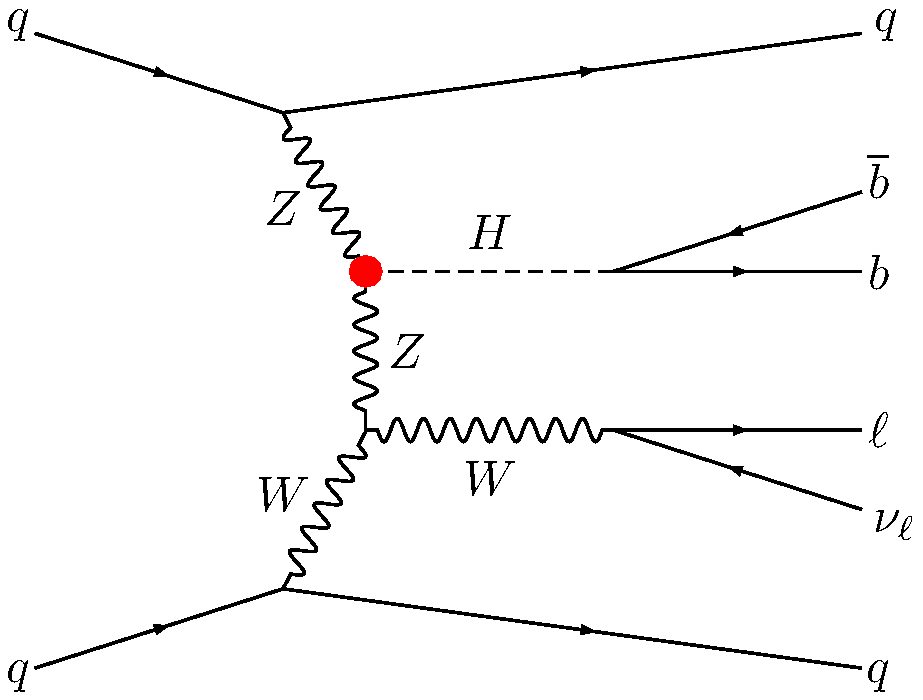
\includegraphics[width=0.3\textwidth]{fig/feynman/vbswh/vbswh_1.pdf}}\quad
    \subfloat{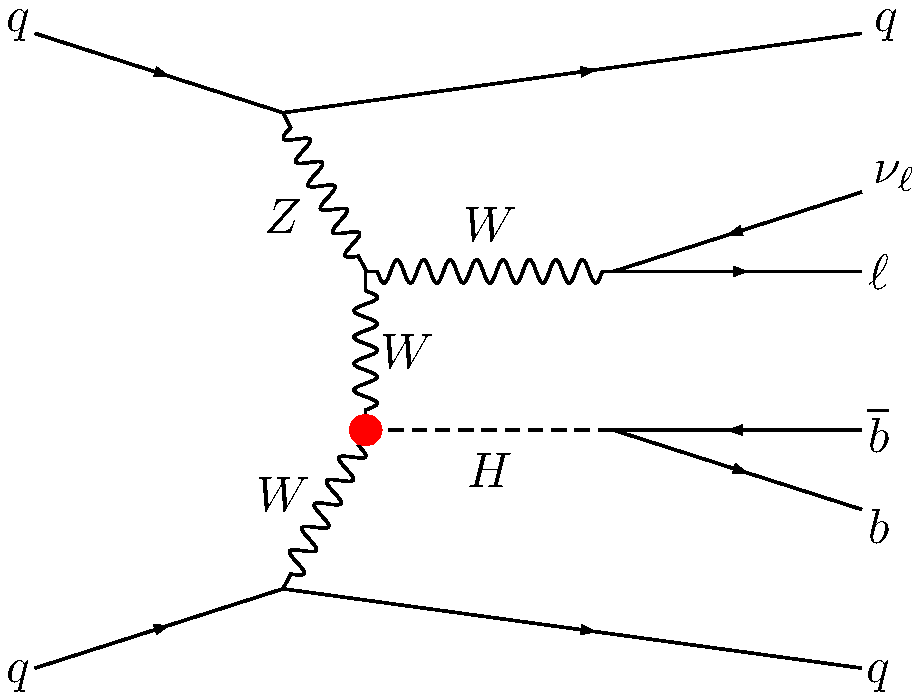
\includegraphics[width=0.3\textwidth]{fig/feynman/vbswh/vbswh_2.pdf}}\quad
    \subfloat{\includegraphics[width=0.3\textwidth]{fig/feynman/vbswh/vbswh_3.pdf}}
    \caption[Leading-order Feynman diagrams for VBS \WH production]{
        Leading-order Feynman diagrams for VBS production of a W and Higgs boson, where the W decays leptonically and the Higgs decays to b quarks. 
        The Higgs coupling to W bosons \kW and Z bosons \kZ is denoted by a red circle (\textcolor{red}{\ding{108}}). 
    }
    \label{fig:vbswh_feynman}
\end{figure}

\subsection{Signal characteristics}
A specific final state is intentionally selected for its uniqueness---making the signal easier to find amidst the haystack. 
First, leptons are preferred in the final state over jets, due to the sheer size of the ``QCD multijet'' background, the most populous physics process produced at the LHC where the interactions between the quarks and gluons in the colliding protons simply produce more quarks and gluons. 
Then, $\PW\to\ell\nu$ is preferred over $\PZ\to\ell\ell$, since there are fewer backgrounds with only one lepton in the final state. 
Finally, $\PH\to\PQb\PAQb$ has the largest branching ratio, and it can be identified using the latest advances in artificial intelligence. 

While there are a few, quite large background processes can produce the target final state, the Monte Carlo (MC) simulation of the signal reveals additional boons. 
The final state particles receive a significant boost for negative \lambdaWZ scenarios (Fig.~\ref{fig:vbswh_lhe}). 
In our preferred final state, this will give a lepton with large \pt, some additional \MET from the neutrino, and two overlapping b-jets reconstructed as a single merged jet. 
This can be quantified in a single variable by simply summing the \pt of each final-state particle other than the VBS jets:
\begin{equation}\label{eq:vbswh_st}
    \ST = \pt(\PW\to\ell\nu)+\pt(\Htobb) = \pt(\ell)+\ptmiss+\pt(\text{AK8 jet})
\end{equation}
The cross-section of the signal process increases almost quadratically as \kW or \kZ deviate from the SM value (Fig.~\ref{fig:vbswh_xsecs}), so there are simply more signal events in BSM scenarios. 
Importantly, the cross-section and Lorentz boost are the same for $\kW=-1$, $\kZ=1$ and $\kW=1$, $\kZ=-1$. 
The analysis was optimized for the latter case. 

\begin{figure}[htb]
    \centering
    \includegraphics[width=0.45\textwidth]{fig/vbswh/lhe_ST_kWpoints.pdf}\label{fig:lheST_kWpoints}
    \caption[Generator-level \ST distribution]{
        Distribution of \ST plotted at the generator level for $\kZ = +1$, demonstrating the Lorentz boost in the final state due to modifications to \lambdaWZ. 
        Importantly, the distributions look identical for the case where $\kW = +1$ and \kZ is similarly varied.
    }
    \label{fig:vbswh_lhe}
\end{figure}

\begin{figure}[htb]
    \centering
    \subfloat{\includegraphics[width=0.45\textwidth]{fig/vbswh/kW_xsecs.pdf}}
    \qquad
    \subfloat{\includegraphics[width=0.45\textwidth]{fig/vbswh/kZ_xsecs.pdf}}
    \caption[The signal cross-section plotted as a function of enhancements to \kW]{
        The signal cross-section plotted as a function of enhancements to \kW, keeping $\kZ = +1$ (left) and to \kZ, keeping $\kW = +1$ (right). 
        The black points are taken from \MGvATNLO, and the blue curve is the best fit of a 2nd order polynomial to those points. 
    }
    \label{fig:vbswh_xsecs}
\end{figure}

The VBS jets also provide a distinct kinematic signature (Fig.~\ref{fig:vbswh_fireworks}), namely two nearly back-to-back jets---i.e. a large absolute difference in pseudorapidity \abs{\detajj}---with a large combined invariant mass \Mjj. 
In particular, the background processes fall off exponentially in \Mjj whereas the signal process is more flatly distributed. 
Combined with the fact that the signal has a distinctly larger average value of \abs{\detajj} than background, these VBS characteristics form a strong handle for distinguishing signal from background. 

\begin{figure}[htb]
    \centering
    \subfloat{\includegraphics[width=0.45\textwidth]{fig/vbswh/fireworks/signal/vbswh_evt131104_rphi_gen_labeled.png}}
    \qquad
    \subfloat{\includegraphics[width=0.45\textwidth]{fig/vbswh/fireworks/signal/vbswh_evt131104_rz_gen_labeled.png}}
    \caption[Event display for a simulated VBS \WH event]{
        Event display for a simulated VBS \WH event in the $r$-$\phi$ plane (left) and $r$-$z$ plane (right), with the final-state particles (thick red lines) labeled. 
        Two VBS jets can be seen very near to the beamline, going in either direction in $z$. 
    }
    \label{fig:vbswh_fireworks}
\end{figure}

\section{The backgrounds}
In general, background processes for this analysis need a fake\footnotemark{} $\Htobb$ merged jet, two fake\footnotemark[\value{footnote}] VBS jets, one lepton, and some \MET. 
\footnotetext{
    In principle, a background process could have a \textit{real} Higgs boson with large \pt decay to \bbbar or two \textit{real} VBS jets, however SM processes with these kinds of signatures are so rare that they do not represent a significant background for this analysis.
}
The leading background process for this analysis is \ttbar production, wherein a top and antitop quark are produced and both decay to a bottom quark and \PW boson. 
One of the \PW bosons can decay to a real lepton and neutrino, and the fake VBS jets and \Htobb merged jet can come from some combination of the \PQb quarks, quarks from one of the \PW bosons decaying hadronically, and possibly an extra gluon radiated by one of the incoming quarks (Fig.~\ref{fig:ttbar1l}). 
One of the incoming quarks can also radiate a \PW or \PZ boson (Fig.~\ref{fig:ttV1l}), which presents additional opportunities for trickery. 
The largest sub-leading background comes from \wjets (Fig.~\ref{fig:w_jets}), where a \PW boson is produced along with some number of quarks or gluons, and single-top production (Fig.~\ref{fig:single_t}), where only one top quark is produced. 
In \wjets, the W can give a real lepton and neutrino, while the additional jets cover the fake VBS and \Htobb signature. 
In single-top production, the top quark again decays to a \PW boson and b quark, so it can produce a signal-like final state much like \ttbar. 

\begin{figure}[htb]
    \centering
    \subfloat[$\ttbar + \text{jet}$]{\includegraphics[width=0.4\textwidth]{fig/feynman/ttbar/ttbar_onelep_extraJet_ggF.pdf}\label{fig:ttbar1l}}
    \quad
    \subfloat[$\ttbar + \PV$]{\includegraphics[width=0.4\textwidth]{fig/feynman/ttbar/ttV_onelep.pdf}\label{fig:ttV1l}}
    \\
    \subfloat[\wjets]{\includegraphics[width=0.4\textwidth]{fig/feynman/other/wjets.pdf}\label{fig:w_jets}}
    \quad
    \subfloat[Single top]{\includegraphics[width=0.4\textwidth]{fig/feynman/other/singletop_tW.pdf}\label{fig:single_t}}
    \caption[Feynman diagrams the leading (\ttbar) and subleading (\wjets and single top quark) backgrounds]{
        Feynman diagrams for the leading and subleading backgrounds in this analysis.
        From top to bottom: 
        \ttbar production in the single-lepton final state with (a) an extra jet from a gluon or (b) an extra vector boson ($\PV = \PW$ or \PZ) radiated from one of the incoming partons;  
        \wjets production in the single-lepton final state (c); and the production of a single top quark and \PW boson (d). 
    }
    \label{fig:vbswh_bkg}
\end{figure}

\section{Event selection}
\subsection{Triggers and preselection}
The single lepton in our signal final state gives a clean signature on which to trigger, so the aptly named ``single lepton'' triggers are applied and the ``single lepton'' datasets are used. 
These triggers are nearly 100\% efficient for signal events because the lepton in the BSM final state is expected to have high \pt. 
A number of additional event-level filters are applied to remove detector noise and unphysical events~\cite{JMEPaper}. 

Then, a loose selection, referred to as the ``Preselection,'' is applied to select the final state of interest. 
First, a loose selection is made on the combined VBS jet invariant mass: $\Mjj > 500\GeV$.
Next, the \ParticleNet \Xtobb score of the \Htobb fat jet candidate is required to be greater than 0.3.
The event is also required to have no AK4 jets passing the Medium \DeepJet working point.
The event must furthermore have one and only one lepton with $\pt > 40\GeV$ that passes the Tight lepton ID. 
If there are any additional leptons that pass the Veto lepton ID, the event is vetoed--these leptons are not required to pass the \pt threshold. 
Finally, the event must have $\ST > 800\GeV$ (where \ST is defined in Eq.~\ref{eq:vbswh_st}).

\subsection{Signal region}
The signal region for this analysis is defined on top of the Preselection with similar, but tighter selections. 
First, the \ST threshold is increased to $\ST > 900\GeV$. 
Then, the selections on the VBS jet variables are tightened to $\Mjj > 600 \GeV$ and $|\detajj| > 4$. 
Finally, the selections on the \Htobb fat jet candidate are made much more stringent, where the \ParticleNet \Xtobb score is required to be greater than 0.9 and \MSD is required to be less than 150\GeV. 

The background in this region is estimated using a data-driven technique, described in the next section, that the signal region was specifically designed to enable. 
Looser cuts are preferred in particular, as it was found that the variables used for the background estimation become correlated in a more restricted phase space. 
Therefore, the signal region selections are not optimized for maximal purity, though such a region can be formed. 

\begin{figure}[htb]
    \centering
    \subfloat{\includegraphics[width=0.45\textwidth]{fig/vbswh/M_jj_sig_vs_bkg_stacked_logy_presel_noDetaJJ.pdf}}
    \qquad
    \subfloat{\includegraphics[width=0.45\textwidth]{fig/vbswh/deta_jj_sig_vs_bkg_stacked_presel_noDetaJJ.pdf}}
    \caption[The \Mjj and \detajj distributions for the VBS jets]{
        The VBS jet combined invariant mass \Mjj (left) and absolute difference in pseudorapidity $\abs{\detajj}$ (right) plotted after applying the Preselection.
    }
    \label{fig:vbswh_presel_vbs}
\end{figure}

\begin{figure}[htb]
    \centering
    \includegraphics[width=0.45\textwidth]{fig/vbswh/ST_sig_vs_bkg_stacked_logy_presel_noDetaJJ.pdf}
    \caption[The \ST distribution]{
        The variable $\ST = \pt(\PH) + \pt(\ell) + \ptmiss$ plotted after applying the Preselection.
    }
    \label{fig:vbswh_presel_st}
\end{figure}

\begin{figure}[htb]
    \centering
    \subfloat{\includegraphics[width=0.45\textwidth]{fig/vbswh/hbbjet_msoftdrop_sig_vs_bkg_stacked_presel_noDetaJJ.pdf}}
    \qquad
    \subfloat{\includegraphics[width=0.45\textwidth]{fig/vbswh/hbbjet_score_sig_vs_bkg_stacked_presel_noDetaJJ.pdf}}
    \caption[The \Htobb fat jet candidate soft drop mass and \ParticleNet \Xtobb score distributions]{
        The \Htobb fat jet candidate soft drop mass (left) and \ParticleNet \Xtobb score (right) plotted after applying the Preselection.
    }
    \label{fig:vbswh_presel_hbb}
\end{figure}

\section{Background estimation}
The background in the signal region is estimated using the ``ABCD'' method, where region A is the signal region, and regions B, C, and D have the \detajj requirement, the \MSD requirement, and both inverted, respectively (Fig.~\ref{fig:vbswh_abcd_cartoon}). 
First, let the background yield in regions A, B, C, and D in Monte Carlo be defined as \AMC, \BMC, \CMC, and \DMC.
Likewise, let the same yields in data be defined as  \Adata, \Bdata, \Cdata, and \Ddata.
Under these definitions, the estimated background yield in region A, referred to as \AdataPred, can be computed with data as follows:
\begin{equation}\label{eq:vbswh_abcd}
    \AdataPred = \Bdata\times\frac{\Cdata}{\Ddata}
\end{equation}
\noindent where the same can be done in MC, yielding \AMCPred. 
First, it can be seen in Fig.~\ref{fig:vbswh_abcd_closure} that data and MC agree reasonably well in regions A, B, and C. 
In addition, it has been verified that the ``transfer factor'' that scales the actual yield in Region C to the estimated yield in region D is consistent within statistical uncertainty across data and MC:
\begin{equation*}
    \frac{\CMC}{\DMC} = \BkgEstABMC \pm \BkgEstABMCErr\% \qquad \frac{\Cdata}{\Ddata} = \BkgEstABData \pm \BkgEstABDataErr\%
\end{equation*}
The closure of the ABCD method described here is tested by comparing \AMCPred to \AMC. 
This checks how closely the estimation in simulated events predicts the actual yield in simulation. 
\begin{equation*}
    \AMCPred = \BMC\times\frac{\CMC}{\DMC} = \PredBkgMC \qquad \AMC = \ExpBkg
\end{equation*}
Comparing these two numbers, it is clear that the ABCD method for this analysis systematically over-predicts the background yield in the signal region. 
The difference between the predicted and actual yield in MC is therefore taken as the baseline systematic uncertainty of \BkgEstMethodSystErr\% on this method. 
\begin{figure}[htb]
    \centering
    \includegraphics[width=0.45\textwidth]{fig/vbswh/abcd_cartoon.png}
    \caption{
        A sketch of regions A, B, C, and D used in the background estimation method.
    }
    \label{fig:vbswh_abcd_cartoon}
\end{figure}
\begin{figure}[htb]
    \centering
    \subfloat[]{\includegraphics[width=0.45\textwidth]{fig/vbswh/correlation2D_1Dprofile_flipped.pdf}\label{fig:vbswh_abcd_corr}}
    \qquad
    \subfloat[]{\includegraphics[width=0.45\textwidth]{fig/vbswh/correlation2D_1Dprofile_data_vs_mc.pdf}\label{fig:vbswh_abcd_corr_data_mc}}
    \caption[A 2-dimensional histogram of the ABCD variables \MSD and \detajj with a profile of \MSD]{
        A 2-dimensional histogram of the ABCD variables \MSD and \detajj with a profile of \MSD overlaid using only MC (left). 
        The downward trend in the profile plot indicates that there is a minor correlation between \MSD and \detajj. 
        The profile is compared between data and MC (right), and good agreement suggests that the correlation is at least well-modeled. 
        This correlation can thus be addressed with a correction derived from MC when applying the method in data, such that the background yield in the signal region is more accurately predicted.
    }
\end{figure}
However, the background composition is not consistent between the ABCD regions, and it is furthermore not known to high precision. 
The baseline systematic must be extended to cover the uncertainty in the background composition. 
In order to quantify this uncertainty, the yields for each of the next-to-leading backgrounds are varied within their respective statistical uncertainties, representing scenarios in which the contributions from each background are larger or smaller, and the closure of the method is recalculated. 
Based on how the closure varies for each scenario, a final systematic uncertainty of \BkgEstTotalSystErr\% is selected to cover the uncertainty in the background composition. 
Thus, the systematic and statistical uncertainties \Esyst and \Estat are
\begin{align*}
    \Esyst &\approx \BkgEstTotalSystErr\% \\
    \Estat &= \frac{\sqrt{\Bdata}}{\Bdata} \oplus \frac{\sqrt{\Cdata}}{\Cdata} \oplus \frac{\sqrt{\Ddata}}{\Ddata} \approx \BkgEstStatErr\%
\end{align*}
and the estimated background yield in the signal region is therefore given by 
\begin{equation*}
    \Adata^\text{pred} = \PredBkgNoCorrection \pm \PredBkgNoCorrectionStatErr \pm \PredBkgNoCorrectionSystErr
\end{equation*}
However, it can be seen in Fig.~\ref{fig:vbswh_abcd_corr} that the ABCD variables \detajj and \MSD are correlated.
This correlation is not evident in MC closure because it happens to ``cancel out,'' leading to the mild systematic over-prediction quantified above. 
To improve the reliability and accuracy of the method, a correction is computed in MC and applied to the transfer factor $\Cdata/\Ddata$ as follows:
\begin{equation*}
    \Adata^\text{pred} = \Bdata\times\frac{\Cdata}{\Ddata}\times\bigg(\frac{\AMC}{\CMC/\DMC}\bigg)
\end{equation*}
That is, the over-prediction of the ABCD method is measured in MC, i.e. the \BkgEstTotalSystErr\% computed before, but it is now used to adjust the transfer factor $\Cdata/\Ddata$ to account for the correlation between \MSD and \detajj. 
Moreover, in the $\MSD \geq 150\GeV$ sideband, comparison between data and MC shows that the correlation is well-modeled by MC (Fig.~\ref{fig:vbswh_abcd_corr_data_mc}), thus validating this correction. 
This trivially makes the method close exactly in MC, but by applying it to ABCD in data, the predicted background yield in the signal region is made more accurate, as the correlation was previously biasing the result.
Therefore, the final estimated background yield in the signal region is given by
\begin{equation*}
    \AdataPred = \PredBkg \pm \PredBkgStatErr \pm \PredBkgSystErr
\end{equation*}
where the systematic and statistical uncertainties are kept as \BkgEstTotalSystErr\% and \BkgEstStatErr\% respectively.

\section{Results}
The background yield in the signal region estimated from data and the signal yield predicted by Monte Carlo simulation are shown in Fig.~\ref{fig:vbswh_abcd_closure} and tabulated in Table~\ref{tab:vbswh_yields}. 
Using these yields, and a thorough accounting of systematic uncertainties, we perform a maximum-likelihood fit~\cite{Cowan:2010js} using the \COMBINE statistical tool. 
Then, the exclusion significance and confidence level (CL) are extracted following the procedure described in Section~3.2 of Ref.~\cite{Aad2016MLM}.
In particular, we exclude the scenario where $\lambdaWZ = -1$ with an observed (expected) significance of 8.3\std (9.3\std), and we exclude all $\lambdaWZ < 0$ scenarios that were allowed by previous limits well beyond 5\std. 
These results are presented in Fig.~\ref{fig:vbswh_limit_1D} and~\ref{fig:vbswh_limit_2D}, respectively. 
This analysis, therefore, strongly indicates that \kW and \kZ have the same sign, representing another success of the Standard Model and the final determination of this property of the Higgs boson.

\begin{figure}[htb]
    \centering
    \includegraphics[width=0.6\textwidth]{fig/vbswh/regionsABCD_closure_unblinded.pdf}
    \caption[The data and MC yields plotted in regions A, B, C, and D.]{
        The data and MC yields plotted in regions A, B, C, and D as a 1-dimensional histogram. 
        In region A, the signal region, the background yield estimated from data is plotted instead of that predicted by MC. 
        Overall, there is good agreement between data and MC in regions B, C, and D, with the difference between data and MC never exceeding 2\std. 
    }
    \label{fig:vbswh_abcd_closure}
\end{figure}

\begin{table}[htp]
    \centering
    \caption[VBS $\WH$ signal region yields]{
        Table of the signal region yields from signal MC, background estimated from data, and observed data along with their respective statistical and systematic uncertainties. 
        The systematic uncertainty for the signal quoted here is the sum in quadrature of all of the independent systematic uncertainties (percent errors) multiplied by the total yield.
        The observed yield is also tabulated. 
    }
    \label{tab:vbswh_yields}
    \begin{tabular}{c rclcl}
        \toprule
        Type       & Yield    & $\pm$ & stat.           & $\pm$ & syst.           \\ 
        \midrule
        Signal     & \ExpSig  & $\pm$ & \ExpSigStatErr  & $\pm$ & \ExpSigSystErr  \\
        Background & \PredBkg & $\pm$ & \PredBkgStatErr & $\pm$ & \PredBkgSystErr \\
        Observed   & \Obs     &       &                 &       &                 \\
        \bottomrule
    \end{tabular}
\end{table}

\begin{figure}[htb]
    \centering
    \subfloat[1D exclusion of $\lambdaWZ = -1$]{\includegraphics[width=0.445\textwidth,valign=c]{fig/vbswh/boosted_r_vs_m2deltaLogL_unblinded_zoom.pdf}\label{fig:vbswh_limit_1D}}
    \qquad
    \subfloat[2D exclusion of \lambdaWZ values]{\includegraphics[width=0.455\textwidth,valign=c]{fig/vbswh/exclusion_2D_contours_unblinded.pdf}\label{fig:vbswh_limit_2D}}
    \caption[The 1D and 2D exclusion significance for BSM \lambdaWZ scenarios]{
        The negative-log-likelihood plotted as a function of the signal strength ($\mu$) for $\lambdaWZ = -1$, with the 68\% confidence interval labeled (a), and the exclusion significance plotted as a function of \kW and \kZ with the previous best CMS limits plotted as white capped error bars (b). 
        It is clear from these two plots (a) the $\lambdaWZ = -1$ scenario is excluded beyond 5\std and (b) opposite-sign scenarios ($\lambdaWZ < 0$) within previous CMS limits are also excluded beyond 5\std. 
    }
\end{figure}

\section{Acknowledgements}
This chapter is a partial reproduction of the paper ``Study of WH production through vector boson scattering and extraction of the relative sign of the W and Z couplings to the Higgs boson in proton-proton collisions at $\sqrt{s} = 13\TeV$,'' submitted to PLB (arXiv:2405.16566). 
The work was made possible by the technical and administrative staff that operate and maintain the CERN accelerator complex, the LHC, CMS itself, and the worldwide LHC computing grid that provides data storage and processing capabilities for every LHC analysis. 

\chapter{Measurement of \texorpdfstring{\kVV}{kVV} through VBS VVH production}\label{ch:vbsvvh}

\section{Chasing couplings}
The precise determination of the Higgs boson couplings to other particles is essential to establishing our understanding of the Higgs mechanism with empirical data. 
However, the more exotic the coupling, the more rare it is in nature. 
Among these are the \HHVV and \HHH couplings, whose modifiers are represented by \kVV and \kHHH in the $\kappa$ framework, respectively. 
At the time of writing, the value of \kVV has been constrained to $[0.67, 1.38]$ and the value of \kHHH has been constrained to $[-1.24, 6.49]$ at the 95\% \CL~\cite{NatureHiggsCMS2022}. 
Thus, compared to the \kV coupling modifiers, for example, the values of \kVV and \kHHH are relatively less well-measured, providing an exciting opportunity for advancing our understanding of the Higgs boson. 

\section{The signal}
A less well-known process that includes \kVV and \kHHH is the VBS production of \HVV (Fig.~\ref{fig:vbsvvh_feynman_allhad}). 
While rare, the cross-section of VBS \HVV production grows almost quadratically with \kVV (and more mildly for \kHHH), and the Higgs boson and vector boson receive a characteristic Lorentz boost for BSM values of either coupling modifier. 
This process has been proposed as a promising channel through which \kVV and \kHHH could be measured~\cite{HiggsWithoutHiggs}, further reducing their respective confidence intervals. 
By branching fraction, the VBS \HVV all-hadronic final state is the most populous, although it has the largest background, followed by the single-lepton and dilepton final states. 
This chapter focuses on the all-hadronic final state. 
\begin{figure}[htb]
    \centering
    \subfloat{\includegraphics[width=0.45\textwidth]{fig/feynman/vbsvvh/vbsvvh_c2v_allhad.pdf}}
    \quad
    \subfloat{\includegraphics[width=0.45\textwidth]{fig/feynman/vbsvvh/vbsvvh_c3_allhad.pdf}}
    \caption[Leading-order Feynman diagrams for VBS \VVH in the all-hadronic final state]{
        Leading-order Feynman diagrams for VBS production of two vector bosons (V) and one Higgs boson, where the vector bosons decay hadronically and the Higgs boson decays specifically to \PQb quarks. 
        The HHVV coupling \kVV is denoted by a blue circle (\textcolor{blue}{\ding{108}}), and the \HHH coupling \kHHH is denoted by a magenta circle (\textcolor{magenta}{\ding{108}}). 
    }
    \label{fig:vbsvvh_feynman_allhad}
\end{figure}

\subsection{Signal characteristics}
The VBS quarks provide the usual signature: two nearly back-to-back VBS jets have large $|\detajj|$ and \Mjj (Fig.~\ref{fig:vbsvvh_vbs_vars}). 
The boost from BSM values of \kVV is also evident when the \VVH system is reconstructed as three AK8 jets (Fig.~\ref{fig:vbsvvh_fatjet_pts}). 
Moreover, a graph neural network called \ParticleNet can be used to classify each AK8 jet, with negligible misidentification for signal, providing a strong handle for removing the dominant QCD background.
The \ParticleNet regressed mass \MPNet is used to estimate the mass of each AK8 jet, as it has been shown to have better resolution than the other methods, and the clear resonance peaks around the Higgs boson and vector boson masses can be used to separate signal from background, which, in general, does not have such resonances (Fig.~\ref{fig:vbsvvh_fatjet_masses}). 

\begin{figure}[htb]
    \centering
    \subfloat{\includegraphics[width=0.45\textwidth]{fig/vbsvvh/M_jj_sig_vs_bkg_stacked_logy.pdf}}
    \qquad
    \subfloat{\includegraphics[width=0.45\textwidth]{fig/vbsvvh/abs_deta_jj_sig_vs_bkg_stacked_logy.pdf}}
    \caption[The \Mjj and \detajj distribution for the VBS jets]{
        The invariant mass \Mjj (left) and pseudorapidity separation \detajj (right) of the VBS jets plotted after the Preselection is applied. 
        The main signal MC ($\kVV = 2$) is plotted in red alongside $\kVV = 1.5$ and $\kVV = 1.3$ for comparison. 
    }
    \label{fig:vbsvvh_vbs_vars}
\end{figure}

\begin{figure}[htb]
    \centering
    \subfloat{\includegraphics[width=0.32\textwidth]{fig/vbsvvh/hbbfatjet_pt_sig_vs_bkg_stacked_logy.pdf}}
    \subfloat{\includegraphics[width=0.32\textwidth]{fig/vbsvvh/ld_vqqfatjet_pt_sig_vs_bkg_stacked_logy.pdf}}
    \subfloat{\includegraphics[width=0.32\textwidth]{fig/vbsvvh/tr_vqqfatjet_pt_sig_vs_bkg_stacked_logy.pdf}}
    \caption[The \pt distribution for each of the three VBS \VVH AK8 jets]{
        The \pt of the \Htobb (left), leading \Vtoqq (center), and trailing \Vtoqq (right) AK8 jets plotted after the Preselection is applied. 
        The main signal MC ($\kVV = 2$) is plotted in red alongside $\kVV = 1.5$ and $\kVV = 1.3$ for comparison. 
    }
    \label{fig:vbsvvh_fatjet_pts}
\end{figure}

\begin{figure}[htb]
    \centering
    \subfloat{\includegraphics[width=0.32\textwidth]{fig/vbsvvh/hbbfatjet_mass_sig_vs_bkg_stacked_logy.pdf}}
    \subfloat{\includegraphics[width=0.32\textwidth]{fig/vbsvvh/ld_vqqfatjet_mass_sig_vs_bkg_stacked_logy.pdf}}
    \subfloat{\includegraphics[width=0.32\textwidth]{fig/vbsvvh/tr_vqqfatjet_mass_sig_vs_bkg_stacked_logy.pdf}}
    \caption[The \ParticleNet regressed mass distribution for each of the three VBS \VVH AK8 jets]{
        The \ParticleNet regressed masses \MPNet of the \Htobb (left), leading \Vtoqq (center), and trailing \Vtoqq (right) AK8 jets plotted after the Preselection is applied. 
        The main signal MC ($\kVV = 2$) is plotted in red alongside $\kVV = 1.5$ and $\kVV = 1.3$ for comparison. 
    }
    \label{fig:vbsvvh_fatjet_masses}
\end{figure}

\section{The backgrounds}
The main background in this analysis comes from QCD multijet production (Fig.~\ref{fig:qcd_multijet}), wherein the quarks and gluons in the colliding protons interact and produce more quarks and gluons. 
This is the most common process at the LHC, and it dominates the background for many analyses that target an all-hadronic final state. 
The largest sub-leading backgrounds are \ttbar production (Fig.~\ref{fig:ttbar_allhad}) and multi-boson production in all-hadronic final states. 
All of these backgrounds simply produce many jets that can, by random chance, pass our \Htobb selections, or have genuine vector bosons that decay hadronically. 

\begin{figure}[htb]
    \centering
    \subfloat[QCD multijet]{\includegraphics[width=0.4\textwidth]{fig/feynman/other/qcd_multijet.pdf}\label{fig:qcd_multijet}}
    \quad
    \subfloat[\ttbar in the all-hadronic final state]{\includegraphics[width=0.4\textwidth]{fig/feynman/ttbar/ttbar_allhad_extraJet_ggF.pdf}\label{fig:ttbar_allhad}}
    \caption[Feynman diagrams for QCD multijet and \ttbar production]{
        Feynman diagram for QCD multijet production (left) and \ttbar production in the all-hadronic final state (right), the leading and subleading backgrounds, respectively, for the VBS \VVH all-hadronic analysis. 
    }
    \label{fig:vbsvvh_bkgs} % sub-leading background (W+jets and single top)
\end{figure}

\subsection{QCD \ParticleNet resampling}
From Fig.~\ref{fig:vbsvvh_dataMC_fatjet_scores_noCorr}, it is clear that the data and MC distributions for the \ParticleNet scores used in this analysis do not fully agree. 
This is not an issue for the final result, as the background estimation is fully data-driven. 
However, for training any classifier for this analysis, such as a boosted decision tree (BDT) or deep neural network (DNN), better modeling would result in more events passing the Preselection, and therefore being available for training.

\begin{figure}[htb]
    \centering
    \subfloat{\includegraphics[width=0.32\textwidth]{fig/vbsvvh/noqcdfix_hbbfatjet_xbb_data_vs_mc_log_objsel.pdf}}
    \subfloat{\includegraphics[width=0.32\textwidth]{fig/vbsvvh/noqcdfix_ld_vqqfatjet_xwqq_data_vs_mc_log_objsel.pdf}}
    \subfloat{\includegraphics[width=0.32\textwidth]{fig/vbsvvh/noqcdfix_tr_vqqfatjet_xwqq_data_vs_mc_log_objsel.pdf}}
    \caption[The \ParticleNet score distribution for each of the three VBS \VVH AK8 jets plotted in data and MC before QCD resampling]{
        The \ParticleNet scores for the \Htobb (left), leading \Vtoqq (center), and trailing \Vtoqq (right) AK8 jets plotted after the analysis objects are selected. 
        The main signal MC ($\kVV = 2$) is plotted in red alongside $\kVV = 1.5$ and $\kVV = 1.3$ for comparison. 
    }
    \label{fig:vbsvvh_dataMC_fatjet_scores_noCorr}
\end{figure}

To address this, the following resampling procedure is used to correct the \ParticleNet score shape for QCD MC. 
Only the scores for the QCD jets undergo this procedure, and the rest of the minor backgrounds are subtracted from the data distributions used for the resampling.
First, the following assumptions are made:
\begin{enumerate}
    \item A mass-decorrelated \ParticleNet score for a given AK8 jet should be fundamentally described by a probability density function $\mathcal{P}$, namely $\mathcal{P}_{\Xtobb}$ and $\mathcal{P}_{\XWtoqq}$ for the \ParticleNet \Xtobb and \XWtoqq scores, respectively.
    \item $\mathcal{P}$ should be the same regardless of how many AK8 jets are in the event.
    \item The \ParticleNet score is not correlated to the jet kinematic properties used later in the analysis. 
\end{enumerate}
Assumption 1 is the common statistical interpretation of a histogram; that is, $\mathcal{P}$ can be approximated by histogramming the \ParticleNet score for every AK8 jet in an event and normalizing it to unity. 
Assumption 2 is less trivial. 
In our case, we need to verify that events with 3 AK8 jets to contain the same kinds of AK8 jets as an event with 2 AK8 jets. 
This is not guaranteed, as events with different AK8 jet multiplicity may involve different physics. 
For QCD events in this analysis, however, it can be seen in Fig.~\ref{fig:vbsvvh_pnetpdf} that Assumption 2 holds, as the \textit{PDFs} in 3 AK8 jet events approximately match the 2 AK8 jet events in data (with non-QCD events taken from MC subtracted out).
Therefore, the properly binned $\mathcal{P}$ derived in data for 2-AK8-jet events can be sampled to replace the \ParticleNet scores in 3-AK8-jet events. 
In order to account for the correlation in this resampling, we bin the \ParticleNet \Xtobb score in \pt. 

The \ParticleNet \XWtoqq score, on the other hand, must be binned in the \Xtobb score and \pt, since the \Xtobb score is included indirectly in the calculation of the \XWtoqq score. 
The leading \Xtobb score is also picked first, thus potentially further biasing the correlation among the scores.
The replacement is performed for each AK8 jet via the following prescription:
\begin{enumerate}
    \item Get AK8 jet \pt
    \item Sample $\mathcal{P}_{\Xtobb}$ for the appropriate \pt bin
    \item Replace AK8 jet \Xtobb score with one randomly sampled from $\mathcal{P}_{\Xtobb}$
    \item Get $\mathcal{P}_{\XWtoqq}$ for the appropriate \pt, \Xtobb score bin
    \item Replace AK8 jet \XWtoqq score with one randomly sampled from $\mathcal{P}_{\XWtoqq}$
\end{enumerate}
After replacing the AK8 jet scores in events with 3 AK8 jets, the \ParticleNet score distribution agreement between data and MC improves significantly (Fig.~\ref{fig:vbsvvh_dataMC_fatjet_scores}), doubling the number of raw QCD MC events that pass the Preselection.

\begin{figure}[htb]
    \centering
    \subfloat{\includegraphics[width=0.45\textwidth]{fig/vbsvvh/qcdfix/data_minus_nonqcd_xbb_1D_pdf_xbin0.pdf}}
    \qquad
    \subfloat{\includegraphics[width=0.45\textwidth]{fig/vbsvvh/qcdfix/data_minus_nonqcd_xwqq_2D_pdf_xbin0_ybin0.pdf}}
    \caption[The approximation of the \ParticleNet probability density functions]{
        The approximation of the \ParticleNet probability density functions plotted for the \Xtobb score in one bin of \pt (left) and the \XWtoqq score in one bin of \pt and \Xtobb (right). 
    }
    \label{fig:vbsvvh_pnetpdf}
\end{figure}

\begin{figure}[htb]
    \centering
    \subfloat{\includegraphics[width=0.32\textwidth]{fig/vbsvvh/hbbfatjet_xbb_data_vs_mc_log_objsel.pdf}}
    \subfloat{\includegraphics[width=0.32\textwidth]{fig/vbsvvh/ld_vqqfatjet_xwqq_data_vs_mc_log_objsel.pdf}}
    \subfloat{\includegraphics[width=0.32\textwidth]{fig/vbsvvh/tr_vqqfatjet_xwqq_data_vs_mc_log_objsel.pdf}}
    \caption[The \ParticleNet score distribution for each of the three VBS \VVH AK8 jets plotted in data and MC after QCD resampling]{
        The \ParticleNet scores for the \Htobb (left), leading \Vtoqq (center), and trailing \Vtoqq (right) AK8 jets plotted after the analysis objects are selected and the QCD resampling is applied. 
        The main signal MC ($\kVV = 2$) is plotted in red alongside $\kVV = 1.5$ and $\kVV = 1.3$ for comparison. 
    }
    \label{fig:vbsvvh_dataMC_fatjet_scores}
\end{figure}

\section{Event selection}

\subsection{Triggers and preselection}
Because the entire final state is composed of jets, the jet \HT triggers are applied, where \HT is ``hadronic transverse energy,'' or the sum of the \pt of every jet in the event. 
Moreover, since the jets considered in this analysis are expected to be highly boosted, these triggers are 100\% efficient for signal events. 
The same event-level filters used to remove detector noise and unphysical events in the analysis described in the previous chapter are applied also in this analysis. 

Also like the previous analysis, a loose selection referred to as the ``Preselection'' is applied to select the final state of interest. 
First, events are required to have zero leptons passing the veto lepton ID. 
This orthogonalizes the all-hadronic channel from the other channels that are analyzed separately. 
The event must have at least three AK8 jets, where the leading AK8 jet is required to have $\pt > 500\GeV$ (while for all of them the \pt threshold is 250\GeV) such that the analysis is on the \HT-binned trigger threshold. 
Finally, the event is also required to have two AK4 jets, following the VBS jet selection scheme detailed in Section~\ref{sec:vbsjets}.
Then, the AK8 jet with the highest \ParticleNet Xbb score is selected as the \Htobb candidate. 
The next two AK8 jets are selected as the \Vtoqq candidates, sorted (leading vs. trailing) by \pt.
With the AK8 jets thus tagged, a very loose selection is applied to the \ParticleNet scores: the \Htobb candidate is required to have a \ParticleNet \Xtobb score greater than 0.5, while the \Vtoqq candidates are each required to have a \ParticleNet \XWtoqq score greater than 0.3.

\subsection{\ABCDNet}
The signal region would preferably be accompanied by a valid data-driven background estimation method while also being optimized for maximal significance, since the dominant background is multijet QCD.
Because this is a common analysis scenario, a machine learning (ML) method has been proposed to satisfy both requirements at once~\cite{AutoABCD}. 
This method has been used already in some published work, e.g. Ref.~\cite{CMS:2022cpe}. 
In particular, a DNN is trained to serve as one of the ``arms'' of a traditional ABCD background estimation. 
Critically, a \dCorrSq term is added to the loss function ($\mathcal{L}$) that trains the DNN to be decorrelated with the other arm:
\begin{equation}
    \mathcal{L}[f(\vec{x})] = \mathcal{L}_\mathrm{BCE}[f(\vec{x}, y)] + \lambda\dCorrSq_{y=0}[f(\vec{x}), X_0]
\end{equation}
where $\vec{x}$ is the input vector, $y$ is the truth label (1 for signal, 0 for background), $\lambda$ is a tunable parameter for controlling the size of the decorrelation term, and $X_0$ is the decorrelation target, which the analyzer is free to choose.
Binary Cross Entropy ($\mathcal{L}_\mathrm{BCE}$) is used in our analysis, however any loss function $\mathcal{L}$ could in principle be used in its place.
The \dCorrSq term is the ``distance correlation,'' a statistical quantity that measures the dependence of two variables $f$ and $g$, based on the ``distance covariance'' dCov$^2$ between them:
\begin{align}
    \text{dCov}^2[f,g] &= \langle|f-f'|\times|g-g'|\rangle + \langle|f-f'|\rangle\times\langle|g-g'|\rangle - 2\langle|f - f'|\times|g-g''|\rangle \\
    \dCorrSq[f,g] &= \frac{\text{dCov}^2[f, g]}{\text{dCov}[f, f]\text{dCov}[g, g]} \label{dCorrEq}
\end{align}

For this analysis, a DNN hereafter referred to as \ABCDNet was trained to be decorrelated from $|\detajj|$.
While there are many configurations of this technique that were considered, we found that using $|\detajj|$ as the decorrelation target provided the most stable result and the best closure for this analysis. 
A simple architecture was selected for \ABCDNet: 3 hidden layers with 64 nodes each. 
Additional hyperparameters are tabulated in Table~\ref{tab:vbsvvh_abcdnet_params}. 
A total of 13 features (Fig.~\ref{fig:vbsvvh_abcdnet_inputs}) are provided to \ABCDNet as inputs:
\begin{itemize}
    \item \Htobb candidate \pt, $\eta$, $\phi$, \MPNet
    \item Leading \Vtoqq candidate \pt, $\eta$, $\phi$, \MPNet
    \item Trailing \Vtoqq candidate \pt, $\eta$, $\phi$, \MPNet
    \item \Mjj
\end{itemize}
In short, the 4-vectors for the Higgs candidate and two V candidates are supplied, along with \Mjj. 
While the decorrelation term in the loss is able to train the DNN to decorrelate even fundamentally correlated variables, like \Mjj and \detajj, adding any additional VBS variables harmed the final closure. 
In addition, the background and signal event weights were renormalized such that the total integral for each were equal to the total number of raw background events.
The input features were all normalized to be of order 1--this helps the model converge. 
Specifically, the \pt is log-normalized ($\pt \rightarrow \log(\pt)$) and the other variables are normalized as follows:
\begin{equation}
    x \rightarrow \frac{x - x_\text{min}}{x_\text{max} - x_\text{min}}
\end{equation}
That is, the range of a variable $x$ is normalized such that a chosen minimum ($x_\text{min}$) and maximum ($x_\text{max}$) value are scaled to 0 and 1 respectively. 
This range is selected to be within a reasonable window; for example, \Mjj is normalized such that 0 remains 0 and 3000 is scaled to 1.

\begin{table}[htbp]
    \centering
    \caption[\ABCDNet hyperparameters]{
        The hyperparameters for \ABCDNet. 
        Many values of $\lambda$ were tried, where the best value was determined by comparing the correlation between the \ABCDNet discriminator and \detajj, as well as comparing the ABCD closure directly. 
    }
    \begin{tabular}{ccc}
    \toprule
    Parameter & Setting \\
    \midrule
    Number of hidden layers    & 3          \\
    Hidden layer size          & 64         \\
    Activation function        & Leaky ReLU \\
    Learning rate (constant)   & 0.001      \\
    Test/train split           & 80/20      \\
    Number of training batches & 10         \\
    Number of testing batches  & 5          \\
    DisCo $\lambda$            & 30         \\
    \bottomrule
    \end{tabular}
    \label{tab:vbsvvh_abcdnet_params}
\end{table}

\begin{figure}[htb]
    \centering
    \includegraphics[width=0.75\textwidth]{fig/vbsvvh/all_features.pdf}
    \caption[The input features for \ABCDNet plotted as histograms normalized to unity]{
        The input features for \ABCDNet plotted as histograms normalized to unity. 
        It can be seen that the features have been re-scaled to values of order 1.
    }
    \label{fig:vbsvvh_abcdnet_inputs}
\end{figure}

\ABCDNet was trained for 3000 epochs with a constant learning rate. 
Once training was complete, the model was selected before the average testing and training loss start to diverge. 
Notably, the decorrelation term tends to overfit faster than BCE, and preference must be given to less overfitting in the decorrelation than in the overall performance. 
For this analysis, epoch 700 was deemed optimal (Fig.~\ref{fig:vbsvvh_abcdnet_history}).
The selected model shows no signs of overfitting and sufficient performance (Fig.~\ref{fig:vbsvvh_abcdnet_roc}). 
Moreover, it can be seen in Fig.~\ref{fig:vbsvvh_abcdnet_decorr} that the \ABCDNet discriminant (Fig.~\ref{fig:vbsvvh_abcdnet_score}) and $|\detajj|$ are indeed decorrelated.

\begin{figure}[htb]
    \centering
    \subfloat[]{\includegraphics[width=0.5\textwidth]{fig/vbsvvh/loss_epoch900.pdf}\label{fig:vbsvvh_abcdnet_history}}
    \qquad
    \subfloat[]{\includegraphics[width=0.4\textwidth]{fig/vbsvvh/abcdnet_roc_logx.pdf}\label{fig:vbsvvh_abcdnet_roc}}
    \caption[The average loss at each epoch and ROC curve for the selected \ABCDNet model]{
        The average loss at each epoch (left) and ROC curve for the selected model (right). 
        The total loss, which is the sum of the Binary Cross Entropy (BCE) plus the decorrelation term, is plotted as a solid line, the BCE is plotted as a dashed line, and the decorrelation term is plotted as a dotted line. 
        The testing loss is plotted in blue and the training loss is plotted in orange. 
    }
    \label{fig:vbsvvh_abcdnet_perf}
\end{figure}

\begin{figure}[htb]
    \centering
    \subfloat{\includegraphics[width=0.45\textwidth]{fig/vbsvvh/correlation2D_abcdnet_score_abs_deta_jj_1Dprofile.pdf}}
    \qquad
    \subfloat{\includegraphics[width=0.45\textwidth]{fig/vbsvvh/correlation2D_abcdnet_score_abs_deta_jj_1Dprofile_flipped.pdf}}
    \caption[A two-dimensional histogram binned in \ABCDNet score and \detajj]{
        A two-dimensional histogram binned in \ABCDNet score and \detajj. 
        The one-dimensional profile of the x-axis is overlaid such that the correlation between the two variables appears as a trend in the profile. 
        The signal region selections on the AK8 jet \ParticleNet scores are applied, so the left plot is equivalent to Fig.~\ref{fig:vbsvvh_abcd}.
    }
    \label{fig:vbsvvh_abcdnet_decorr}
\end{figure}

\begin{figure}[htb]
    \centering
    \includegraphics[width=0.45\textwidth]{fig/vbsvvh/abcdnet_score_data_vs_mc_log_presel.pdf}
    \caption[The \ABCDNet score plotted in data and MC at the Preselection]{
        The \ABCDNet score plotted in data and MC at the Preselection. 
        The data beyond the cut used in the signal region is kept blind. 
    }
    \label{fig:vbsvvh_abcdnet_score}
\end{figure}

\subsection{Signal region}
Ultimately, the signal region for this analysis is formed from cuts on five variables: \ABCDNet score, $|\detajj|$, and \ParticleNet scores for the three AK8 jets. 
A brute-force scan was performed, where over fifty thousands regions were tested. 
The regions were ranked by a rough estimation of the significance: $S/\sqrt{B}$, where $S$ is the signal yield taken from MC and $B$ is the background yield predicted using data via the ABCD method described in the next section.
The final signal region was required to have at least 0.5 predicted background events, as cutting tighter on the signal region variables resulted in larger uncertainties. 
Ultimately, the following signal region was determined:
\begin{itemize}
    \item \ABCDNet $> 0.89$
    \item $|\detajj| > 5$
    \item Xbb(\Htobb) $> 0.8$
    \item XWqq(leading \Vtoqq) $> 0.8$
    \item XWqq(trailing \Vtoqq) $> 0.7$
\end{itemize}

\section{Background estimation}
The background in the signal region is estimated entirely from data by using the ``ABCD'' method, where regions A, B, C, and D are illustrated in Fig.~\ref{fig:vbsvvh_abcd}. % and Fig.~\ref{fig:vbsvvh_abcdFlowchart}. 
These regions are formed by selecting two cuts in the signal region (region A), then inverting them to form regions B, C, and D. 
So long as the two cuts are independent, the following method holds. 
As in the previous analysis, the background yield in regions A, B, C, and D in Monte Carlo are defined as \AMC, \BMC, \CMC, and \DMC.
Likewise, let the same yields in data be defined as  \Adata, \Bdata, \Cdata, and \Ddata.
Again, the estimated background yield in the signal region \AdataPred can be computed using Eq.~\ref{eq:vbswh_abcd}, reproduced here for convenience:
\begin{equation*}
    \AdataPred = \Bdata\times\frac{\Cdata}{\Ddata}
\end{equation*}
where the same can be done in MC, yielding \AMCPred. 
The two cuts used to define the ABCD method are \ABCDNet $> 0.89$ and $|\detajj| > 5$. 
Because \ABCDNet was trained to be decorrelated with \detajj, the method holds by construction. 
Now, it can be seen in Fig.~\ref{fig:vbsvvh_abcd_closureMass} that data and MC agree reasonably well in regions A, B, and C. 
The statistical uncertainty \Estat on the method is simply the propagation of statistical uncertainties on the data yields for regions B, C, and D:
\begin{equation}\label{eq:vbsvvh_statUnc}
    \Estat = \frac{\sqrt{\Bdata}}{\Bdata} \oplus \frac{\sqrt{\Cdata}}{\Cdata} \oplus \frac{\sqrt{\Ddata}}{\Ddata} \approx 34\% 
\end{equation}

\begin{figure}[htb]
    \centering
    \includegraphics[width=0.45\textwidth]{fig/vbsvvh/ABCD_abcdnet_score_gt_0p89_vs_abs_deta_jj_gt_5p0.pdf}
    \caption[A cartoon of the ABCD regions]{
        A cartoon of the ABCD regions. 
        The signal region selections on the AK8 jet \ParticleNet scores are applied to all regions. 
        Region B has the \detajj cut inverted, region C has the \ABCDNet score inverted, and region D has both cuts inverted. 
    }
    \label{fig:vbsvvh_abcd}
\end{figure}

\begin{table}[htbp]
    \centering
    \caption[VBS $\VVH$ ABCD yields]{
        Data yields and region A prediction for the control region used for the ABCD closure test. 
        The region A yield is kept blind, while $A_{pred}$ is reported.
    }
    \begin{tabular}{ccc}
    \toprule
    \textbf{Region} & Data Yield & Prediction \\
    \midrule
    A               & --         & 1.07       \\
    B               & 10         &            \\
    C               & 72         &            \\
    D               & 672        &            \\
    \bottomrule
    \end{tabular}
    \label{tab:0lepABCDregion}
\end{table}

We can immediately assess the closure of the method using only simulated events by comparing \AMCPred and \AMC:
\begin{equation*}
    \AMCPred = \BMC\times\frac{\CMC}{\DMC} = 1.12\pm0.29 \qquad \AMC = 2.34\pm0.82
\end{equation*}
However, the conclusion from this test is not clear, given the large uncertainty on the MC prediction in region A. 
Instead, a systematic uncertainty on the method \Esyst can be derived using MC as follows:
\begin{equation}
    \Esyst = 
        \frac{2}{\AMC + \AMCPred}
        \sqrt{\bigg(\frac{\AMC^\text{err}}{\AMC}\bigg)^2 + \bigg(\frac{\Estat^\mathrm{MC}}{\AMCPred}\bigg)^2} \approx 25\%
\end{equation}
This effectively takes the relative error on the non-closure in MC as the systematic uncertainty, where $\AMC^\text{err}$ is the statistical error on the MC yield and $\Estat^\mathrm{MC}$ is the equivalent of Eq.~\ref{eq:vbsvvh_statUnc} for MC.

\begin{figure}[htb]
    \centering
    \subfloat[]{\includegraphics[width=0.45\textwidth]{fig/vbsvvh/ABC1C2D1D2_abcdnet_score_gt_0p89_vs_abs_deta_jj_gt_5p0.pdf}\label{fig:vbsvvh_abcdCheck1}}
    \qquad
    \subfloat[]{\includegraphics[width=0.45\textwidth]{fig/vbsvvh/AB1B2C1C2D1D2_abcdnet_score_gt_0p89_vs_abs_deta_jj_gt_5p0.pdf}\label{fig:vbsvvh_abcdCheck2}}
    \caption[The ABCD regions used for closure tests]{
        The ABCD regions used for closure tests. 
        Again, the cuts on the AK8 jet \ParticleNet scores are applied to all regions. 
        Regions C and D can each be split into two sub-regions by introducing a looser cut on the \ABCDNet score (a). 
        Region B can similarly be split into two sub-regions by introducing a looser cut on \detajj, which also divides D into 4 sub-regions total (b).
    }
    \label{fig:vbsvvh_abcd_extra}
\end{figure}

\begin{figure}[htb]
    \centering
    \subfloat{\includegraphics[width=0.45\textwidth]{fig/vbsvvh/regionsAC_closure_signal.pdf}}
    \qquad
    \subfloat{\includegraphics[width=0.45\textwidth]{fig/vbsvvh/regionsBD_closure_signal.pdf}}
    \caption[Regions A, B, C, and D used in the ABCD method]{
        Regions A and C (left) and regions B and D (right) used in the ABCD method.
    }
    \label{fig:vbsvvh_abcd_closureMass}
\end{figure}

Ultimately, the ABCD method will be applied exclusively in data, so showing good closure only in MC would not fully ensure the validity of the method in data. 
Moreover, the MC statistics are limited in the signal region, so the exact quality of the closure is not clear from MC alone. 
In order to verify that the method is valid in data, the sidebands B, C, and D can be divided into sub-regions as shown in Fig.~\ref{fig:vbsvvh_abcdCheck2}. 
The ABCD method should still hold in these sub-regions, and because regions B, C, and D exclude the signal region, closure can be evaluated in data. 
In total, 5 such checks are done, and the results are tabulated in Table~\ref{tab:vbsvvh_closureTests}. 
In each test, good closure is seen in data, supporting the validity of the method.

\begin{table}[htbp]
    \centering
    \caption[VBS $\VVH$ ABCD cross-check yields]{
        Data yields and signal-like region prediction for the ABCD closure tests. 
        Regions B$_i$, C$_i$, and D$_i$ are described in Fig.~\ref{fig:vbsvvh_abcd_extra}.
    }
    \subfloat{
        \begin{tabular}{ccc}
        \toprule
        \textbf{Region} & Data Yield    & Prediction    \\
        \midrule
        B$_1$           & $  3\pm1.7 $ & $ 5.6\pm2.5 $ \\
        B$_2$           & $  7\pm2.7 $ &               \\
        D$_1$           & $ 27\pm5.2 $ &               \\
        D$_2$           & $ 34\pm5.8 $ &               \\
        \bottomrule
        \end{tabular}
    }
    \subfloat{
        \begin{tabular}{ccc}
        \toprule
        \textbf{Region} & Data Yield    & Prediction    \\
        \midrule
        D$_1$           & $  27\pm5.2 $ & $ 24\pm4.6 $  \\
        D$_2$           & $  34\pm5.8 $ &               \\
        D$_3$           & $ 255\pm16  $ &               \\
        D$_4$           & $ 356\pm19  $ &               \\
        \bottomrule
        \end{tabular}
    }

    \subfloat{
        \begin{tabular}{ccc}
        \toprule
        \textbf{Region} & Data Yield    & Prediction    \\
        \midrule
        C$_1$           & $   5\pm2.2 $ & $ 7.1\pm1.7 $ \\
        D$_1$           & $  27\pm5.2 $ &               \\
        C$_2$           & $  67\pm8.2 $ &               \\
        D$_3$           & $ 255\pm16  $ &               \\
        \bottomrule
        \end{tabular}
    }
    \label{tab:vbsvvh_closureTests}
\end{table}

\section{Results}
We fit the signal and predicted background yield in the signal region to data for the analysis described here as well as all other channels.
The B, C and D region data yields are included in the fit together with their respective signal contamination. 
We set upper limits at the 95\% \CL on the cross-section of the VBS VVH process for each \kVV generated data point. 
The upper limits are calculated using the AymptoticLimits method in the \COMBINE toolkit~\cite{CombinePaper}.
The full list of systematic uncertainties are included as nuisance parameters during the fitting procedure.
The result of the fit is shown in Fig.~\ref{fig:vbsvvh_limit_allhad} and~\ref{fig:vbsvvh_limit_combined} for the all-hadronic channel and the combination of all channels, respectively. 
The regions where the expected limit is smaller than the theoretical prediction on the cross-section are taken to be excluded values for \kVV. 
Specifically, the all-hadronic channel places a limit on the \HHVV coupling to be within -0.03 and 2.04 times the SM, and the combined limit further limits it to within 0.23 and 1.78 times the SM. 

\section{Next steps}
This work is still going through the rigorous CMS Collaboration approval process, wherein the methods and conclusions presented in this chapter are thoroughly checked for validity and accuracy. 
All of the results presented here use only simulated events---or, for the background estimation, recorded data events that do not enter the signal region. 
Soon, the analysis will be ``unblinded,'' meaning the yield of recorded data in the signal region will be seen for the first time. 
Already, the combination of all VBS \VVH channels are expected to give a limit that is competitive with the current best result. 
In Run 3, and beyond, the combination of VBS \VVH with the results from other analyses will yield a precise measurement of the strength of the \HHVV coupling.

\begin{figure}[htb]
    \centering
    \subfloat{\includegraphics[width=0.45\textwidth]{fig/vbsvvh/k2v_limit_allhad.jpg}\label{fig:vbsvvh_limit_allhad}}\qquad
    \subfloat{\includegraphics[width=0.45\textwidth]{fig/vbsvvh/k2v_limit_combined.jpg}\label{fig:vbsvvh_limit_combined}}
    \caption{The 95\% confidence level limit plotted as a function of \kVV for the all-hadronic channel (left) and all channels combined (right). 
    }
    \label{fig:vbsvvh_limit}
\end{figure}

\section{Acknowledgements}
This chapter is a partial reproduction of a paper being prepared for submission for publication. 
The work was made possible by the technical and administrative staff that operate and maintain the CERN accelerator complex, the LHC, CMS itself, and the worldwide LHC computing grid that provides data storage and processing capabilities for every LHC analysis. 

% Skipping a bunch of chapters
\chapter{Line Segment Tracking}

\chapter{Exascale Cyberinfrastructure}

\section{The HL-LHC data challenge}
In the high lumonisty era of the LHC, the CMS experiment alone is expected to produce roughly 0.5 exabytes of data every year (Fig.~\ref{fig:tape_projections}). 
The data will need to be distributed across the worldwide LHC computing grid (WLCG), as it is now, to be accessed by thousands of scientists. 
This defines two important classifications of network traffic: the \textit{distribution} of LHC data, referred to as ``production'' traffic, and the \textit{access} and final processing of that data, referred to as ``user'' traffic. 
Crucially, CMS data movement is entirely driven by the production data transfers, which are centrally managed. 

\begin{figure}[htb]
  \centering
  \includegraphics[width=.9\textwidth]{fig/cyber/tape_cms2022.pdf}
  \caption{Lorem ipsum~\cite{CMSComputingReport2022}.}
  \label{fig:tape_projections}
\end{figure}

With many petabytes, soon to be exabytes, of data that needs to be distrubted all over the world, National Research and Education Networks (NRENs) are critical to the continued operation of CMS, and the LHC in general. 
However, NRENs are entirely opaque to their users---that is, users have no control over the share of the network that they receive---resulting in highly variable networking performance. 
This kind of unmanaged networking is reffered to as ``best effort'' service, and it already presents significant challenges to CMS operators running production data transfers. 
For example, high priority data transfers will unpredictably slow down, or even fail, making any precise coordination impossible. 
These kinds of issues are furthermore difficult to diagnose: with an opaque network, operators must coordinate between the data storage site administrators and network engineers just to gain a preliminary understanding of where the problem may lie. 
An increase in data volumes by an order of magnitude would inflate these challenges into significant barriers for the data operation at CMS, and the LHC in general. 
Thus, a novel solution is imperative in order to guarantee the success of the HL-LHC~\cite{HEPSoftwareFoundation2017, Zurawski2021}. 

\section{Software defined networking}
If CMS operators could have a specified bandwidth reserved for a high-priority, production data transfers could be achieved on a more well-defined timescale. 
Meanwhile, lower priority data transfers, including user traffic, could share the unreserved bandwidth as they do today. 
This functionality is exactly provided by software defined networking (SDN)~\cite{SDNSurvey}, which enables the allocation of networking resources in the same way that CPUs and memory are allocated on shared computing clusters. 
With this model, CMS operators could hold the network accountable for the ``promises'' (bandwidth guarantees) it has made. 
By comparing data movement speed against the network promise and storage site diagnostics, which are already maintained, CMS operators could easily determine, and therefore more quickly address, bottlenecks in throughput. 
Therefore, by incorporating SDN into the existing data movement infrastructure, CMS would be able to efficiently and reliably move exabytes of data around the world. 
Furthermore, while described in the context of CMS, SDN could be used to address the data movement requirements for other LHC experiments like ATLAS, or even other large-scale science experiments. 

\section{Rucio}
The distribution of CMS data is managed through Rucio, an open-source data management framework designed specifically for large-scale science~\cite{Rucio2019}. 
In practice, CMS operators define ``rules'' which represent the replication of one or more datasets one or more data storage sites. 
The operator also assigns a priority to each rule that can be changed at any time. 
Until the replication is complete, the requisite data transfers are organized for each rule. 
These data transfers are initialized and managed by the File Transfer Service (FTS)~\cite{FTS3}, starting with the transfers belonging to the highest priority rule. 

\section{SENSE}
The Energy Sciences Network (ESNet), the NREN used by the CMS and ATLAS collaborations in the United States, has developed an SDN product called SENSE: SDN for end-to-end networked science at the exascale~\cite{SENSE}. 
It is designed to provide users with enhanced interactivity via an ``intent-based'' interface, allowing for the precise management of network resources---the exact functionality needed for HL-LHC data movement. 
SENSE provides this interactivity through a novel configuration of the data storage sites (Fig.~\ref{fig:sense_site}) that allows data to be accessed across many different IPv6 subnets simultaneously. 
These subnets logically divide the network traffic which, in turn, enables SENSE to allocate bandwidth. 

\begin{figure}[htb]
  \centering
  \includegraphics[width=.9\textwidth]{fig/cyber/rucio-sense_site.png}
  \caption{Lorem ipsum}
  \label{fig:sense_site}
\end{figure}

\section{Rucio-SENSE interoperation model}
In order to leverage SENSE for CMS data distribution, the close interoperation of Rucio and SENSE must be implemented with little-to-no changes to Rucio, as it is already used in production. 
Specifically, priorities assigned to each rule in Rucio should correspond to an appropriate bandwidth reservation made through SENSE, and changes to that rule should result in changes to the reservation. 
We designed and implemented a Data Movement Manager (DMM) to perform this crucial translation. 
Importantly, DMM also holds the intelligence for determining what an ``appropriate'' bandwidth reservation is for a given priority. 
DMM is therefore the keystone of the Rucio-SENSE interoperation model (Fig.~\ref{fig:rucio_sense_basic}) first described in Ref.~\cite{Guiang:2022tgi}:
\begin{enumerate}
    \item A Rucio operator initializes a rule with some priority which requests one or more dataset transfers, where each transfer may involve a different pair (source and destination) of sites
    \item Rucio sends the following data to DMM for each transfer:
    \begin{itemize}
        \item Total transfer size
        \item Source site
        \item Destination site
        \item Priority
    \end{itemize}
    \item DMM processes the data from Rucio:
    \begin{enumerate}
        \item If the transfer has no priority, place it on best effort service (skip steps below)
        \item Reserve an IPv6 address at the source and destination site
        \item Compute the bandwidth provision (i.e. promise) appropriate for the transfer priority
    \end{enumerate}
    \item DMM requests a new promise from SENSE that implements the provisioning from (3c), reprovisioning existing promises where appropriate
    \item DMM sends the IPv6 addresses it reserved to Rucio
    \item Rucio injects the IPv6 addresses into the FTS request
    \item SENSE takes one of the following actions:
    \begin{enumerate}
        \item Begin the construction of a new guaranteed-bandwidth link
        \item Do nothing; the transfer will be provided best effort service
    \end{enumerate}
    \item SENSE sends identifying metadata for the link back to DMM
\end{enumerate}
Several of these steps offer the opportunity for further optimization.
In particular, it is clear that a future implementation may see the integration of DMM into Rucio such that the operations in steps (2) through (5) can be implemented to better handle a large number of transfers.
Before then, however, DMM provides an isolated testbed in which the fundamental design of the interoperation model can be prototyped.
Step (3c) is of particular interest, because it implements the bandwidth provisioning--the central deliverable of this work.
The provisioning decision could be designed, for example, to allow Rucio operators to schedule transfers: e.g. \textit{move Dataset A to Site B in one week}.
Alternatively, the decision could pack the maximum available bandwidth between two sites as a function of each transfer's priority.
In any case, this interoperation model provides a flexible testbed for evaluating these ideas and producing concrete metrics on their scalability, practicality, and efficiency.

\begin{figure}[htb]
  \centering
  \includegraphics[width=.9\textwidth]{fig/cyber/rucio-sense_basic.png}
  \caption{
      A simplified diagram of the Rucio-SENSE interoperation workflow, taken from Ref.~\cite{Guiang:2022tgi}, with numbered steps: 
    (1) a rule is initialized; 
    (2) Rucio sends transfer description to DMM; 
    (3) DMM translates Rucio request into SENSE provision; 
    (4) DMM sends provision request to SENSE; 
    (5) DMM sends a source IPv6 and destination IPv6 to Rucio;
    (6) Rucio injects IPv6s from previous step into the FTS request;
    (7) Either (a) SENSE builds dedicated service or (b) default to best effort service; 
    (8) SENSE sends service metadata to DMM.
  }
  \label{fig:rucio_sense_basic}
\end{figure}

\section{Demonstration}
The Rucio-SENSE interoperation was first demonstrated in a simple test involving two sites, one at UCSD and another at Caltech. 
These instutions were selected because they each maintain highly active ``Tier-2'' computing facilities, which are the endpoints of real CMS production data transfers. 
In order to simulate this kind of network traffic, the IPerf tool was used to emulate activity across best effort network services. 
At the same time, a private instance of Rucio was deployed with only UCSD and Caltech as known sites. 
After the best effort network traffic saturated the 10 Gb/s network link between the two sites, we initialized a rule in Rucio that requested a replica of 750 GB of data stored at UCSD to be made at Caltech. 
This rule was assigned a high priority. 
Once the rule was initialized, DMM requested bandwidth reservation of 7 Gb/s for the data transfers. 
Importantly, the bandwidth received may never fall below a SENSE bandwidth reservation, but it is allowed to exceed it. 
As shown in Fig.~\ref{fig:rucio_sense_demo}, the priority data transfers were completed in a timely manner thanks to the large amount of bandwidth reserved for them. 
The throughput for best effort traffic, meanwhile, was suppressed until the priority transfers finished. 
This test shows the fundamental action of the Rucio-SENSE interoperation model from end to end, demonstrating that the two technologies could successfully work in concert. 
Though simple, the test was the result of many months of work, as many aspects of the implementation of this model are novel, and therefore non-trivial. 

\begin{figure}[htb]
  \centering
  \includegraphics[width=.9\textwidth]{fig/cyber/rucio-sense_demo.png}
  \caption{Lorem ipsum}
  \label{fig:rucio_sense_demo}
\end{figure}

\section{Next steps}
With the Rucio-SENSE interoperation model now demonstrated successfully multiple times, we are now interested in including more sites in the existing testbed as we walk the project closer to production. 
In addition, the intelligence of the DMM priority allocation will continue to be refined, with special attention given to the possiblity of data transfer scheduling. 


% --- Appendices ---
% \appendix
% \Blinddocument

% \chapter{Figures and Such}
This demonstrates how OGS wants figures and tables formatted. For
figures, the caption goes below the figure and ``Figure'' is in bold.
See Figure~\ref{fig:zen}. Tables are formatted with the caption above
the table. See Table~\ref{tab:bad}.

Of course, Table~\ref{tab:bad} looks horrible. It should probably be
formatted like Table~\ref{tab:good} instead.

For facing caption pages, see Table~\ref{tab:facing}. Of course,
facing caption pages are vaguely ridiculous and my implementation of
them in the class file is by far the most brittle part of the
implementation. It's entirely possible that something has changed and
these don't work at all. I implemented it merely for the challenge.

\begin{figure}
\centering
\fbox{\parbox{.9\linewidth}{%
	\noindent
	{\Huge PHD ZEN}\par
	\vskip.5in
	\centerline{comic here}
	\vskip.5in
}}
\caption[``Ph.D. Zen'']{Comic entitled ``Ph.D. Zen'' by Jorge Cham, 2005. Copyright
has not been obtained and so it isn't displayed.}
\label{fig:zen}
\end{figure}

\begin{table}
\centering
\caption[Electronic Dissertation Submission Rates]{Electronic
Dissertation Submission Rates at UCSD, Fall 2005 and Winter 2006.
(First two quarters that the program was available to all Ph.D.
candidates not in a Joint Doctoral Program with SDSU.)}
\label{tab:bad}
\begin{tabular}{|*{5}{>{\centering\arraybackslash}m{.15\linewidth}|}}
\hline
&Ph.D.s awarded (Including Joint degrees) & Electronic submission of
Dissertation & Paper Submission of Dissertation & Percentage of
Electronic Submission\\
\hline
Fall\par 2005 & 84 & 37 & 47 & 44.05\%\\
\hline
Winter\par 2006 & 64 & 42 & 22 & 65.63\%\\
\hline
\end{tabular}
\end{table}

\begin{table}
\centering
\caption[Electronic Dissertation Submission Rates]{Electronic
Dissertation Submission Rates at UCSD, Fall 2005 and Winter 2006.
(First two quarters that the program was available to all Ph.D.
candidates not in a Joint Doctoral Program with SDSU.)}
\label{tab:good}
\renewcommand\tabularxcolumn[1]{>{\RaggedRight\arraybackslash}p{#1}}
\begin{tabularx}{.9\linewidth}{lcccc}
\toprule
&\multicolumn{1}{X}{Ph.D.s awarded (Including Joint degrees)}
&\multicolumn{1}{X}{Electronic submission of Dissertation}
&\multicolumn{1}{X}{Paper Submission of Dissertation}
&\multicolumn{1}{X}{Percentage of Electronic Submission}\\
\midrule
Fall 2005 & 84 & 37 & 47 & 44.05\%\\
Winter 2006 & 64 & 42 & 22 & 65.63\%\\
\bottomrule
\end{tabularx}
\end{table}

\begin{facingcaption}{table}
\caption[UCSD Gender Distribution]{University of
California, San Diego Gender Distribution for the Campus Population,
October~2005\\
(http://assp.ucsd.edu/analytical/Campus\%20Population.shtml)\\
\emph{(This is an example of a facing caption page, the next page is
the example of the table/figure/etc.\ that corresponds to this
caption. It is also an example of table/figure that is rotated 90
degrees to fit the page.)}}
\label{tab:facing}
\renewcommand\tabularxcolumn[1]{>{\RaggedLeft\arraybackslash}p{#1}}
\parindent=0pt
\setbox0=\vbox}
& \multicolumn{1}{c}{\textbf{N}} & \multicolumn{1}{c}{\textbf{\%}}
& \multicolumn{1}{c}{\textbf{N}} & \multicolumn{1}{c}{\textbf{\%}}\\
\midrule
Students & 12,987 & 51\% & 12,686 & 49\% & 25,673 & 100\%\\
Employees & 9,943 & 56\% &  7,671 & 44\% & 17,614 & 100\%\\
\addlinespace
\hfill\textbf{Total} & \textbf{22,930} & \textbf{53\%} &
\textbf{20,357} & \textbf{47\%} & \textbf{43,287} & \textbf{100\%}\\
\bottomrule
\end{tabularx}
\singlespacing

\emph{Notes}:
\begin{enumerate}
\item The counts shown below will differ from the official quarterly
Registrar's registration report because 1) data for residents in the
Schools of Medicine and Pharmacy and Pharmaceutical Science are
excluded, and 2) registered, non-matriculated, visiting students are
included.
\item Student workers are excluded from employees; however emeritus
faculty and others on recall status are included.
\end{enumerate}

Campus Planning. Analytical Studies and Space Planning\\
31 January 2006
}
\centerline{\rotatebox{90}{\box0}}
\end{facingcaption}

% This will give us some more text
\Blinddocument

% % Skipping a bunch of chapters
\chapter{Another chapter}
\begin{figure}
\centering
\fbox{\hbox to.8\linewidth{\hss Another figure\hss}}
\caption{Another figure caption}
\end{figure}
\begin{table}
\centering
\caption{Another table caption}
\begin{tabular}{ccc}
\toprule
X&Y&Z\\
\midrule
a&b&c\\
\bottomrule
\end{tabular}
\end{table}
\begin{figure}
\caption{ASDF fig}
\end{figure}
\begin{table}
\caption{ASDF tab}
\end{table}


% --- Bibliography ---
\backmatter
\bibliographystyle{plain} % Or whatever style you want like plainnat
\bibliography{references}

\end{document}
